%% thesis.tex 2014/04/11
%
% Based on sample files of unknown authorship.
%
% The Current Maintainer of this work is Paul Vojta.

\documentclass{ucbthesis}
\usepackage{amsmath,amssymb,mathtools}  % Better maths support & more symbols
\usepackage{biblatex}
\usepackage{graphicx}% Include figure files
\usepackage{bm} % bold math
\usepackage{braket} % Allows for Dirac notation'

% New commands for ChiralPotential

\newcommand{\veff}{\hat{V}_{12,\text{eff}}}
\newcommand{\rhozero}{\rho_{\text{I}=0}}
\newcommand{\rhoone}{\rho_{\text{I}=1}}

\newcommand{\rhohat}[2]{\hat{\rho}_{\text{I}=#1}\left( #2 \right)}

\newcommand{\yukawa}[1]{\frac{e^{-m_\pi |#1|}}{4\pi |#1|}}
\newcommand{\yukawadimless}[1]{\frac{e^{-m_\pi #1}}{m_\pi #1}}
\newcommand{\yukawanoabs}[1]{\frac{e^{-m_\pi #1}}{4\pi #1}}

\newcommand{\rot}{\vec{r}_{12}}
\newcommand{\rotp}{\vec{r}_{12}\!\!\!'\,\,}

\newcommand{\rotpr}{r_{12}\!\!\!\!'\,\,\,}
\newcommand{\rotphat}{\hat{r}_{12}\!\!\!\!'\,\,\,}

\newcommand{\taudot}{\vec{\tau}_1\cdot\vec{\tau}_2}
\newcommand{\taucrossthree}{\left[\vec{\tau}_1\times\vec{\tau}_2\right]_3}
\newcommand{\tauplusthree}{\frac{\tau_1^3+\tau_2^3}{2}}
\newcommand{\tauminusthree}{\frac{\tau_1^3+\tau_2^3}{2}}

\newcommand{\sigmadot}{\vec{\sigma}_1\cdot\vec{\sigma}_2}
\newcommand{\sigmaplus}{\vec{\sigma}_1+\vec{\sigma}_2}
\newcommand{\sigmaminus}{\vec{\sigma}_1-\vec{\sigma}_2}
\newcommand{\sigmatwo}{[\vec{\sigma}_1\otimes\vec{\sigma}_2]_2}
\newcommand{\sigmaone}{[\vec{\sigma}_1\otimes\vec{\sigma}_2]_1}
\newcommand{\sigmacross}{\vec{\sigma}_1\times\vec{\sigma}_2}

\newcommand{\Gam}[3]{\Gamma_{#1, I=#2}\left(#3\right)}

\newcommand{\fracphantom}{\vphantom{\frac{1}{1}}}

\newcommand{\w}[4]{w_{#1,#2,#3}(#4)}

% New commands for LocalExpansion
\newcommand{\eps}{\epsilon}

% Left acting gradients
\newcommand{\lvec}[1]{\reflectbox{\ensuremath{\vec{\reflectbox{\ensuremath{#1}}}}}}

% \vecrp
%\newcommand{\pvec}[1]{\vec{#1}\mkern2mu\vphantom{#1}}
%\newcommand{\vecrp}{\vec{r}\mkern2mu\vphantom{r}}
\newcommand{\vecrp}{\vec{r}\mkern2mu'}
\newcommand{\hatrp}{\hat{r}\mkern2mu'}

% New commands for SOCoupling

\newcommand{\threej}[6]{ \begin{pmatrix}
  #1 & #2 & #3 \\
  #4 & #5 & #6 
 \end{pmatrix}}

\newcommand{\sixj}[6]{ \begin{Bmatrix}
  #1 & #2 & #3 \\
  #4 & #5 & #6 
 \end{Bmatrix}}

\newcommand{\ninej}[9]{ \begin{Bmatrix}
  #1 & #2 & #3 \\
  #4 & #5 & #6 \\
  #7 & #8 & #9
 \end{Bmatrix}}


% To compile this file, run "latex thesis", then "biber thesis"
% (or "bibtex thesis", if the output from latex asks for that instead),
% and then "latex thesis" (without the quotes in each case).

% Double spacing, if you want it.  Do not use for the final copy.
% \def\dsp{\def\baselinestretch{2.0}\large\normalsize}
% \dsp

% If the Grad. Division insists that the first paragraph of a section
% be indented (like the others), then include this line:
% \usepackage{indentfirst}

\newtheorem{theorem}{Jibberish}

\bibliography{Introduction/Introduction.bib,ChiralPotential/ChiralPotential.bib,LocalExpansion/LocalExpansion.bib,SOC/SOCoupling.bib}

\hyphenation{mar-gin-al-ia}

\begin{document}

% Declarations for Front Matter

\title{Effective Theories in Few-Body Physics}
\author{Cory Schillaci}
\degreesemester{Fall}
\degreeyear{2015}
\degree{Doctor of Philosophy}
\chair{Professor Wick Haxton}
\othermembers{Professor Joel Moore \\
  Professor Karl van Bibber}
\numberofmembers{3}
% Previous degrees are no longer to be listed on the title page.
% \prevdegrees{B.A. (University of Northern South Dakota at Hoople) 1978 \\
%   M.S. (Ed's School of Quantum Mechanics and Muffler Repair) 1989}
\field{Physics}
% Designated Emphasis -- this is optional, and rare
% \emphasis{Colloidal Telemetry}
% This is optional, and rare
% \jointinstitution{University of Western Maryland}
% This is optional
\campus{Berkeley}

% For a masters thesis, replace the above \documentclass line with
% \documentclass[masters]{ucbthesis}
% This affects the title and approval pages, which by default calls this
% document a "dissertation", not a "thesis".

\maketitle
% Delete (or comment out) the \approvalpage line for the final version.
\approvalpage
\copyrightpage

\include{abstract}

\begin{frontmatter}

%\begin{dedication}
%\null\vfil
%\begin{center}
%To Someone O. Other\\\vspace{12pt}
%Dedication goes here.
%\end{center}
%\vfil\null	
%\end{dedication}

% You can delete the \clearpage lines if you don't want these to start on
% separate pages.

\tableofcontents
\clearpage
\listoffigures
%\clearpage
\listoftables

\begin{acknowledgements}
Acknowledgements go here.

\end{acknowledgements}

\end{frontmatter}

\pagestyle{headings}

% (Optional) \part{First Part}

\chapter{\label{chap:Introduction}Introduction}

The concept of an effective theory is ubiquitous in physics. Fundamentally, the idea is to solve an intractable problem by making certain approximations which simplify the problem while still retaining predictive power. Although simplifying approximations have a long history in physics,  the work of Wilson \cite{Wilson197475} in the 1970s paved the way for a more rigorous modern perspective. From a contemporary viewpoint, effective theories are useful when the details of physics above some energy scale $\Lambda$ (or below some length scale) are unknown or very complicated. For example, it is believed that the standard model of particle physics is an effective theory. Infinities, which are removed by renormalization, arise because there is some energy scale at which new physics comes into play and the model is therefore not to be taken seriously at arbitrarily high energies when unknown physics contributes significantly. Furthermore, not all of the standard model particles and interactions are relevant for all physical phenomena. We can therefore formally generate new effective theories systematically from the standard model by integrating out degrees of freedom such as very massive particles.

Weinberg pioneered another approach to generating an effective field theory describing interactions of hadrons \cite{WEINBERG1990288}. In his framework, one should consider all possible terms which respect the approximate chiral symmetry of quantum chromodynamics (QCD) at low energies. Since there are an infinite number of such terms, a power counting scheme is necessary to group interactions into a finite numbers of terms at each order in a low-momentum expansion\footnote{The relevant expansion parameter is $Q/\Lambda_{\text{QCD}}$ where $Q$ represents some small momentum scale and the chiral symmetry breaking scale $\Lambda_{\text{QCD}}\approx 1\text{GeV}$.}. The expansion contains a number of parameters, called low energy constants (LECs), multiplying the various terms. These are constrained by the chiral symmetry, and their values are determined by fitting calculated observables to their experimental values. When performing calculations, one should also take the energy cutoff $\Lambda_{\text{QCD}}$ seriously as an ultraviolet cutoff (we have no reason to extend our model beyond this scale) \cite{Epelbaum2013}. 

Weinberg's approach, referred to as chiral perturbation theory (ChPT), has enjoyed significant popularity in the nuclear physics community. Derivation of a non-relativistic potential describing the interactions of nucleons is a primary goal of the field, and the success of chiral potentials combined with their rigorous basis on underlying symmetries helped them to largely supplant the phenomenological potentials previously in use. For a thorough introduction to the subject, see \cite{Machleidt20111}.

One generic feature of effective theories for composite particles is the generation of interactions between three or more particles. Chapters \ref{chap:3to2} and \ref{chap:localExpansion} describe a procedure for generating two-body density-dependent potentials which approximate the three-body interactions of the chiral potential at next-to-next-to-leading order (N$^2$LO).

Effective theories are also useful in completely non-relativistic formulations of quantum physics, although this is often less appreciated than for their applications in field theories. The primary features of an effective theory which we want to preserve from the rigorous field-theoretic perspective are \cite{Lepage:1997}:
\begin{itemize}
\item Include the correct low energy (long-range) physics explicitly. 
\item Identify a cutoff energy for the theory. This should lie between the low energy physics, which are known, and the unknown or intractable high energy physics. 
\item Incorporate the unknown high energy (short-range) physics by adding additional, model-independent terms and fitting the cutoff-dependent coefficients to physical observables.
\end{itemize}

From one viewpoint, a hard momentum cutoff is equivalent to reducing the basis states in momentum space used in calculations. We can thus equivalently think of restricting our calculations to a finite subspace in the full Hilbert space. This point of view is often taken for practical reasons in numerical calculations. The only other basis in which center of mass and relative coordinates cleanly separate for the N-body problem is that of harmonic oscillator (HO) eigenstates, and naturally we can also consider imposing the energy cutoff by including only HO shells with energy less than $\Lambda$. 

A detailed description of harmonic-oscillator-based effective theory (HOBET) is given in \cite{HOBET}


In Chapter 


\chapter{\label{chap:3to2}An Analytic Reduction of the Chiral Three-Nucleon Potential to a Density-Dependent Two-Nucleon Form}

%Three-nucleon (3N) interactions first appear in the chiral lagrangian at order N$^2$LO. Numerous studies have shown that inclusion of the 3N forces is essential for correctly modeling nuclear physics in all regimes, from light and medium nuclei \cite{PhysRevLett.99.042501,0954-3899-39-8-085111} to nuclear matter \cite{PhysRevC.82.014314,PhysRevC.83.031301}.

As mentioned in previous chapter, the inclusion of three-nucleon forces is essential to modelling a variety of nuclear phenomena. However, in modern numerical approaches such as the ab initio no core shell model, including 3N forces exactly in calculations requires the use of basis spaces which are orders of magnitude larger than the two-nucleon (2N) case. The increased demands on memory and computing hours rapidly become prohibitive even for light nuclei \cite{Barrett2013131}. 

Here, we analytically reduce the chiral three-body interaction to an average two-body interaction which depends on the local nucleon density. Early efforts to develop a two-body effective interaction for the 3N part of the chiral potential focussed  on cases with specific isospin constraints. Explicit expressions for  the effective potential in momentum space have been derived for pure neutron matter \cite{PhysRevC.82.014314} and for isospin symmetric nuclei \cite{PhysRevC.81.024002}. These results have been applied succesfully in calculations of nuclear pairing energies using nuclear energy density functionals \cite{0954-3899-39-1-015108}. The momentum space potential for arbitrary isospins was recently derived using \texttt{MATHEMATICA} for asymmetric isospins, although no explicit expressions were given \cite{Drischler:2015eba}. This idea has also been successfuly applied in the reduction of two-body interactions to single particle potentials \cite{PhysRev.133.B329,AdelbergerHaxton}.  An alternate approach to deriving density-dependent effective potential using correlated basis functions was also proposed in \cite{PhysRevC.83.054003}. 

Here we derive and state expressions for the effective potential valid for arbitrary isospin composition and without neglecting any contributions. The averaging procedure to derive the effective potential is described in Section~\ref{sec:averaging}. Expressions for the effective potential are given in both momentum and coordinate space (Sections~\ref{sec:momentum} and \ref{sec:coord}, respectively). All coordinate space potentials are written fully in terms of spherical tensors in order to facilitate their use. 

\section{\label{sec:averaging}Averaging Over a Fermi Gas Core}

We can imagine a nucleus such as $^{18}$F or $^{42}$Ca in which there are two particles outside an inert core. These particles interact via the 3N force with all of the core nucleons as well. If we model the core as a spin-symmetric Fermi gas, then summation over the interactions with the core nucleons gives a dependence on the Fermi momentum, which is analytically related to the density of the core. 

The Fermi gas states are momentum eigenstates of the form
\begin{equation}
\ket{\alpha}=\ket{\vec{k}_\alpha;m_{s_\alpha},m_{t_\alpha}},
\end{equation}
where $m_s$ and $m_t$ are the spin and isospin projections, respectively. %We normalize the momentum eigenstates such that $\braket{\vec{k} | \vec{k}'}=(2\pi)^3\delta^{(3)}(\vec{k}-\vec{k}')$. 
Because nucleons obey Fermi statistics, the nuclear Hamiltonian must commute with the antisymmetrization operator $\mathcal{A}_{123}$. Alternately, we can instead obtain the same matrix elements by evaluating the potential between antisymmetric states, e.g.
\begin{equation}
\begin{split}
\ket{\alpha_1\:\alpha_2\:\alpha_3}_{\text{assym}} = \left( \ket{\alpha_1\:\alpha_2\:\alpha_3}\right. & - \ket{\alpha_1\:\alpha_3\:\alpha_2} - \ket{\alpha_2\:\alpha_1\:\alpha_3}   \\
&\hspace{.5cm}\left. +\ket{\alpha_2\:\alpha_3\:\alpha_1} - \ket{\alpha_3\:\alpha_2\:\alpha_1} + \ket{\alpha_3\:\alpha_1\:\alpha_2} \right).
\end{split}
\end{equation}
Throughout this paper we will, for brevity, generally write the potential in a form which is not fully antisymmetrized\footnote{In practice, we choose $i=1,j=2,k=3$ in equations \eqref{eq:V_E}-\eqref{eq:V_C}. This also requires multiplication by a symmetry prefactor of 3 to reproduce the correct matrix elements in the antisymmetric basis. } but which is equivalent to the correct potential when evaluated between antisymmetric states.

We can then sum over interactions with one core nucleon to generate an effective two-body potential $V_{12,\text{eff}}$ such that
%\begin{equation}
%\bra{\alpha_1,\alpha_2}\overline{V}_{3N}\ket{\beta_1,\beta_2}=\sum_{\gamma}\braket{\alpha_1,\alpha_2,\gamma | V_{3N} | \beta_1,\beta_2,\gamma}
%\end{equation}
\begin{equation}
\frac{1}{2} \bra{\alpha_1\:\alpha_2}_{\text{assym}}  V_{12,\text{eff}}\ket{\beta_1 \:\beta_2 }_{\text{assym}}=\frac{1}{6} \sum_{\gamma} \bra{\alpha_1\:\alpha_2 \: \gamma}_{\text{assym}} V_{123}  \ket{\beta_1 \:\beta_2 \gamma}_{\text{assym}}
\end{equation}
where the the Fermi gas is assumed to be spin symmetric but not necessarily isospin symmetric, so that the sum can be expanded as
\begin{equation}\label{eq:fullSum}
\sum_\gamma=\sum_{m_{s_\gamma}=\pm 1/2}\int \frac{d^3k_\gamma}{(2\pi)^3} \Big[\delta_{m_{t_\gamma},+1/2} n_p(k_\gamma) +\delta_{m_{t_\gamma,-1/2}} n_n(k_\gamma) \Big]
\end{equation}
with $n_p(k)$ and $n_n(k)$ the density of states for the protons and neutrons in the Fermi gas. Details of the summation over the various quantum numbers are given in \Cref{app:sums}. We will derive specific results for the $T=0$ Fermi-Dirac distribution, $n_p(k)=\theta(k_{F}^{p}-k)$ and $n_n(k)=\theta(k_{F}^{n}-k)$, however any density of states may be substituted at the cost of increasing the complexity when performing the spectator momentum sums.

Density dependence arises from the momentum integral in \eqref{eq:fullSum}. The standard relationship for a homogeneous Fermi gas with two internal spin degrees of freedom is 
\begin{equation}\label{eq:kF}
\rho=\frac{1}{V}\sum_{m_{s}=\pm 1/2}\int \frac{d^3\vec{k}}{(2\pi)^3}\:n(k)
=\frac{1}{V}\sum_{m_{s}=\pm 1/2}\int^{k<k_F}\frac{d^3\vec{k}}{(2\pi)^3}=\frac{k_F^3}{3\pi^2}.
\end{equation}
As the Fermi gas is not assumed to be isospin symmetric, the densities for proton and neutron components are not necessarily equal and will be denoted by $\rho_p$, $\rho_n$. These are naturally related to the respective Fermi momenta. We define dimensionless isoscalar and isovector combinations of the densities, 
\begin{equation}\label{eq:densities}
\rho_{I=0,1}=\frac{\rho_p\pm\rho_n}{m_\pi^3},
\end{equation}
which appear throughout our results.

\section{\label{sec:momentum}The Effective Potential in Momentum Space}

\begin{figure}
\centering
\includegraphics[scale=1,page=4]{ChiralPotential/Figures/3NFDiagrams}
\includegraphics[scale=1,page=3]{ChiralPotential/Figures/3NFDiagrams}
\includegraphics[scale=1,page=2]{ChiralPotential/Figures/3NFDiagrams}
\caption[Diagrams for the 3N interactions at N$^2$LO]{\label{fig:3NF}Diagrams for the 3N interactions at N$^2$LO. The diagrams from left to right represent the three-body contact, the two-body contact with pion exchange, and the two-pion exchange terms. }
\end{figure}

There are three three-body terms in the chiral potential at NNLO \cite{PhysRevC.66.064001}. 
\begin{align}
V_E&=\frac{1}{2}\frac{c_E }{F_\pi^4\Lambda_\chi}\sum_{i\neq j} \vec{\tau}_i\cdot\vec{\tau}_j \label{eq:V_E} \\
V_D&=-\frac{ g_A}{8F_\pi^2}\frac{c_D}{\Lambda_\chi F_\pi^2}\sum_{i\neq j } \frac{ \vec{\sigma}_i\cdot\vec{q}_j\:\vec{\sigma}_j\cdot\vec{q}_j }{q^2_j+m_\pi^2} \vec{\tau}_i\cdot\vec{\tau}_j \label{eq:V_D}\\
V_{C} &= \frac{1}{2}\left(\frac{g_A}{2F_\pi}\right)^2\sum_{i\neq j \neq k} \frac{ \vec{\sigma}_i\cdot\vec{q}_i}{q_i^2+m_\pi^2}\frac{\vec{\sigma}_j\cdot\vec{q}_j }{q^2_j+m_\pi^2} F_{ijk}^{\alpha\beta}\tau_i^{\alpha}\tau_j^\beta \label{eq:V_C}
\end{align}
%
where 
\begin{equation}
F_{ijk}^{\alpha\beta}=\delta^{\alpha \beta}\left[-\frac{4c_1m_\pi^2}{F_\pi^2}+\frac{2c_3}{F_\pi^2}\vec{q}_i\cdot\vec{q}_j\right]+\sum_\gamma\frac{c_4}{F_\pi^2}\epsilon^{\alpha\beta\gamma}\tau^\gamma_k\vec{\sigma}_k\cdot\left(\vec{q}_i\times\vec{q}_j\right)
\end{equation}
and $\vec{q}_i=\vec{k}_i' - \vec{k}_i$ is the difference in the final and initial state momenta for particle $i \in \{1,2,3\}$ and the greek indices refer to Cartesian vector components. The pion decay constant $F_\pi=92.4$ MeV\footnote{Some references include additional factors of $\sqrt{2}$ in the definition of $F_\pi$}  and the dimensionless axial-vector coupling constant $g_A=1.276$. The chiral symmetry breaking scale $\Lambda_\chi$ is a cutoff parameter, and the LECs will depend on the value chosen. It is usually taken to be around the order of the $\rho$ mass, $m_\rho\approx700$ MeV.

These represent a three-body contact potential, a one-pion exchange plus contact interaction (1PE), and a two-pion exchange (2PE) interaction as shown in Figure \ref{fig:3NF}. Note that the 2PE term can be split into parts proportional to $c_1, c_3$ and $c_4$ as $V_C=V_1+V_2+V_4$. Analytically summing over the Fermi gas particles to find an effective potential corresponds to the summations shown in Figure \ref{fig:eff-diagram}. Note that $c_D$ and $c_E$ are unitless, while $c_1, c_3$ and $c_4$ have units of inverse energy. 
\begin{figure}\centering
\includegraphics[scale=0.75]{ChiralPotential/Figures/InMediumDiagrams2}
\caption[Diagrammatic representation of $V_{12,\text{eff}}$]{\label{fig:eff-diagram} Diagrammatic representation of $V_{12,\text{eff}}$. The double slashes indicate summation over the Fermi sea. Diagrams on the first line correspond to local potentials, while those on the second line are nonlocal in configuration space.}
\end{figure}

For a standard two-body interaction, the matrix elements may depend only on the quantities
 \begin{equation}
 \vec{k}=\frac{\vec{k}_1-\vec{k}_2}{2},\quad \vec{k}'=\frac{\vec{k}'_1-\vec{k}'_2}{2}
 \end{equation}
 in order for the Hamiltonian to be Galilean invariant. However, the original three-body interaction may also depend on the total momentum of the two particles,
 \begin{equation}
 \vec{P}=\vec{k}_1+\vec{k}_2, \quad  \vec{P}'=\vec{k}'_1+\vec{k}'_2,
 \end{equation}
 through the relative Jacobi momenta 
 \begin{equation}
 \vec{\pi}_1=\frac{1}{\sqrt{2}}\left(\vec{k}_1-\vec{k}_2\right), \quad  \vec{\pi}_2=\frac{1}{\sqrt{6}}\left(\vec{k}_1+\vec{k}_2-2\vec{k}_3\right).
 \end{equation}
 
We will make the simplification that the net momentum of the two valence particles is zero, and therefore so is the net momentum of the Fermi gas particles. Although this makes sense in the context of a nucleus with an inert core, for full many-body calculations it cannot be true that all pairs of particles have zero total momentum in a given reference frame. For a Fermi gas, the average net momentum of two particles is zero but the average magnitude scales as 
$\overline{|\vec{k}_1+\vec{k}_2|} \sim V^2 k_F^7 
%\sim N^2 k_F 
\sim N^2 \rho^{1/3}$. 
We therefore expect that the $P=0$ approximation is valid for many-body calculations when the density is low. This density-dependence is confirmed for nuclear matter by \cite{Drischler:2015eba}, where the authors also note that it seems to be a better approximation when the system is very isospin asymmetric. 
 
 The effective interactions for \eqref{eq:V_E} and \eqref{eq:V_D} are given in momentum space by
 \begin{align}
 \veff^E=-\frac{3c_Em_\pi^3}{2F_\pi^4 \Lambda_\chi}&\left(\rhozero-\rhoone\tauplusthree\right),\\
 \begin{split}
 \veff^D=-\frac{c_Dg_A m_\pi^3}{8 F_\pi^4\Lambda_\chi}&\left[\rhozero\taudot \frac{\vec{\sigma}_1\cdot\vec{q}\:\vec{\sigma}_2\cdot\vec{q} }{q^2+m_\pi^2}  - \rhoone \tauplusthree\frac{\vec{\sigma}_1\cdot\vec{q}\:\vec{\sigma}_2\cdot\vec{q} }{q^2+m_\pi^2} \right. \\
&+ \left(3 -\taudot\vec{\sigma}_1\cdot\hat{k}\:\vec{\sigma}_2\cdot\hat{k}\, \right) \Big[\Gamma_{0,I=0}(k)-2 \Gamma_{1,I=0}(k)\Big] \\
&+  \left(3 -\taudot\frac{\sigmadot}{3} \right) \,\Gamma_{2,I=0}(k) \\
 &-\tauplusthree \left(1 +\taudot\vec{\sigma}_1\cdot\hat{k}\:\vec{\sigma}_2\cdot\hat{k} \right) \Big[\Gamma_{0,I=1}(k)-2 \Gamma_{1,I=1}(k)\Big] \\
 &-\tauplusthree  \left(1+\taudot\frac{\sigmadot}{3} \right) \Gamma_{2,I=1}(k)
+ \vec{k}\leftrightarrow\vec{k}'\left.\fracphantom\right].
 \end{split} 
 \end{align}
Here, $\vec{q}=\vec{k}'-\vec{k}$ is the momentum transfer during the interaction. Conservation of energy requires that $|\vec{k}|=|\vec{k}'|$. Note that neither of these terms contribute for systems of pure neutrons or protons due to the antisymmetrization, consistent with the behavior of the original 3N interactions which also vanish. The functions $\Gamma_{\alpha,I=0,1}(k)=\Gamma_{\alpha,p}(k)\pm\Gamma_{\alpha,n}(k)$ are momentum dependent analogues of the densities \eqref{eq:densities} which arise from integrating over the spectator momentum, e.g. 
\begin{equation}
\Gamma_{\alpha,p}(k) = \frac{k^{2-\alpha}}{m_\pi^3}\int\frac{d^3\vec{k}_\gamma}{(2\pi)^3} n_{p}(k_\gamma) \frac{\left\{1,k_\gamma\cos\theta,k_\gamma^2\right\}_\alpha}{(\vec{k}-\vec{k}_\gamma)^2+m_\pi^2}
\end{equation}
and the corresponding expression for the $m_t=-1/2$ component of the Fermi gas. Explicit expressions for these sums with the Fermi-Dirac density of states are given in appendix~\ref{app:momSums}.

The two-pion exchange potential has three components as described above. Summing the spectator quantum numbers for the term proportional to $c_1$ gives a contribution to the effective two-body potential of
\begin{equation}\begin{split}
 \veff^1 = - \frac{c_1 m_\pi^5}{2} \left(\frac{g_A}{F_\pi^2}\right)^2
 \Bigg\{& -\rhozero \taudot \; \frac{\vec{\sigma}_1\cdot\vec{q}\;\vec{\sigma}_2\cdot\vec{q}}{(q^2+m_\pi^2)^2} \\
 &+ \taudot \frac{\vec{\sigma}_1 \cdot \vec{q}\; \vec{\sigma}_2\cdot \vec{q}}{q^2+m_\pi^2}\Big[\frac{1}{k^2}\Gam{0}{0}{k}-\frac{1}{k}\Gam{1}{0}{k}\Big] \\
 & +3 \Big[ G_{0,I=0}(\vec{k},\vec{k}')+G_{1,I=0}(\vec{k},\vec{k}')) \Big] \\
 &+\tauplusthree \frac{\vec{\sigma}_1 \cdot \vec{q}\; \vec{\sigma}_2\cdot \vec{q}}{q^2+m_\pi^2}\Big[\frac{1}{k^2}\Gam{0}{1}{k}-\frac{1}{k}\Gam{1}{1}{k}\Big] \\
 &- i \taucrossthree  \frac{\vec{\sigma}_1 \cdot \vec{q}\; \vec{\sigma}_2\cdot (\vec{k}+\vec{k}')}{q^2+m_\pi^2}\Big[\frac{1}{k^2}\Gam{0}{1}{k}-\frac{1}{k}\Gam{1}{1}{k}\Big]  \\
 & -\tau_1^3 \Big[ G_{0,I=1}(\vec{k},\vec{k}')+G_{1,I=1}(\vec{k},\vec{k}')) \Big] \Bigg\}.
 \end{split}
 \end{equation}
The scalar functions $G_\alpha(\vec{k},\vec{k}')$ result from momentum summation when both pion propagators depend on $k_\gamma$. The functions appearing in $V_1$ are defined as
\begin{align}
G_{0,p}(\vec{k},\vec{k}') & = \frac{1}{m_\pi^3}\int\frac{d^3\vec{k}_\gamma}{(2\pi)^3} n_{p}(k_\gamma) \frac{(\vec{k}-\vec{k}_\gamma)\cdot(\vec{k}'-\vec{k}_\gamma) }{[(\vec{k}-\vec{k}_\gamma)^2+m_\pi^2][(\vec{k'}-\vec{k}_\gamma)^2+m_\pi^2]}, \\
%
G_{1,p}(k,k') & = \frac{1}{m_\pi^3}\int\frac{d^3\vec{k}_\gamma}{(2\pi)^3} n_{p}(k_\gamma) \frac{i\vec{\sigma}_1\cdot\left[(\vec{k}'-\vec{k})\times(\vec{k}-\vec{k}_\gamma)\right] }{[(\vec{k}-\vec{k}_\gamma)^2+m_\pi^2][(\vec{k'}-\vec{k}_\gamma)^2+m_\pi^2]}.
\end{align}
Next is the fully summed $V_3$ contribution,
\begin{equation}\begin{split}
 \veff^3 = \frac{c_3 m_\pi^3}{4}& \left(\frac{g_A}{F_\pi^2}\right)^2
 \Bigg\{ \rhozero \taudot \; \frac{\vec{\sigma}_1\cdot\vec{q}\;\vec{\sigma}_2\cdot\vec{q}}{(q^2+m_\pi^2)^2}q^2 \\
& - \taudot \frac{\vec{\sigma}_1 \cdot \vec{q}}{q^2+m_\pi^2}\frac{\vec{\sigma}_2\cdot\vec{k'}\vec{q}\cdot\vec{k}'+\vec{\sigma}_2\cdot\vec{k}\vec{q}\cdot\vec{k}}{k^2}\Big[\Gam{0}{0}{k}-2\Gam{1}{0}{k}\Big] \\
& -\taudot\frac{2}{3}\frac{\vec{\sigma}_1 \cdot \vec{q}\;\vec{\sigma}_2 \cdot \vec{q}}{q^2+m_\pi^2}\Gam{2}{0}{k} \\
& - \tau_1^3 \frac{\vec{\sigma}_1 \cdot \vec{q}}{q^2+m_\pi^2}\frac{\vec{\sigma}_2\cdot\vec{k'}\vec{q}\cdot\vec{k}'+\vec{\sigma}_2\cdot\vec{k}\vec{q}\cdot\vec{k}}{k^2}\Big[\Gam{0}{1}{k}-2\Gam{1}{1}{k}\Big] \\
& -\tau_1^3\frac{2}{3}\frac{\vec{\sigma}_1 \cdot \vec{q}\;\vec{\sigma}_2 \cdot \vec{q}}{q^2+m_\pi^2}\Gam{2}{1}{k} \\
& + i\taucrossthree \frac{\vec{\sigma}_1 \cdot \vec{q}}{q^2+m_\pi^2}\frac{\vec{\sigma}_2\cdot\vec{k'}\vec{q}\cdot\vec{k}'-\vec{\sigma}_2\cdot\vec{k}\vec{q}\cdot\vec{k}}{k^2}\Big[\Gam{0}{1}{k}-2\Gam{1}{1}{k}\Big] \\
& -3 \Big[ G_{2,I=0}(\vec{k},\vec{k}')+G_{3,I=0}(\vec{k},\vec{k}')) \Big]\\
& +\tau_1^3\Big[ G_{2,I=1}(\vec{k},\vec{k}')+G_{3,I=1}(\vec{k},\vec{k}')) \Big]\Bigg\},
\end{split}
 \end{equation}
where
\begin{align}
G_{3,N}(\vec{k},\vec{k}') & = \frac{1}{m_\pi^3}\int\frac{d^3\vec{k}_\gamma}{(2\pi)^3} n_{N,P}(k_\gamma) \frac{\left[(\vec{k}-\vec{k}_\gamma)\cdot(\vec{k}'-\vec{k}_\gamma) \right]^2}{[(\vec{k}-\vec{k}_\gamma)^2+m_\pi^2][(\vec{k'}-\vec{k}_\gamma)^2+m_\pi^2]}, \\
%
G_{4,N}(\vec{k},\vec{k}') & = \frac{1}{m_\pi^3}\int\frac{d^3\vec{k}_\gamma}{(2\pi)^3} n_{N,P}(k_\gamma) \frac{i\vec{\sigma}_1\cdot\left[(\vec{k}'-\vec{k})\times(\vec{k}-\vec{k}_\gamma)\right]\;(\vec{k}-\vec{k}_\gamma)\cdot(\vec{k}'-\vec{k}_\gamma) }{[(\vec{k}-\vec{k}_\gamma)^2+m_\pi^2][(\vec{k'}-\vec{k}_\gamma)^2+m_\pi^2]}.
\end{align}

 Finally the 3N $V_4$ interaction sums to,
 \begin{equation}\begin{split}
 \veff^4 = -\frac{c_4 m_\pi^3}{4} \left(\frac{g_A}{F_\pi^2}\right)^2
 \Bigg\{ &\taudot \frac{\vec{\sigma}_1 \cdot \vec{q}}{q^2+m_\pi^2}\frac{\vec{\sigma}_2\cdot\vec{k'}\vec{q}\cdot\vec{k}'+\vec{\sigma}_2\cdot\vec{k}\vec{q}\cdot\vec{k}}{k^2}\Big[\Gam{0}{0}{k}-2\Gam{1}{0}{k}\Big] \\
& - 2\,\taudot\frac{\vec{\sigma}_1 \cdot \vec{q}\;\vec{\sigma}_2 \cdot \vec{q}}{q^2+m_\pi^2}\Big[\Gam{0}{0}{k}-2\Gam{1}{0}{k} +\frac{2}{3}\Gam{2}{0}{k}\Big] \\
& + \taudot\Big[G_{4,I=0}(k_1,k_1')-G_{5,I=0}(k_1,k_1')\Big]\\
%
&-\tau_1^3 \frac{\vec{\sigma}_1 \cdot \vec{q}}{q^2+m_\pi^2}\frac{\vec{\sigma}_2\cdot\vec{k'}\vec{q}\cdot\vec{k}'+\vec{\sigma}_2\cdot\vec{k}\vec{q}\cdot\vec{k}}{k^2}\Big[\Gam{0}{1}{k}-2\Gam{1}{1}{k}\Big] \\
& + 2\,\tau_1^3\frac{\vec{\sigma}_1 \cdot \vec{q}\;\vec{\sigma}_2 \cdot \vec{q}}{q^2+m_\pi^2}\Big[\Gam{0}{1}{k}-2\Gam{1}{1}{k} +\frac{2}{3}\Gam{2}{!}{k}\Big] \\
& - \tau_1^3\Big[G_{4,I=1}(\vec{k}_1,\vec{k}_1')-G_{5,I=1}(\vec{k}_1,\vec{k}_1')\Big]
\Bigg\},
\end{split}
 \end{equation}
 where the final $G$ function is 
 \begin{equation}
 G_{5,N}(\vec{k},\vec{k}')  = \frac{1}{m_\pi^3}\int\frac{d^3\vec{k}_\gamma}{(2\pi)^3} n_{N,P}(k_\gamma) \frac{\vec{\sigma}_1\cdot\left[(\vec{k}'-\vec{k})\times(\vec{k}-\vec{k}_\gamma)\right]\;\vec{\sigma}_1\cdot\left[(\vec{k}'-\vec{k})\times(\vec{k}-\vec{k}_\gamma)\right] }{[(\vec{k}-\vec{k}_\gamma)^2+m_\pi^2][(\vec{k'}-\vec{k}_\gamma)^2+m_\pi^2]}.
 \end{equation}

%DISCUSS: In \cite{PhysRevC.81.024002}, an argument is made that for the interaction in isospin symmetric matter, the effective terms generated from the 3N interaction are partially corrections to 2N 1PE. In particular, $c_D$ term reduces (eqn 24) and $c_E$ enhances (eqn 11) 
 
\section{\label{sec:coord}The Effective Potential in Coordinate Space}

By evaluating the Fourier transforms of the momentum space effective potential, we obtain the potential in coordinate space. Each term in the full potential contains couplings of varying numbers of vector operators operating on spatial and spin quantum numbers. Throughout, we give the potentials by first coupling any coordinate operators with one another (e.g. forming the spherical harmonics $Y_l(\hat{r}_{12})$ and $Y_l(\rotphat)$), then coupling these operators together before finally coupling with the spin operators.

The simplest of the three-body interactions at N$^2$LO is the contact term. Evaluation of the diagram and summation over the core particles gives the two-body effective potential,
\begin{equation}
V_{12,\text{eff}}(\vec{r}_{12})=\frac{c_E }{2F_\pi^4\Lambda_\chi}\frac{m_\pi^6}{4\pi}\:3\w{0}{0}{0}{m_\pi r_{12}}\left[-\rho_{I=0}+ \rho_{I=1}\tauplusthree \right]
\end{equation}
which is spin-independent.
%where the dimensionless isoscalar and isovector spectator nucleon densities are given by,
%\begin{equation}\label{eq:densities}
%\rho_{I=0,1}=\frac{\rho_P\pm\rho_N}{m_\pi^3}
%\end{equation}

The three-body one pion exchange term generates a richer effective interaction. The momentum dependence generates both a purely local interaction
\begin{multline}
V^{D}_{12,\text{eff}}(\rot)=
%&\frac{c_D g_Am_\pi^6}{8 F_\pi^4 \Lambda_\chi}\: \left[\rho_{I=0}\left(\taudot W^{\text{LR}}_{1PE}(\rot)  +3\frac{\delta^{(3)}(\rot)}{m_\pi^3}\right) \right. \\
%&-\left. \rho_{I=1} \left(W^{\text{LR}}_{1PE}(\rot)+(1-2\sigmadot/3)\frac{\delta^{(3)}(\rot)}{m_\pi^3}\right) \frac{\tau_3(1)+\tau_3(2)}{2} \right]
\frac{c_D g_A}{8 F_\pi^4 \Lambda_\chi} \frac{m_\pi^6}{4\pi}\: \left[\rho_{I=0}\left(\fracphantom\taudot\; W^{\text{LR}}_{1PE}(\rot)  +3\;\w{0}{0}{0}{m_\pi r}\right) \right. \\
-\left. \rho_{I=1}\;\tauplusthree \;\left(\fracphantom W^{\text{LR}}_{1PE}(\rot)+(1-2\sigmadot/3)\;\w{0}{0}{0}{m_\pi r}\right) \right]
\end{multline}
and a nonlocal potential arising from the exchange terms 
\begin{multline}\label{eq:1PENonlocal}
V^{D}_{12,\text{eff}}(\rot,\rotp)=\frac{-c_D g_A }{8 F_\pi^4 \Lambda_\chi} \frac{m_\pi^9}{32\pi^2}\:  \left[ \w{0}{0}{0}{m_\pi r_{12}} \left\{\fracphantom \rhohat{0}{r_{12}}\left(\taudot W^{\text{LR}}_{1PE}(\rotp)+3\:\w{0}{1}{0}{m_\pi \rotpr}\right) \right.\right. \\
\left.\left.+\hat{\rho}_{I=1}(r'_{12}) \tauplusthree \left( W^{\text{LR}}_{1PE}(\rotp)-\w{0}{1}{0}{m_\pi \rotpr}\right) \right\} + \rot \leftrightarrow \rotp \vphantom{\left(\yukawa{r}^2\right)} \right].
\end{multline}
In order to highlight the physical meaning of this expression, we have written part of this result using a dimensionless scalar function proportional to the long range terms in the two-body one pion exchange potential, defined as
\begin{equation}\begin{split}
W^{\text{LR}}_{1PE}(\vec{r})&=\frac{e^{-m_\pi r}}{m_\pi r}\left[\left(\vec{\sigma}_1\cdot\hat{r}\:\vec{\sigma}_2\cdot\hat{r}-\sigmadot\right)\left(1+\frac{3}{m_\pi r}+\frac{3}{(m_\pi r)^2}\right)+\frac{\sigmadot}{3}\right] \\
%&=\frac{1}{4 \pi}\frac{e^{-m_\pi r}}{m_\pi r}\left[\sqrt{\frac{8\pi}{15}}Y_2(\hat{r})\cdot\sigmatwo\left(1+\frac{3}{m_\pi r}+\frac{3}{(m_\pi r)^2}\right)+\frac{\sigmadot}{3}\right] \\
&=\left[\sqrt{\frac{8\pi}{15}}Y_2(\hat{r})\cdot\sigmatwo\w{2}{1}{2}{m_\pi r}+\frac{\sigmadot}{3}\w{0}{1}{0}{m_\pi r}\right]
\end{split}
\end{equation}
The density dependence is now also mixed with spatial dependence, which we define in analogy with \eqref{eq:densities} as 
\begin{equation}\label{eq:hatdensities}
\hat{\rho}_{I=0,1}(r)=%\frac{\rho_P}{m_\pi^3}\:\frac{3 j_1(k^P_F r)}{k_F^P r}\pm\frac{\rho_N}{m_\pi^3}\:\frac{3 j_1(k^N_F r)}{k_F^N r}=
\frac{1}{m_\pi^3}\left[ \left(\frac{3 \rho_P}{\pi}\right)^{2/3} \frac{ j_1( [3\pi^2 \rho_P]^{1/3}  r)}{ r} \pm \left(\frac{3 \rho_N}{\pi}\right)^{2/3} \frac{ j_1( [3\pi^2 \rho_N]^{1/3}  r)}{ r} \right].
\end{equation}
More details on this nonlocal density dependence are given in Appendix~\ref{app:rhohat}.

For all pieces of the N$^2$LO 3N interaction besides the purely short range contact $V_E$, nonlocal effective interactions like \eqref{eq:1PENonlocal} are generated from summation over three-body terms where the spectator particle interacts non-diagonally. These are the diagrams in the second row of Figure~\ref{fig:eff-diagram}. Nonlocal potentials are relatively common in nuclear physics and occur normally in the chiral 2NF and 3NF due to dependences on the sum  $k+k'$ in various contact and higher-order terms, although these nonlocalities may be removed by careful formulation \cite{PhysRevLett.111.032501}. Nonlocality arises here due to the fermionic spin statistics of the full three-body wavefunction, and effect sometimes called Pauli nonlocality. 

% Historically, they are known to arise when approximating many-body interactions by 2N forces which leads to so-called {\em off-shell} effects. Interestingly, several phenomenological potentials use non-locality to improve three-body observables such as the triton binding energy \cite{PhysRevC.53.R1483}.

From the 2PE diagrams, a large number of unique terms are generated for the effective two-body interaction. The $V_1$ piece again produces both a local part 
\begin{multline}
V^{1}_{12,\text{eff}}(\rot)=-\frac{c_1 m_\pi^6}{8\pi}\left(\frac{g_A}{F_\pi^2}\right)^2 \rho_{I=0}\taudot\:\\
 \times\left(\sqrt{\frac{8\pi}{15}}Y_2(\hat{r})\cdot\sigmatwo \, \w{2}{2}{2}{m_\pi r} -\frac{\sigmadot}{3}  \w{2}{2}{0}{m_\pi r} \right)
\end{multline}
and a nonlocal part 

\begin{multline}
V^{1}_{12,\text{eff}}(\rot,\rotp)=-\frac{c_1 m_\pi^9}{48\pi} \left(\frac{g_A}{F_\pi^2}\right)^2 
\left\{ \fracphantom \right. \\
\left[ \taudot \: \rhohat{0}{|\rot-\rotp|} + \tau_1^3 \rhohat{1}{|\rot-\rotp|} \right] \w{1}{1}{1}{ m_\pi r_{12}}\w{1}{1}{1}{ m_\pi | \rot-\rotp | } \\
\times \left( \sigmatwo \cdot [ Y_1 (\hat{r}_{12}) \otimes Y_1 \left(\frac{\rot-\rotp}{|\rot-\rotp|}\right) ]_2
 )  
 +\frac{\sigmadot}{3} Y_1 (\hat{r}_{12}) \cdot Y_1 \left(\frac{\rot-\rotp}{|\rot-\rotp|}\right)
+\rot\leftrightarrow\rotp\right) \\
%
+ \tau_1^3 \rhohat{1}{|\rot-\rotp|} \: \w{1}{1}{1}{m_\pi r_{12}} \w{1}{1}{1}{m_\pi | \rot-\rotp | } \\ 
\times \left(\fracphantom
\frac{1}{2}(\sigmacross)\cdot (Y_1 (\hat{r}_{12}) \times Y_1 \left(\frac{\rot-\rotp}{|\rot-\rotp|}\right) )+\rot\leftrightarrow\rotp\right) \\ 
%
- i \taucrossthree\: \rhohat{1}{|\rot-\rotp|} \: \w{1}{1}{1}{ m_\pi r_{12}}\w{1}{1}{1}{m_\pi | \rot-\rotp | }  \\
\times\left(\fracphantom
\frac{1}{2}(\sigmacross)\cdot (Y_1 (\hat{r}_{12}) \times Y_1 \left(\frac{\rot-\rotp}{|\rot-\rotp|}\right))-\rot\leftrightarrow\rotp\right) \\
%
+\left[3\rhohat{0}{|\rot-\rotp|}-\tau_1^3\rhohat{1}{|\rot-\rotp|}\right]\w{1}{1}{1}{ m_\pi r_{12}}\w{1}{1}{1}{m_\pi \rotpr} \\
\times\left.\left(i\vec{\sigma}_1 \cdot (Y_1 (\hat{r}_{12}) \times Y_1(\rotphat)) + Y_1 (\hat{r}_{12}) \cdot Y_1(\rotphat) \fracphantom \right)
\right\}.
\end{multline}

% 

For $V_3$ the spin and isospin structure of the 3N interaction is identical to that of $V_1$ so the result is similar. Again we find one term which is purely local,

\begin{multline}
V^{3}_{12,\text{eff}}(\rot)=\frac{c_3 }{4}\frac{m_\pi^6}{4\pi}\left(\frac{g_A}{F_\pi^2}\right)^2 \rho_{I=0}\;\taudot\:\\
 \times\left(-\sqrt{\frac{8\pi}{15}}Y_2(\hat{r})\cdot\sigmatwo\: \w{4}{2}{2}{m_\pi r} + \frac{\sigmadot}{3}\:  \w{4}{2}{0}{m_\pi r} \right)
\end{multline}

as well as a nonlocal part,
\begin{multline}
V^{3}_{12,\text{eff}}(\rot,\rotp)=\frac{c_3 }{4}\frac{m_\pi^9}{32\pi^2}\left(\frac{g_A}{F_\pi^2}\right)^2 \left\{\fracphantom\left[\taudot \:\rhohat{0}{|\rot-\rotp|} +\tauplusthree \rhohat{1}{|\rot-\rotp|} \right]\right. \\
%
\times\left(\sqrt{\frac{7}{12}}\frac{8\pi}{15}\sigmatwo\cdot  [ Y_2(\hat{r}_{12})\otimes Y_2 \left(\frac{\rot-\rotp}{|\rot-\rotp|}\right) ]_2\, \w{2}{1}{2}{m_\pi r_{12}}\w{2}{1}{2}{m_\pi |\rot-\rotp|} 
\right.\\ 
%
+\frac{1}{3}\frac{8\pi}{15}\sigmadot \, Y_2(\hat{r}_{12})\cdot Y_2 \left(\frac{\rot-\rotp}{|\rot-\rotp|}\right)  \,\w{2}{1}{2}{m_\pi r_{12}}\w{2}{1}{2}{m_\pi |\rot-\rotp|} \\
%
-\frac{1}{3}\sqrt{\frac{8\pi}{15}}\sigmatwo \cdot Y_2(\hat{r}_{12}) \,\w{2}{1}{2}{m_\pi r_{12}}\w{2}{1}{0}{m_\pi |\rot-\rotp|} \\
-\frac{1}{3}\sqrt{\frac{8\pi}{15}}\sigmatwo \cdot Y_2 \left(\frac{\rot-\rotp}{|\rot-\rotp|}\right) \,\w{2}{1}{0}{m_\pi r_{12}}\w{2}{1}{2}{m_\pi |\rot-\rotp|} \\
\left.+\frac{1}{9}\sigmadot \, \w{2}{1}{0}{m_\pi r_{12}}\w{2}{1}{0}{m_\pi |\rot-\rotp|}+\; \rot \leftrightarrow \rotp \fracphantom\right) \\
%
%
+\tau_1^3 \rhohat{1}{|\rot-\rotp|} \\
\times\frac{\sqrt{5}}{2}\left(\fracphantom  \sigmaone \cdot  [ Y_2(\hat{r}_{12})\otimes Y_2 \left(\frac{\rot-\rotp}{|\rot-\rotp|}\right) ]_1  \,\w{2}{1}{2}{m_\pi r_{12}}\w{2}{1}{2}{m_\pi |\rot - \rotp|} + \; \rot \leftrightarrow \rotp \fracphantom\right)\\
%
-i\taucrossthree \rhohat{1}{|\rot-\rotp|} \\
\times\frac{\sqrt{5}}{2}\left(\fracphantom \sigmaone \cdot  [ Y_2(\hat{r}_{12})\otimes Y_2 \left(\frac{\rot-\rotp}{|\rot-\rotp|}\right) ]_1  \,\w{2}{1}{2}{m_\pi r_{12}}\w{2}{1}{2}{m_\pi |\rot-\rotp|} - \; \rot \leftrightarrow \rotp \fracphantom\right) \\
%
%
+\left[3\rhohat{0}{|\rot-\rotp|}-\tau_1^3 \rhohat{1}{|\rot-\rotp|}\right]\left( \fracphantom\right. \\
\sqrt{\frac{5}{2}}\frac{8\pi}{15}  \vec{\sigma}_1 \cdot [Y_2 (\hat{r}_{12}) \otimes Y_2(\rotphat)]_1 \,\w{2}{1}{2}{m_\pi r_{12}} \w{2}{1}{2}{m_\pi\rotpr}  \\
-\frac{8\pi}{15}\;Y_2 (\hat{r}_{12}) \cdot Y_2(\rotphat) \,\w{2}{1}{2}{m_\pi r_{12}} \w{2}{1}{2}{m_\pi\rotpr} \\
%
-\frac{1}{3} \w{2}{1}{0}{m_\pi r_{12}} \w{2}{1}{0}{m_\pi\rotpr} \left. \left.\fracphantom\right)\right\}
\end{multline}

The $V_4$ term generates only a nonlocal term because the terms diagonal in the spectator particle all sum to zero. The nonlocal terms are

\begin{multline}
V^{4}_{12,\text{eff}}(\rot,\rotp) = \frac{c_4}{4}\frac{g_A^2}{F_\pi^2}\frac{m_\pi^9}{16\pi^2}\left\{ \fracphantom \right. 
\left(\rhohat{0}{|\rot-\rotp|}\taudot-\rhohat{1}{|\rot-\rotp|}\tauplusthree\right)
\\
\times\left( -\frac{4}{3}\sqrt{\frac{8\pi}{15}}\sigmatwo\cdot Y_2(\rotphat)\w{2}{1}{2}{m_\pi \rotpr}\w{2}{1}{0}{m_\pi |\rot-\rotp|} \right. \\
+\frac{2}{9}\sigmadot\; \w{2}{1}{0}{m_\pi \rotpr}\w{2}{1}{0}{m_\pi |\rot-\rotp|} \\
+\sqrt{\frac{7}{12}}\frac{8\pi}{15}\sigmatwo\cdot \left[ Y_2(\rotphat)\otimes Y_2 \left(\frac{\rot-\rotp}{|\rot-\rotp|}\right) \right]_2 \w{2}{1}{2}{m_\pi \rotpr}\w{2}{1}{2}{m_\pi |\rot-\rotp|} \\
-\frac{1}{3}\frac{8\pi}{15}\sigmadot \; Y_2(\rotphat)\cdot Y_2\left(\frac{\rot-\rotp}{|\rot-\rotp|}\right) \w{2}{1}{2}{m_\pi \rotpr}\w{2}{1}{2}{m_\pi |\rot-\rotp|} \\
-\frac{1}{3}\sqrt{\frac{8\pi}{15}}\sigmatwo\cdot Y_2\left(\frac{\rot-\rotp}{|\rot-\rotp|}\right)\w{2}{1}{0}{m_\pi \rotpr}\w{2}{1}{2}{m_\pi |\rot-\rotp|} \\
\left.+\; \rot \leftrightarrow \rotp \fracphantom\right) \\
+\left(\rhohat{0}{|\rot-\rotp|}\taudot-\rhohat{1}{|\rot-\rotp|}\tauplusthree\right) \\*
\times \left( 
-\frac{\sqrt{21}}{3}\frac{8\pi}{15}\sigmatwo \cdot \left[Y_2(\hat{r}_{12})\otimes Y_2(\rotphat)\right]_2 \w{2}{1}{2}{m_\pi r_{12}} \w{2}{1}{2}{m_\pi \rotpr} \right. \\
-\frac{1}{3}\frac{8\pi}{15}\sigmadot\; Y_2(\hat{r}_{12}) \cdot Y_2(\rotphat)\w{2}{1}{2}{m_\pi r_{12}} \w{2}{1}{2}{m_\pi \rotpr} \\
+\frac{2}{9}\sigmadot \;\w{2}{1}{0}{m_\pi r_{12}} \w{2}{1}{0}{m_\pi \rotpr} \\
+\frac{1}{3}\sqrt{\frac{8\pi}{15}} \sigmatwo \cdot Y_2(\hat{r}_{12}) \w{2}{1}{2}{m_\pi r_{12}} \w{2}{1}{0}{m_\pi \rotpr} \\
+\frac{1}{3}\sqrt{\frac{8\pi}{15}} \sigmatwo \cdot Y_2(\rotphat) \w{2}{1}{0}{m_\pi r_{12}} \w{2}{1}{2}{m_\pi \rotpr} \left.\fracphantom\right) \\
%
-\left(\rhohat{0}{|\rot-\rotp|}\taudot-\rhohat{1}{|\rot-\rotp|}\tau_1^3 \right) \\
\times\sqrt{\frac{5}{2}} \frac{8\pi}{15} \vec{\sigma}_1\cdot\left[Y_2(\hat{r}_{12})\otimes Y_2(\rotphat)\right]_1 \w{2}{1}{2}{m_\pi r_{12}} \w{2}{1}{2}{m_\pi \rotpr} \left.\fracphantom\right\}.
\end{multline}



%
% ****** End of file apssamp.tex ******


%\usepackage{flafter}  % Don't place floats before their definition


\chapter{\label{chap:localExpansion}Local Expansion of Nonlocal Interactions}


I investigate the validity of expanding a nonlocal scalar potential $V(\vecrp,\vec{r})$ around a small nonlocality, i.e. when the potential is nearly diagonal in $|\vec{r}-\vecrp|$. 


\begin{section}{Expanding the nonlocal potential}
A two-body nonlocal potential takes the form $V(\vecrp,\vec{r})$ and the coordinate dependent part may be evaluated as
\begin{equation}\label{eq:nonlocaldef}
\braket{n' l' m'| V | n l m}=\int d^3r\:d^3r'\:R^*_{n',l'}(r') Y^*_{l',m'}(\hat{r}') V(\vecrp,\vec{r}) R_{n,l}(r) Y_{l,m}(\hat{r}).
\end{equation}
Throughout, we will assume that the potential is a scalar operator. Because nonlocal potentials require greater computational resources, it would be desirable to find a suitable local approximation. Intuitively, we can imagine that the potential $V(r,r')$ is nearly local. We take this to mean that it the contribution to the matrix element is small when $\vec{r}-\vecrp$ is large. We thus make a coordinate change with unit Jacobian to \eqref{eq:nonlocaldef}. A suitable choice of coordinates is the linear combination
\begin{equation}\label{eq:coords}
\vec{r}_1=\frac{\vec{r}+\vecrp}{2},\vec{r}_2=\vec{r}-\vecrp
\end{equation}
for which our nonlocality condition reduces to the requirement that the potential falls off rapidly in $r_2$. In the interest of generating clear, compact expressions we will also use the convenient definitions
\begin{align}
F(\vecrp)&=R^*_{n',l'}(r') Y^*_{l',m'}(\hatrp)\\
G(\vec{r})&=R_{n,l}(r) Y_{l,m}(\hat{r})
\end{align}
In these coordinates, the matrix elements become 
\begin{equation}
\bra{n' l' m'} V \ket{ n l m}= \int d^3r_1\:d^3r_2\:F\left( \vec{r}_1-\frac{\vec{r}_2}{2} \right) V\left(\vec{r}_1-\frac{\vec{r}_2}{2},\vec{r}_1+\frac{\vec{r}_2}{2}\right) 
G\left( \vec{r}_1+\frac{\vec{r}_2}{2}\right).
\end{equation}
We then make a Taylor expansion of the wave functions $F$ and $G$ in the coordinate $\vec{r}_2$ (not the potential itself). The three dimensional Taylor expansion can be written in Cartesian form as
\begin{align}\label{eq:TaylorExpansion}
F\left(\vec{r}_1-\frac{\vec{r}_2}{2}\right)&=F(\vec{r}_1)-\frac{1}{2}\vec{r}_2\cdot\vec{\nabla}_1 F(\vec{r}_1)+\frac{1}{2}\left(\frac{1}{2}\vec{r}_2\cdot\vec{\nabla}_1\right)\left(\frac{1}{2}\vec{r}_2\cdot\vec{\nabla}_1\right)F(\vec{r}_1)+\dots 
\\
G\left(\vec{r}_1+\frac{\vec{r}_2}{2}\right)&=G(\vec{r}_1)+\frac{1}{2}\vec{r}_2\cdot\vec{\nabla}_1 G(\vec{r}_1)+\frac{1}{2}\left(\frac{1}{2}\vec{r}_2\cdot\vec{\nabla}_1\right)\left(\frac{1}{2}\vec{r}_2\cdot\vec{\nabla}_1\right)G(\vec{r}_1)+\dots
\end{align}
Note that the asymmetric choice of coordinates made in \eqref{eq:coords} has the desirable effect of allowing one to expand the wave functions around $\vec{r}_1$ without any additional constants. Compare this expansion also with that of \cite{0954-3899-26-3-310}, where only the function $G(\vec{r})$ is expanded around $\vec{r}=\vecrp$. Plugging this expansion in up to second order 
\begin{equation}\label{eq:expansionCartesian}
\begin{split}
\braket{n' l' m'| V | n l m} &= \int d^3r_1\: F(\vec{r}_1)\left[\int d^3r_2\:\left\{V\left(\vec{r}_1-\frac{\vec{r}_2}{2},\vec{r}_1+\frac{\vec{r}_2}{2}\right) \right.\right. \\
&-\frac{1}{2} \left(\lvec{\nabla}_1\cdot\vec{r}_2\: V\left(\vec{r}_1-\frac{\vec{r}_2}{2},\vec{r}_1+\frac{\vec{r}_2}{2}\right) -
V\left(\vec{r}_1-\frac{\vec{r}_2}{2},\vec{r}_1+\frac{\vec{r}_2}{2}\right) \vec{r}_2\cdot\vec{\nabla}_1
\right)\\
&-\frac{1}{4}\lvec{\nabla}_1\cdot\vec{r}_2\: V\left(\vec{r}_1-\frac{\vec{r}_2}{2},\vec{r}_1+\frac{\vec{r}_2}{2}\right) \vec{r}_2\cdot\vec{\nabla}_1\\
&+\frac{1}{8}\left(\lvec{\nabla}_{1}\cdot\vec{r}_2\right)^2 V\left(\vec{r}_1-\frac{\vec{r}_2}{2},\vec{r}_1+\frac{\vec{r}_2}{2}\right) 
\left.\left.+\frac{1}{8} V\left(\vec{r}_1-\frac{\vec{r}_2}{2},\vec{r}_1+\frac{\vec{r}_2}{2}\right) \left(\vec{r}_2\cdot\vec{\nabla}_{1}\right)^2+\dots \right\}\right]G(\vec{r}_1)
\end{split}
\end{equation}

Alternately, we can also express the expansion \eqref{eq:TaylorExpansion} in terms of spherical tensor operators,
\begin{align}
\begin{split}
F\left(\vec{r}_1-\frac{\vec{r}_2}{2}\right)=
F(\vec{r}_1)&-\frac{1}{2}\sqrt{\frac{4\pi}{3}}\sum_{m}(-1)^m r_2 Y_{1,m}(\hat{r}_2) \vec{\nabla}_{1,-m} F(\vec{r}_1) \\
&\hspace{.5cm}+\frac{1}{8}\frac{4\pi}{3}\sum_{m,m'}(-1)^{m+m'}r_2^2 Y_{1,m}(\hat{r}_2)Y_{1,m'}(\hat{r}_2)\vec{\nabla}_{1,-m}\vec{\nabla}_{1,-m'}F(\vec{r}_1)
+\dots 
\end{split}
\end{align}
Inserting this expansion of the wave functions, the matrix elements \eqref{eq:nonlocaldef} are given by,
\begin{equation}\label{eq:expansionSpherical}
\begin{split}
\braket{n' l' m'| V | n l m} &= \int d^3r_1\: F(\vec{r}_1)\left[\int d^3r_2\:\left\{V\left(\vec{r}_1-\frac{\vec{r}_2}{2},\vec{r}_1+\frac{\vec{r}_2}{2}\right) \right.\right. \\
&-\frac{1}{2}\sqrt{\frac{4\pi}{3}}\sum_m (-1)^m \lvec{\nabla}_{1,-m} r_2Y_{1,m}(\hat{r}_2)V\left(\vec{r}_1-\frac{\vec{r}_2}{2},\vec{r}_1+\frac{\vec{r}_2}{2}\right)\\
&+\frac{1}{2}\sqrt{\frac{4\pi}{3}}\sum_m (-1)^m r_2Y_{1,m}(\hat{r}_2)V\left(\vec{r}_1-\frac{\vec{r}_2}{2},\vec{r}_1+\frac{\vec{r}_2}{2}\right) \vec{\nabla}_{1,-m} \\
&-\frac{1}{4}\frac{4\pi}{3}\sum_{m,m'}(-1)^{m+m'}\lvec{\nabla}_{1,-m} r_2^2 Y_{1,m}(\hat{r}_2)Y_{1,m'}(\hat{r}_2)V\left(\vec{r}_1-\frac{\vec{r}_2}{2},\vec{r}_1+\frac{\vec{r}_2}{2}\right) \vec{\nabla}_{1,-m'}\\
&+\frac{1}{8}\frac{4\pi}{3}\sum_{m,m'}(-1)^{m+m'}\lvec{\nabla}_{1,-m}\lvec{\nabla}_{1,-m'} r_2^2 Y_{1,m}(\hat{r}_2)Y_{1,m'}(\hat{r}_2)V\left(\vec{r}_1-\frac{\vec{r}_2}{2},\vec{r}_1+\frac{\vec{r}_2}{2}\right) \\
&\left.\left.+\frac{1}{8}\frac{4\pi}{3}\sum_{m,m'}(-1)^{m+m'} r_2^2 Y_{1,m}(\hat{r}_2)Y_{1,m'}(\hat{r}_2)V\left(\vec{r}_1-\frac{\vec{r}_2}{2},\vec{r}_1+\frac{\vec{r}_2}{2}\right)\vec{\nabla}_{1,-m}\vec{\nabla}_{1,-m'}+\dots \right\}\right]G(\vec{r}_1)
\end{split}
\end{equation}

Eliminating the dependence on either $\vec{r}_1$ or $\vec{r}_2$ makes an effective local approximation to the original matrix elements. In the following subsections, I discuss approaches to evaluate the $\vec{r}_2$ integral for three different possible factorizations of the dependence of $V$ on $\vec{r}_1$ and  $\vec{r}_1$.

\begin{subsection}{Potential separable in $\vec{r}_1$, $\vec{r}_2$.\label{subsec:form1}}

A potential which can be factored as 
\begin{equation}
V(\vecrp,\vec{r})=f(|\vec{r}+\vecrp|)g(|\vec{r}-\vecrp|)
\end{equation}
for some scalar functions $f$ and $g$ is particularly easy to evaluate in the form \eqref{eq:expansionSpherical}. Any operator of this form is guaranteed to be hermitian, as the magnitudes $|\vec{r}+\vecrp|$ and $|\vec{r}-\vecrp|$ are necessarily invariant under exchanging $\vec{r} \leftrightarrow \vecrp$. Although the in-medium effective chiral potential does not contain a term of this form, it will be used as a toy potential in Section~\ref{sec:toyModel}. There are three different combinations of spherical harmonics and the nonlocal potential to consider when evaluating the $\vec{r}_2$ integral to this order. First is the average of the potential over $\vec{r}_2$ which I will denote as $V^1(\vec{r}_1)$:
\begin{equation}\label{eq:V0}
\begin{split}
V^0(\vec{r}_1)=&\int d^3r_2\: V\left(\vec{r}_1-\frac{\vec{r}_2}{2},\vec{r}_1+\frac{\vec{r}_2}{2}\right) \\
=&\hspace{.1cm}4\pi f(2r_1) \int dr_2\: r_2^2 g(r_2)
\end{split}
\end{equation}
The first order contributions vanish for a potential of this form due to the angular integration over a single spherical harmonic,
\begin{equation}\label{eq:V1}
V^1(\vec{r}_1)=\int d^3r_2\:  r_2Y_{1,m}(\hat{r}_2)V\left(\vec{r}_1-\frac{\vec{r}_2}{2},\vec{r}_1+\frac{\vec{r}_2}{2}\right)=0.
\end{equation}
The second order terms all have the same $r_2$ dependence, but depend on $m$ and $m'$. I will denote these as $V^2_{m,m'}(\vec{r}_1)$. They are given by,
\begin{equation}\begin{split}
\label{eq:V2}
V^2_{m,m'}(\vec{r}_1)&=\int d^3r_2\: r_2^2Y_{1,m}(\hat{r}_2)Y_{1,m'}(\hat{r}_2)V\left(\vec{r}_1-\frac{\vec{r}_2}{2},\vec{r}_1+\frac{\vec{r}_2}{2}\right) \\
&=(-1)^{m'}\int d^3r_2\: r_2^2Y_{1,m}(\hat{r}_2)Y^*_{1,-m'}(\hat{r}_2)V\left(\vec{r}_1-\frac{\vec{r}_2}{2},\vec{r}_1+\frac{\vec{r}_2}{2}\right)\\
&=(-1)^m\delta_{m,-m'}\int d r_2 \:r_2^4 V\left(\vec{r}_1-\frac{\vec{r}_2}{2},\vec{r}_1+\frac{\vec{r}_2}{2}\right).
\end{split}
\end{equation}
For further simplicity, we can rewrite $V^2_{m,m'}(\vec{r}_1)=\delta_{m,-m'}V^2(\vec{r}_1)$.

With these definitions, we can rewrite \eqref{eq:expansionSpherical} more compactly as,
\begin{equation}\label{eq:expansion2}
\begin{split}
\braket{n' l' m'| V | n l m} =  \int d^3r\: F(\vec{r})\left( \vphantom{\frac{1}{2}}V_1(\vec{r})\right.&-\frac{1}{4}\frac{4\pi}{3}\sum_m(-1)^m \lvec{\nabla}_{m}  V_2(\vec{r}) \vec{\nabla}_{-m} \\
&\left.+\frac{1}{8}\frac{4\pi}{3}\lvec{\nabla}\cdot\lvec{\nabla} V_2(\vec{r})+\frac{1}{8}\frac{4\pi}{3}V_2(\vec{r})\vec{\nabla}\cdot\vec{\nabla}+\dots\right) G(\vec{r}_1).
\end{split}
\end{equation}
Note that the integrals in eqns. (\ref{eq:V0},\ref{eq:V1},\ref{eq:V2})  are equivalent to calculating moments of the potential with respect to $\vec{r}_2$. These matrix elements may be evaluated using the formulas presented in Appendix~\ref{app:HObasis}.

\end{subsection}

\begin{subsection}{Terms from the chiral effective potential}

The easiest term in the density-dependent two-body effective potential to expand is $\veff^D$, due to the delta functions $\w{0}{0}{0}{\rot}$. We apply the spherical tensor form of the expansion \eqref{eq:expansionSpherical} and integrate over $\vec{r}_2$ using the delta function to obtain

\begin{align}
&\hspace{-.4cm}V^{1PE,\text{Nonlocal}}_{12,\text{eff}}= \frac{-c_D g_A}{8F_\pi^4 \Lambda_\chi}\frac{m_\pi^6}{8\pi} \left\{\phantom{\frac{-c_D g_Am_\pi^6}{8 F_\pi^4 \Lambda_\chi}}\right.\\
&\left[\left(\lvec{\nabla}^2r_{12}^2+\frac{8\pi}{15}\left[\lvec{\nabla}\otimes \lvec{\nabla}\right]_2\cdot \vec{Y}_2(\Omega_{12})r_{12}^2 \right) \rhohat{0}{2 r_{12}}\left(\taudot W^{\text{LR}}_{1PE}(2\rot)+\frac{3}{4\pi}\yukawadimless{r_{12}} \right)\right. \\
%
&\hspace{.7cm}+\lvec{\nabla}\cdot\vec{r}_{12} \,\rhohat{0}{2 r_{12}} \left(\taudot W^{\text{LR}}_{1PE}(2\rot)+\frac{3}{4\pi}\yukawadimless{r_{12}} \right)\vec{r}_{12}\cdot\vec{\nabla} \\
%
&\hspace{.7cm}+\left.\rhohat{0}{2 r_{12}} \left(\taudot W^{\text{LR}}_{1PE}(2\rot)+\frac{3}{4\pi}\yukawadimless{r_{12}} \right)\left(r_{12}^2 \vec{\nabla}^2+\frac{8\pi}{15}r_{12}^2\vec{Y}_2(\Omega_{12})\cdot\left[\vec{\nabla}\otimes \vec{\nabla}\right]_2 \right)\right] \\
%
%
+&\left[\left(\lvec{\nabla}^2r_{12}^2+\frac{8\pi}{15}\left[\lvec{\nabla}\otimes \lvec{\nabla}\right]_2\cdot \vec{Y}_2(\Omega_{12})r_{12}^2 \right) \rhohat{1}{2 r_{12}} \left(\taudot W^{\text{LR}}_{1PE}(2\rot)-\frac{1}{4\pi}\yukawadimless{r_{12}} \right)\right. \\
%
&\hspace{.7cm}+\lvec{\nabla}\cdot\vec{r}_{12}\, \rhohat{1}{2 r_{12}} \left(\taudot W^{\text{LR}}_{1PE}(2\rot)-\frac{1}{4\pi}\yukawadimless{r_{12}} \right)\vec{r}_{12}\cdot\vec{\nabla} \\
%
&\left.\hspace{.7cm}+\left.\rhohat{1}{2 r_{12}}\left(\taudot W^{\text{LR}}_{1PE}(2\rot)-\frac{1}{4\pi}\yukawadimless{r_{12}} \right)\left(r_{12}^2 \vec{\nabla}^2+\frac{8\pi}{15}r_{12}^2\vec{Y}_2(\Omega_{12})\cdot\left[\vec{\nabla}\otimes \vec{\nabla}\right]_2 \right)\right]\right\}.
\end{align}

Unfortunately, the remaining terms are more difficult to integrate. We show here how the scalar functions in the expressions from Section~\ref{sec:coord} remain dependent on the magnitudes of linear combinations of coordinates and therefore complicate the angular integrals. A majority of the remaining nonlocal terms seen in Section~\ref{sec:coord} are of the form
%
\begin{equation}
V(\rot,\rotp)=f(r_{12})g(|\rot-\rotp |) \left[Y_{l}(\hat{r})\otimes Y_{l'}\left(\frac{\rot-\rotp}{|\rot-\rotp |}\right)\right]_{L M}\pm \rot\leftrightarrow \rotp.
\end{equation}
%
After substituting the new variables \eqref{eq:nonlocaldef}, this becomes
%
\begin{equation}\label{eq:r1r2Form1}
V(\vec{r}_1,\vec{r}_2)=f(|\vec{r}_1+\vec{r}_2/2|)g(r_2) \left[Y_{l}\left(\frac{\vec{r}_1+\vec{r}_2/2}{|\vec{r}_1+\vec{r}_2/2|}\right)\otimes Y_{l'}\left(\hat{r}_2\right)\right]_{L M} \pm \vec{r}_2\rightarrow -\vec{r}_2
\end{equation} 
%
We can rewrite the second spherical harmonic using a formula from \cite{varshalovich1988},
%
\begin{multline}
Y_{l'm'}\left(\frac{\rot-\rotp}{|\rot-\rotp |}\right) = \sum_{l=0}^{l'}(-1)^{l'+l}\sqrt{\frac{4\pi(2l+1)(2l'-2l+1)}{2l'+1}} \\
\times \rotpr^{l'-l} r_{12}^l |\rot-\rotp|^{-l'}\left[Y_{l}(\hat{r}_{12})\otimes Y_{l'-l}(\rotphat))\right]_{l'm'}
\end{multline}
With this substitution, \eqref{eq:r1r2Form1} becomes
\begin{multline}
V(\vec{r}_1,\vec{r}_2)=f(|\vec{r}_1+\vec{r}_2/2|)g(r_2) \\
\sum_{l''=0}^{l} \sqrt{\frac{4\pi(2l''+1)(2l-2l''+1)}{2l+1}} \;r_1^{l''} \left(\frac{r_2}{2}\right)^{l-l''}|\vec{r}_1+\vec{r}_2/2|^{-l} \\
 \Big[\big[Y_{l''}(\hat{r}_1) \otimes Y_{l-l''}(\hat{r}_2) \big]_l \otimes Y_{l'}\left(\hat{r}_2\right)\Big]_{L M} \pm \vec{r}_2 \rightarrow -\vec{r}_2
\end{multline}
Next, we can use the Wigner 6-$j$ symbol to recouple the three spherical harmonics, 
\begin{multline}
V(\vec{r}_1,\vec{r}_2)=f(|\vec{r}_1+\vec{r}_2/2|)g(r_2) 
\sum_{l''=0}^{l} \sqrt{4\pi(2l''+1)(2l-2l''+1)} \;r_1^{l''} \left(\frac{r_2}{2}\right)^{l-l''}|\vec{r}_1+\vec{r}_2/2|^{-l} \\
\sum_{l'''} (-1)^{l+l'+L} \sqrt{(2l'''+1)} \sixj{l''}{l-l''}{l}{l'}{L}{l'''} \Big[\big[Y_{l'}(\hat{r}_2) \otimes Y_{l-l''}(\hat{r}_2) \big]_{l'''} \otimes Y_{l''}\left(\hat{r}_1\right)\Big]_{L M} \\
\pm \vec{r}_2 \rightarrow -\vec{r}_2
\end{multline}
where the sum over $l'''$ includes all values for which the 6-$j$ symbol is nonzero. Finally we combine the coupled $r_2$ spherical harmonics\footnote{$\sqrt{4\pi(2l+1)}[Y_{l_1}(\hat{r})\otimes Y_{l_2}(\hat{r})]_{lm}=\sqrt{(2l_1+1)(2l_2+1)}\braket{l_1\,0,l_2\,0|l_1\,l_2\,l\,0}Y_{lm}(\hat{r})$} and use the parity of the spherical harmonics to simplify the expression 
\begin{multline}
V(\vec{r}_1,\vec{r}_2)=(-1)^{l+l'+L}\sqrt{2l'+1}\;g(r_2) \sum_{l''=0}^{l} \sqrt{(2l''+1)}(2l-2l''+1)  \\
  r_1^{l''} \left(\frac{r_2}{2}\right)^{l-l''} \left(\frac{f(|\vec{r}_1+\vec{r}_2/2|)}{|\vec{r}_1+\vec{r}_2/2|^{l} } \pm (-1)^{l+l'-l''} \frac{f(|\vec{r}_1-\vec{r}_2/2|)}{|\vec{r}_1-\vec{r}_2/2|^{l} }\right) \\
\sum_{l'''} \braket{l'\,0,\,l-l''\,0 | l'\,l-l''\,l'''\,0} \sixj{l''}{l-l''}{l}{l'}{L}{l'''} \Big[Y_{l''}\left(\hat{r}_1\right) \otimes Y_{l'''}(\hat{r}_2) \Big]_{L M} 
\end{multline}

The remaining nonlocal terms in the effective potential take the general form
\begin{equation}
V(\rot,\rotp)=f(r_{12})f(\rotpr) \left[Y_{l}(\hat{r}_{12})\otimes Y_{l'}\left(\rotphat \right)\right]_{L M}.
\end{equation}
This makes both terms functions of $\vec{r}_1\pm\vec{r}_2/2$:
\begin{equation}\label{eq:r1r2Form1}
V(\vec{r}_1,\vec{r}_2)=f(|\vec{r}_1+\vec{r}_2/2|)f(|\vec{r}_1-\vec{r}_2/2|) \left[Y_{l}\left(\frac{\vec{r}_1+\vec{r}_2/2}{|\vec{r}_1+\vec{r}_2/2|}\right)\otimes Y_{l}\left(\frac{\vec{r}_1-\vec{r}_2/2}{|\vec{r}_1+\vec{r}_2/2|}\right) \right]_{L M}.
\end{equation} 
Following the same procedure as for the previous form, we arrive at a final answer involving the 9-$j$ symbol
\begin{multline}
V(\vec{r}_1,\vec{r}_2)=\frac{f(|\vec{r}_1+\vec{r}_2/2|)}{|\vec{r}_1+\vec{r}_2/2|}\frac{f(|\vec{r}_1-\vec{r}_2/2|)}{|\vec{r}_1-\vec{r}_2/2|} \\
(-1)^{l} \sum_{l_1,l'_1=0}^{l} (-1)^{l'_1}(2l_1+1)(2l'_1+1)(2l-2l_1+1)(2l-2l'_1+1) r_1^{l+l'_1} \left(\frac{r_2}{2}\right)^{l_1+l'_1}  \\
\sum_{l_2,l'_2} \braket{l_1\,0,\,l'_1\,0 | l_1\,l'_1\,l_2\,0}\braket{(l-l_1)\,0,\,(l-l'_1)\,0 | (l-l_1)\,(l-l'_1)\,l'_2\,0} \\
\times\ninej{l_1}{l-l_1}{l}{l'_1}{l-l'_1}{l}{l_2}{l'_2}{L} \Big[Y_{l''}\left(\hat{r}_1\right) \otimes Y_{l'''}(\hat{r}_2) \Big]_{L M} 
\end{multline}


\end{subsection}

\end{section}

%%%%%%%%%%%%%%%%%%%%%%%%%%%%%%%%%%%%%%%%%%%%%%%%
\begin{section}{Exploration of validity using model potentials \label{sec:toyModel}}

In order to explore the convergence of the local Taylor approximation, we evaluate the matrix elements of simple potentials in a harmonic oscillator basis and compare them with the full nonlocal matrix elements.  We expect the convergence to be best for potentials which are nearly diagonal in $|\vec{r}-\vecrp|$. To test this hypothesis, we consider potentials of the form described in Section \ref{subsec:form1}. In particular, we want the function $g(|\vec{r}-\vecrp|)$ to have a tunable parameter controlling the nonlocality, with a local potential in some limit. As an example, consider the Gaussian potential
\begin{equation}\label{eq:gaussToy}
V(\vec{r},\vecrp)=\left(\frac{2}{\pi\lambda_1^2}\right)^{3/2}e^{-(\vec{r}+\vecrp)^2/2\lambda_1^2} \left(\frac{1}{2\pi\lambda_2^2}\right)^{3/2}e^{-(\vec{r}-\vecrp)^2/2\lambda_2^2}.
\end{equation}
We can see that in the limit $\lambda_2\rightarrow 0$ the potential becomes local, i.e.
\begin{equation}
\lim_{\lambda_2\rightarrow0}V(\vec{r},\vecrp)=\left(\frac{2}{\pi\lambda_1^2}\right)^{3/2}e^{-(\vec{r}+\vecrp)^2/2\lambda_1^2}\delta^{(3)}(\vec{r}-\vecrp)
\end{equation}

Another simple potential of this form is
\begin{equation}
V(\vec{r},\vecrp)=\frac{e^{-|\vec{r}+\vecrp|/\lambda_1}}{\pi\lambda_1^3}\frac{e^{-|\vec{r}-\vecrp|/\lambda_2}}{8\pi\lambda_2^3}.
\end{equation}

Evaluating the full nonlocal matrix elements requires a six-dimensional integration (including oscillatory behavior when the matrix elements are taken between states with $l$ nonzero). Monte Carlo (MC) integration strategies are considered state of the art for high-dimensional integration. I have evaluated the matrix elements using the {\ttfamily{Cuba}} library~\cite{Hahn200578}. The importance sampling strategies in the four MC integration techniques lead to convergence more reliably and with fewer samples than Mathematica's native implementations for the integrals at hand. In the following figures I used the {\ttfamily Vegas} algorithm.

\begin{figure}[htb]
\centering 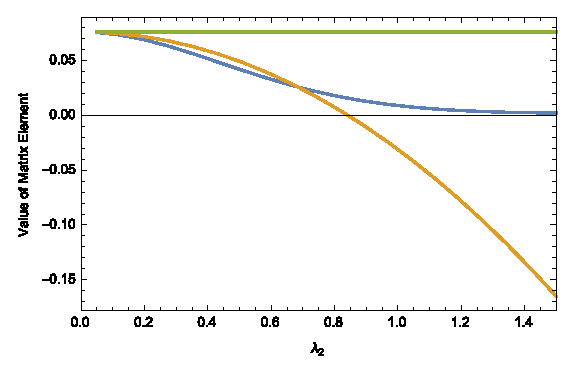
\includegraphics[width=0.6\textwidth]{LocalExpansion/Figures/ToyPotential000000} 
\caption{Matrix elements of $\braket{n'=0,\: l'=0,\: m_l'=0 | V | n=0,\: l=0,\: m_l=0}$ for $b=\lambda_1=1$ as a function of $\lambda_2$. The blue line shows the exact numerically evaluated matrix elements, while the orange line shows the second order Taylor approximation.
\label{fig:gaussToy1}}
\end{figure}

Matrix elements of the potential \eqref{eq:gaussToy} compare qualitatively as expected. First, we see that the exact values and the Taylor approximation converge for $\lambda_2\rightarrow 0$ in \Cref{fig:gaussToy1} but that the error increases as the range parameter $\lambda_2$ becomes non-perturbatively large. \Cref{fig:gaussToy2} demonstrates that the convergence is essentially independent of $\lambda_1$. Higher angular momenta are more difficult to integrate numerically, 

%One interesting observation in the second order approximation is that the second derivative in $\lambda_2$ of the matrix elements is strictly negative for all of the channels tested, although this is not true for the exact results. Does the addition of fourth order terms (the third order terms are zero) introduce contributions which change this situation?

\begin{figure}[htb]
\centering 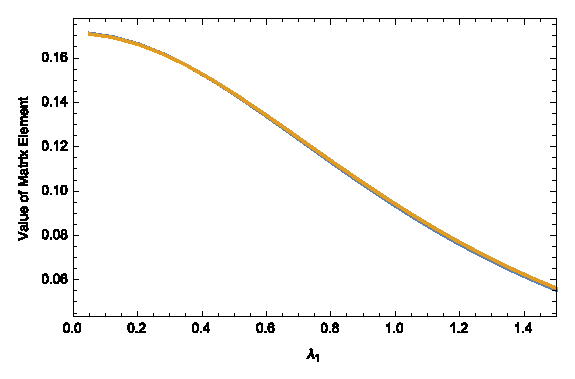
\includegraphics[width=0.6\textwidth]{LocalExpansion/Figures/ToyPotential000000l1} 
\caption{Matrix elements of $\braket{n'=0,\: l'=0,\: m_l'=0 | V | n=0,\: l=0,\: m_l=0}$ for $b=1$, $\lambda_2=0.05$ as a function of $\lambda_1$. The blue line shows the exact numerically evaluated matrix elements, while the orange line shows the second order Taylor approximation.
\label{fig:gaussToy2}}
\end{figure}



\end{section}
%%%%%%%%%%%%%%%%%%%%%%%%%%%%%%%%%%%%%%%%%%%%%%%%
\begin{section}{Comparison of nonlocal and local approximations to the in-medium effective term $V_D$ }

\end{section}


\chapter{\label{chap:SOC}Energy Spectra of Two Interacting Fermions with Spin-Orbit Coupling in a Harmonic Trap}

%\begin{abstract}
%We explore the two-body spectra of spin-$1/2$ fermions in isotropic harmonic traps with external spin-orbit potentials and short range two-body interactions. Using a truncated basis of total angular momentum eigenstates, nonperturbative results are presented for experimentally realistic forms of the spin-orbit coupling: a pure Rashba coupling, Rashba and Dresselhaus couplings in equal parts, and a Weyl-type coupling. The technique is easily adapted to bosonic systems and other forms of spin-orbit coupling.
%\end{abstract}

Cold atomic gases with parity-violating spin-orbit coupling (SOC) have recently been an area of intense interest because of the potential to simulate interesting physical systems with precisely tunable interactions \cite{nature11841}. In condensed-matter and atomic physics, spin-orbit couplings\footnote{In these fields, spin-orbit coupling conventionally refers to operators which couple spin with momentum, as opposed to the more restrictive use in nuclear and atomic physics where there term specifically refers to a parity-conserving $\vec{\ell}\cdot \vec{s}$ interaction.}\ are essential for many exotic systems such as topological insulators \cite{das2013engineering,PhysRevLett.105.255302}, the quantum spin Hall effect \cite{nature12185}, and spintronics \cite{RevModPhys.76.323}. The experimental setup which induces spin-orbit coupling is intimately related to simulation of synthetic gauge fields \cite{RevModPhys.83.1523,hamner2014dicke,Lin:2009zzb,Bermudez:2011db}. Because these couplings are parity violating, they potentially play similar roles within nuclear systems that undergo parity-violating transitions due to the nuclear weak force.  Atomic gases provide an excellent testing ground both to explore universal behavior of these real life systems and to create new types of spin-orbit coupling which are not yet known to exist (or have no solid-state analog) in other materials but are interesting in their own right. Further, these experiments can be performed in an environment with few or no defects and impurities.

Spin-orbit coupling was first realized in a Bose condensate of $^{87}$Rb \cite{nature09887} and extended shortly after to Fermi gases of $^{40}$K \cite{PhysRevLett.109.095301} and $^6$Li \cite{PhysRevLett.109.095302}. These spin-orbit interactions are `synthetic' in the sense that a subset of the hyperfine states stand in as virtual spin states. A particularly interesting consequence of this is the possibility of studying systems with synthetic spin-$1/2$ spin-orbit interactions but bosonic statistics \cite{PhysRevA.68.063612,nature09887}. From another point of view, the couplings are equivalent to applying external electromagnetic forces via synthetic gauge couplings on the physically uncharged particles in the gas \cite{Lin:2011,PhysRevLett.107.255301}. It has also been conjectured that these systems could be used to physically simulate lattice gauge theories \cite{Bermudez:2010da,Mazza:2011kf}.  Spin-orbit couplings in solid-state systems arise in two-dimensional (2D) systems (Rashba and Dresselhaus types, described in Sec.~\ref{sec:Hamiltonian}), but recently an experimental setup has been proposed that can simulate the Weyl-type SOC which is fundamentally three dimensional \cite{PhysRevLett.108.235301}.

Spin-orbit couplings are also of interest from the perspective of few-body physics where they arise in a variety of fields, e.g., the weak nuclear interactions governing proton-proton scattering \cite{Haxton:2013aca,deVries:2014vqa}. Because the spin-orbit coupling is long range, it can significantly modify both the threshold scattering behavior and the spectrum of two-body systems \cite{PhysRevA.86.042707}. For low-energy scattering, Duan \textit{et al.} \cite{PhysRevA.87.052708} showed analytically that parity-violating SOC leads to the the spontaneous emergence of handedness in outgoing states, a finding later confirmed in \cite{PhysRevA.91.022706}. Even in the presence of a repulsive two-body interaction, an arbitrarily weak SOC has been shown to bind dimers \cite{PhysRevB.83.094515}. For three-particle systems, a new type of universality is conjectured to occur for bound trimers with negative scattering length \cite{PhysRevLett.112.013201}. 

Few-atom systems undergoing SOC within trapping potentials have also been explored. For example, the spectrum of particles within a trap with an external SOC of the Weyl type (but no relative interaction) has been theoretically determined \cite{anderson2013}. The Rashba SOC with two-particle systems interacting via short-ranged interactions was investigated perturbatively in \cite{PhysRevA.89.033606}, where it was shown that the leading order corrections due to the SOC and short-range interaction are independent when the scattering length is equal for all channels.  In one dimension, the spectrum for this type of system has been calculated when the SOC consists of equal parts Rashba and Dresselhaus interactions \cite{guan2014energy}. Information learned from trapped systems augments that from scattering experiments while also being relevant to interesting phenomena in trapped many-body systems with SOC such as solitons \cite{DarkSolitons,PhysRevA.87.013614} or novel phase diagrams \cite{PhysRevLett.107.270401}.


In all these calculations, the emergent spectrum is rich and complex, offering new insights into few-body behavior.  Our objective is to provide some additional insight into two-body physics of Fermi gases with spin-orbit interactions in the presence of both three-dimensional trapping potentials and short-ranged two-body interactions, which are necessarily present in dilute cold-atom experiments. Our approach is to numerically diagonalize the Hamiltonian within a suitably truncated basis, and is thus nonperturbative in nature. Eigenstates of the interacting Hamiltonian without SOC are used for the basis. Section~\ref{sec:Hamiltonian} introduces the specific forms of spin-orbit coupling and two-body interactions which we consider. The general method is detailed in Sec.~\ref{sec:Weyl} for the simplest SOC.  In the remaining Secs.~\ref{sec:Rashba}-\ref{sec:R=D} we study the spectra of additional spin-orbit couplings in order of increasing computational complexity.

\section{\label{sec:Hamiltonian}Hamiltonian for Spin-orbit Couplings with Contact Interactions}

In this chapter we simply refer to our systems by their `spin' degrees of freedom and use the standard notation for spin quantum numbers. We consider three different types of spin-orbit coupling. The form of spin-orbit coupling realized in experiments is a linear combination of the Rashba \cite{0022-3719-17-33-015} and linear Dresselhaus \cite{PhysRev.100.580} types,
\begin{align}
V_{R}&\equiv\alpha_R (\sigma_x k_y-\sigma_y k_x) \label{eq:Rashba},\\
V_{D}&\equiv\alpha_D (\sigma_x k_y+\sigma_y k_x) \label{eq:Dresselhaus},
\end{align} 
which were originally recognized in two-dimensional solid-state systems. In a 2D system, these form a complete basis for spin-orbit couplings linear in momentum. Note that some references use the alternate definitions $V_R\propto  (\sigma_x k_x+\sigma_y k_y) $ and $V_D\propto  (\sigma_x k_x-\sigma_y k_y) $ which are equivalent up to a pseudospin rotation.  For solids, these parity-violating interactions are allowed only in the absence of inversion symmetries. Rashba-type SOC typically arises in the presence of applied electric fields or in 2D subspaces such as the surfaces of materials where the boundary breaks the symmetry. Dresselhaus couplings were first studied in the context of bulk inversion asymmetry, when the internal structure leads to gradients in the microscopic electric field. 

To date, experiments have produced only SOC potentials in which the Rashba and Dresselhaus terms appear with equal strength (also known as the ``persistent spin-helix symmetry point'' \cite{PhysRevLett.97.236601}), 
\begin{equation}
\label{eq:R=D}
V_{R=D}\equiv\alpha_{R=D}\sigma_x k_y.
\end{equation} 
After a pseudospin rotation, this potential can be seen as a unidirectional coupling of the pseudospin and momentum along a single axis. A proposal for tuning the ratio $\alpha_R/\alpha_D$ has been given in \cite{PhysRevA.84.025602}.  An experimental setup which gives the simple three-dimensional Weyl coupling,
\begin{equation}\label{eq:Weyl}
V_{W}\equiv\alpha_W \vec{k}\cdot\vec{\sigma},
\end{equation}
has also been proposed in \cite{PhysRevLett.108.235301} and \cite{PhysRevLett.111.125301}. 

In the following sections we calculate the spectra of two particles with a short-range two-body interaction, an isotropic harmonic trapping potential and spin-orbit coupling. The single particle Hamiltonian is 
\begin{equation}\label{eq:shortRangeInteraction}
H_1=\frac{\hbar^2 k^2}{2m}+\frac{1}{2}m\omega^2 r^2 + V_{\text{SO}}.
\end{equation}
For the spin-orbit term $V_{\text{SO}}$, we consider equal Rashba and Dresselhaus~\eqref{eq:R=D}, pure Rashba~\eqref{eq:Rashba}, and Weyl~\eqref{eq:Weyl} spin-orbit couplings  because these are generally considered to be experimentally feasible.

We assume that the range of interaction between particles is small compared to the size of the oscillator well.  The relative interaction between the particles can then be approximated as a regulated $s$-wave contact interaction, which in momentum space (as a function of relative momentum) is given by
\begin{equation}
\frac{4\pi \hbar^2}{m}a(\Lambda)\ .
\end{equation}
Here the argument $\Lambda$ refers to some cutoff scale and $a(\Lambda)$ is some function of the cutoff and physical scattering length $a_{\text{phys}}$.  The exact form of this function depends on the type of regulator used and is not relevant for this work; the only constraint is that $a(\Lambda)$ reproduce the physical scattering length given by the scattering $T$ matrix at threshold, $T(E=0)=4\pi\hbar^2 a_{\text{phys}}/m$ \cite{taylor2000}. In the limit $\Lambda\rightarrow \infty$ the spectrum of two particles in an oscillator well (without external spin-orbit interaction) was solved by Busch \textit{et al.} \cite{Busch} using the method of pseudopotentials.  In Ref.  \cite{Luu:2006xv} the solution for general $\Lambda$ was given using a Gaussian regulator, which in the limit $\Lambda\rightarrow\infty$ recovered the Busch \textit{et al.} solution.  For our work below we use the eigenstates and eigenvalues of this two-particle system given in Ref. \cite{Busch}.

\section{\label{sec:Weyl}Weyl Coupling}
We tackle the Weyl form first because of its mathematical and numerical simplicity. In the absence of the two-body interaction, this problem was treated in Ref. \cite{anderson2013}. Our approach is to determine the matrix elements of the SOC in an appropriate basis. The eigenvalue is then solved numerically at the desired precision by choosing an appropriately large truncated basis of harmonic oscillator (HO) eigenstates.

As usual, the two-body problem is best approached in the dimensionless Jacobi coordinates
\begin{equation}
R=\frac{r_1+r_2}{\sqrt{2}b}, \qquad r=\frac{r_1-r_2}{\sqrt{2}b}
\end{equation}
and the corresponding conjugate momenta $q,Q$ representing the relative and total momenta. For an isotropic harmonic oscillator, distances can be expressed in terms of the ground-state length scale $b=\sqrt{\hbar/m\omega}$ and energies will be similarly measured in units of $E_0=\hbar\omega$. We also define the spin operators
\begin{equation}
\vec{\sigma}\equiv\vec{\sigma}_1-\vec{\sigma}_2, \qquad \vec{\Sigma}\equiv\vec{\sigma}_1+\vec{\sigma}_2.
\end{equation}

With these definitions, the two-body Hamiltonian can be nondimensionalized and separated into relative and center-of-mass (c.m.) parts,
\begin{equation}\label{eq:WeylHamiltonian}
\frac{1}{\hbar\omega}H=\left(h_{0,\text{rel}}+\frac{\tilde{\alpha}_W}{\sqrt{2}} \vec{q}\cdot\vec{\sigma} + \sqrt{2}\pi \tilde{a}(\Lambda) \delta^{(3)}(r)\right)+\left(h_{0,\text{c.m.}}+\frac{\tilde{\alpha}_W}{\sqrt{2}} \vec{Q}\cdot\vec{\Sigma} \right),
\end{equation}
where $h_{0,\text{rel}}=r^2/2$ and $h_{0,\text{c.m.}}=R^2/2$. Notably, the spin-orbit coupling appears in both terms.  The tilde over the coupling constants indicates that they are dimensionless, related to the original coupling constants by e.g., $\tilde{\alpha}_W=\alpha_W/(\hbar\omega b)$. Similarly the scattering length is made dimensionless by dividing out the oscillator length, $\tilde{a}=a/b$. Throughout the remainder of this chapter we will refer to dimensionless eigenvalues of $H/\hbar\omega$ as the energies of the system.

%We point out that the relative-coordinate spin-orbit term in Eq.~\eqref{eq:WeylHamiltonian} is exactly of the form that appears in weak-interaction parity-violating proton-proton scattering \cite{Haxton:2013aca,deVries:2014vqa}.  Aside from Coulomb contributions, the $^1S_0$ channel of proton-proton scattering has a scattering length that is an order of magnitude larger than its effective range.  The parity-conserving part of the nuclear potential could therefore be represented by the contact interaction in Eq.~\eqref{eq:WeylHamiltonian}.  The CM spin-orbit term (i.e. the last term in Eq.~\eqref{eq:WeylHamiltonian}) spoils this analogy. However, we will show later that the effect of this term on the ground state is negligible. 

\begin{figure}
\centering
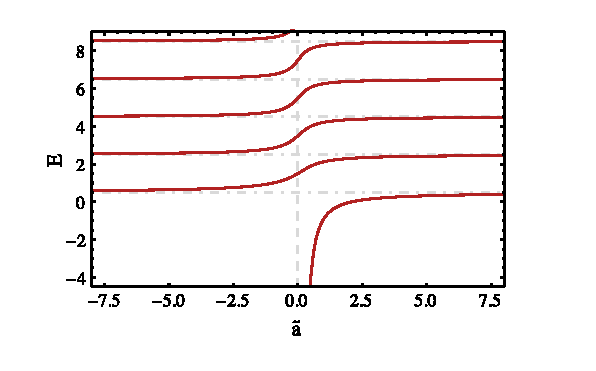
\includegraphics[scale=1.2]{SOC/Figures/BuschSpectrum}
\caption[Spectrum of the two-body contact interaction Hamiltonian as a function of $\tilde a$]{\label{fig:BuschSpectrum} Spectrum of the two-body contact interaction Hamiltonian as a function of $\tilde a$. The horizontal lines indicate the dimensionless energy eigenvalues in the unitary limit $|\tilde{a}|\rightarrow\infty$.} 
\end{figure}

Eigenstates of two particles with a short-range interaction in a harmonic oscillator trapping potential form a convenient basis for these calculations. These basis functions were first derived in \cite{Busch} for the isotropic case considered here, and the more general case of an anisotropic trap has been explored in \cite{PhysRevA.74.022712}. The dependence of the energy spectrum on the scattering length $a$ is shown in Fig.~\ref{fig:BuschSpectrum} for reference. Qualitatively, the effect of the short-range interaction is to shift the harmonic oscillator energies by $\pm \hbar\omega$ as the scattering length goes to $\pm \infty$. For positive scattering length, there is also an additional negative-energy dimer state.

We choose the particular coupling scheme of angular momentum eigenstates,
\begin{equation}\label{eq:basisStates}
\ket{n(ls)j;NL;(jL)J},
\end{equation}
which simplify the matrix elements for the relative-coordinate operators. Here $n$ and $l$ refer to the principal and orbital angular-momentum quantum numbers of the two-particle system in the relative coordinates. $N$ and $L$ refer to the analogous numbers in the center-of-mass frame. The total spin of the two spin-$1/2$ particles is denoted by $s = s_1 + s_2$ and may be either 0 or 1. First $s$ and $l$ to make angular momentum $j$, which is then recoupled with the c.m. angular momentum $L$ to make the state's total angular momentum $J$. Because all terms in the Hamiltonian~\eqref{eq:WeylHamiltonian} are scalars, the interaction is independent of $J_z$ and so we omit this quantum number for clarity. Due to Pauli exclusion, $l + s$ must be even to enforce antisymmetry under exchange of the particles.

For $l\neq0$ the states~\eqref{eq:basisStates} are identical to the well known harmonic oscillator, with $n$ and $l$ ($N$ and $L$) indicating the relative (center-of-mass) HO quantum numbers. We use the convention that $n,N=0,1,2,\dots$, and therefore $E=2n+l+2N+L+3$. The short range interaction~\eqref{eq:shortRangeInteraction} modifies the $l=0$ states and their spectrum. The principal relative quantum number $n$ for these states is obtained by solving the transcendental equation
\begin{equation}\label{eq:eigenvalueEqn}
\sqrt{2}\frac{\Gamma(-n)}{\Gamma(-n-1/2)}=\frac{1}{\tilde{a}}
\end{equation}
and is no longer integer valued. For the relative-coordinate part of the $l=0$ wave function,
\begin{align}
\phi(r)&=\frac{1}{2\pi^{3/2}}A(n)\Gamma(-n)U(-n,3/2,r^2)e^{-r^2/2}, \label{eq:BuschWF}\\
A(n)&=\left(\frac{\Gamma(-n)[\psi_0(-n)-\psi_0(-n-1/2)]}{8 \pi^2 \Gamma(-n-1/2)}\right)^{-1/2},
\end{align}
where $U(a,b,x)$ is Kummer's confluent hypergeometric function and $\psi_0(x)=\Gamma'(x)/\Gamma(x)$ is the digamma function. A derivation of the normalization factor $A(n)$ is given in the Appendix.

Standard angular momentum algebra can be used to determine the matrix elements of the two spin-orbit coupling terms; we follow the conventions of \cite{Edmonds}. For Weyl SOC of two spin-$1/2$ fermions, the matrix elements of the coupling in the relative momentum are
\begin{equation}\label{eq:WeylRel}\begin{split}
\bra{n'(l's')j';N'L';(j'L')J'}\vec{q}&\cdot\vec{\sigma} \ket{n(ls)j;NL;(jL)J}  \\
=&\delta_{N,N'}\delta_{L,L'}\delta_{j,j'}\delta_{J,J'}(-1)^{l+s'+j}\frac{3}{\sqrt{2}}\sixj{j}{s'}{l'}{1}{l}{s} (s'-s)\braket{n'l' || q || n l}.
\end{split}
\end{equation}
To preserve anti-symmetry of the two-particle system, the relative momentum term in the Weyl SOC must couple states with relative angular momentum $l$ to $l\pm 1$, leaving $l+s$ even but changing the parity.

For basis states with both $l,l'\neq0$, reduced matrix elements of the momentum operator are calculated between pure harmonic oscillator states,
% Could do away with some constants in favor of the 3-j coefficient
\begin{align}
\braket{n'l' || q || n l}=&(-1)^{l'}(-1)^{\frac{l+l'+1}{2}}\sqrt{\frac{2(2l+1)(2l'+1)}{(l+l'+1)}}\braket{n'l'0| (-i \nabla_0) | n l 0} \\
\begin{split} =& i(-1)^{l}\sqrt{\frac{l+l'+1}{2}}\sqrt{n!n'!\Gamma(n+l+3/2)\Gamma(n'+l'+3/2)} \\ 
&\times\sum_{m,m'=0}^{n,n'} \left\{
     \begin{array}{lr}
       \frac{(-1)^{m+m'}\left[2m\Gamma\left(m+m'+1+\frac{l+l'}{2}\right)-\Gamma\left(m+m'+1+\frac{l+l'}{2}\right)\right]}{m!m'!(n-m)!(n'-m')!\Gamma(m+l+3/2)\Gamma(m'+l'+3/2)} & \text{if}\: l'=l-1 \\
        \frac{(-1)^{m+m'+1}\left[(2m+2l+1)\Gamma\left(m+m'+1+\frac{l+l'}{2}\right)-\Gamma\left(m+m'+1+\frac{l+l'}{2}\right)\right]}{m!m'!(n-m)!(n'-m')!\Gamma(m+l+3/2)\Gamma(m'+l'+3/2)} & \text{if}\: l'=l+1 \\
       0 & \text{otherwise}
     \end{array}
   \right.
   \end{split}
\end{align}
If $l=1$ and $l'=0$ or vice versa, reduced matrix elements between one modified wave function of the form~\eqref{eq:BuschWF} and one pure harmonic oscillator state are needed. These are given by
\begin{align}
\braket{n l=0 || q || n' l'=1}=-i A(n) \sqrt{\frac{\Gamma(n'+5/2)}{2\pi^3 n'!}}\frac{2n-2n'-1}{2(n'-n)(1+n'-n)}
\end{align}
and its Hermitian conjugate.

Our choice of basis makes the relative matrix elements~\eqref{eq:WeylRel} simple at the cost of complicating the center-of-mass term. We take the approach of expanding the states~\eqref{eq:basisStates} in the alternate coupling scheme,
\begin{equation}\label{eq:basisStates2}
\ket{n(ls)j;NL;(jL)J}=(-1)^{l+s+L+J}\sqrt{2j+1}\sum_{\mathcal{J}}\sqrt{2\mathcal{J}+1}\sixj{l}{s}{j}{L}{J}{\mathcal{J}}\ket{nl;N(Ls)\mathcal{J};(l\mathcal{J})J}.
\end{equation}
Using this notation, the matrix elements can be written
\begin{equation}\begin{split}
\bra{n'(l's')j';N'L';(j'L')J'}&\vec{Q}\cdot\vec{\Sigma} \ket{n(ls)j;NL;(jL)J} = \delta_{n,n'}\delta_{l,l'}\delta_{J,J'}\delta_{s,1}\delta_{s1,1}   6 (-1)^{L} \\
&\hspace{-2cm}\times\braket{N'L'|| \vec{Q} || NL} \sum_{\mathcal{J}}(-1)^\mathcal{J} (2\mathcal{J}+1)\sixj{l}{1}{j'}{L'}{J}{\mathcal{J}}\sixj{l}{1}{j}{L}{J}{\mathcal{J}}\sixj{\mathcal{J}}{1}{L'}{1}{L}{1}.
\end{split}
\end{equation}
Again, the reduced matrix element of the center-of-mass momentum changes the parity by connecting states with $\Delta L=\pm1$. Matrix elements are nonzero only for $\Delta s=0$ because the antisymmetry of the spatial wave function depends only on $l$, which does not change. We also note that the c.m. term does not affect states with singlet spin wave functions ($s=0$).


\begin{figure}
\centering
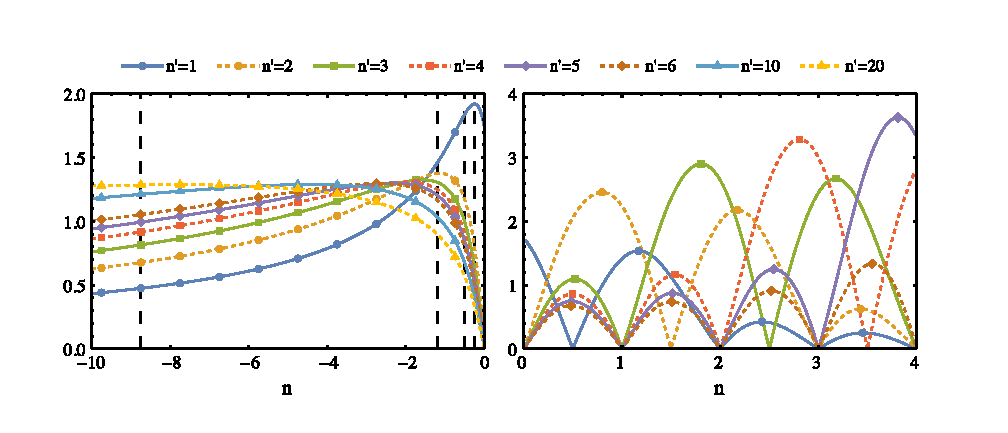
\includegraphics{SOC/Figures/MatrixElts}
\caption[Coupling of ground state to $l=1$ states for the Weyl spin-orbit Hamiltonian]{\label{fig:matrixElts}Absolute value of the matrix elements $|\bra{n'(11)0;00;(00)0}\vec{\sigma}\cdot\vec{q}\ket{n(00)0;00;(00)0}|$ between the ground state and $l=1$ excited states. The horizontal axis is the principal quantum number of the ground state obtained by solving~\eqref{eq:eigenvalueEqn}. From left to right, the vertical lines on the negative axis indicate the values obtained for $\tilde{a}=1/4$, $\tilde{a}=1$, $\tilde{a}=\pm\infty$, and $\tilde{a}=-1$, respectively.} 
\end{figure}

Using these matrix elements, we calculated the spectrum of the two interacting particles with Weyl spin-orbit coupling. Our calculations are performed by numerically diagonalizing in a truncated basis of the harmonic oscillator states~\eqref{eq:basisStates}, where a cutoff $2N+L+\nobreak 2n+\nobreak l+ \nobreak3\leq\nobreak E_{\text{max}}$ is set high enough that the eigenvalues of the matrix have converged to the desired accuracy.  

\begin{figure}
\centering
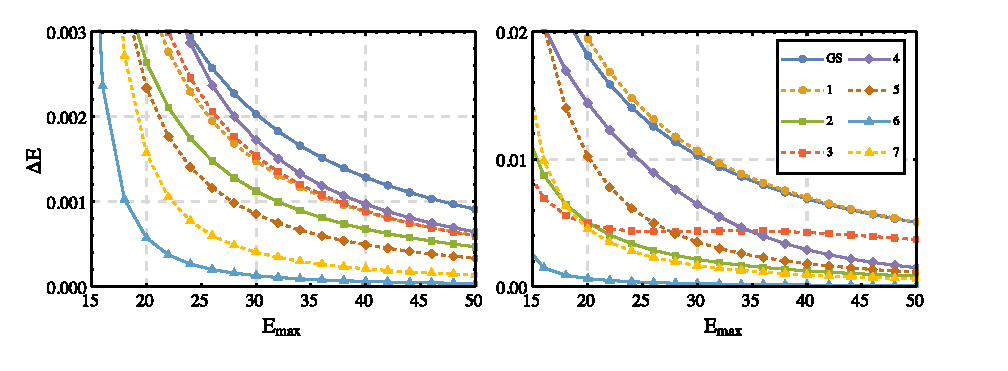
\includegraphics{SOC/Figures/WeylConvergence}
\caption[Convergence of the energy eigenvalues for the Weyl spin-orbit coupling]{\label{fig:WeylConvergence}  A convergence plot giving the change in energy eigenvalue, $\Delta E$, for the lowest eight energy levels when a shell is added as a function of $E_{\text{max}}$.  The left figure shows convergence for $\tilde{a}=-1$ and $\tilde{\alpha}_W=0.5$. In the right panel  we show $\tilde{a}=1$ and $\tilde{\alpha}_W=0.5$, demonstrating that convergence of the states with large negative $n$ is poor.} 
\end{figure}

This approach converges well only when the ground-state energy is not too low. In particular, for $a$ positive but very small the principal quantum number of the ground state is increasing from negative infinity as seen in Fig.~\ref{fig:BuschSpectrum}. From Fig.~\ref{fig:matrixElts}, we can see that as $n$ becomes more negative, the principal quantum number of the dominant matrix element is also increasing. Because convergence of any energy level requires a cutoff much larger than the energy of the most strongly coupled states, a sufficiently high $E_{\text{max}}$ to ensure an accurate ground-state energy becomes infeasible for small positive $a$. For excited states, $n$ is always positive and matrix elements with similar $n$ always dominate. The strength of the matrix elements follows a similar qualitative behavior for the spin-orbit couplings treated in the following sections where the same issues recur. 

\begin{figure}
\centering
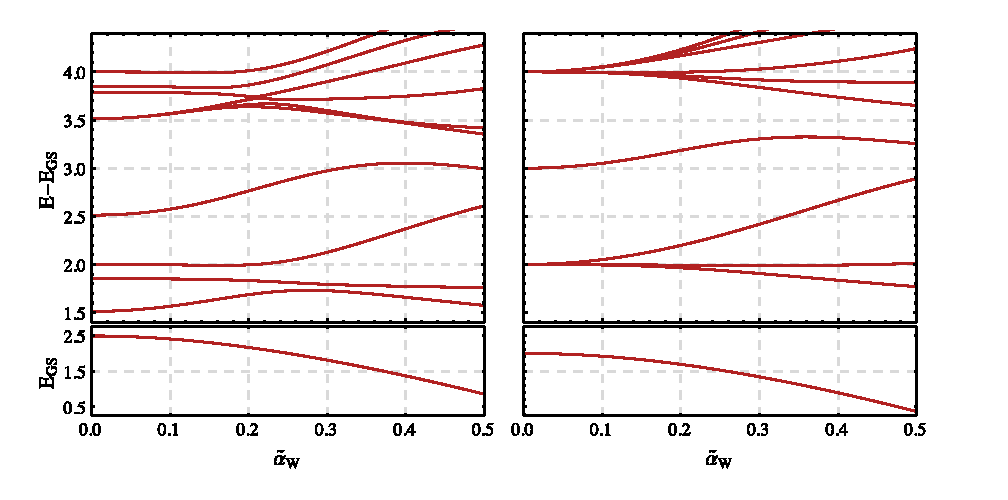
\includegraphics{SOC/Figures/WeylSpectrum}
\caption[Spectrum of states with $J=0$ for Weyl spin-orbit coupling]{\label{fig:WeylSpectrum}  Spectrum of states with total angular momentum $J=0$ for the dimensionless Hamiltonian~\eqref{eq:WeylHamiltonian}. The bottom left figure shows the ground-state energy for $\tilde{a}=-1$ as a function of $\tilde{\alpha}_W$; above are the first few excitation energies. The right figure shows the results in the unitary limit of the two-body interaction, $|\tilde{a}|\rightarrow\infty$. The spectrum is symmetric about $\tilde{\alpha}_W=0$.} 
\end{figure}

As a result, convergence of the ground state is actually slower than that for nearby excited states. Furthermore, our approach gives the fastest convergence when $a$ is not small and positive. We compare the rate of convergence of the $\tilde{a}=-1$ and $\tilde{a}=1$ spectra in Fig.~\ref{fig:WeylConvergence} to demonstrate the dependence of convergence on the matrix truncation. The actual energy spectrum is shown in Fig.~\ref{fig:WeylSpectrum}. 

\begin{figure}
\centering
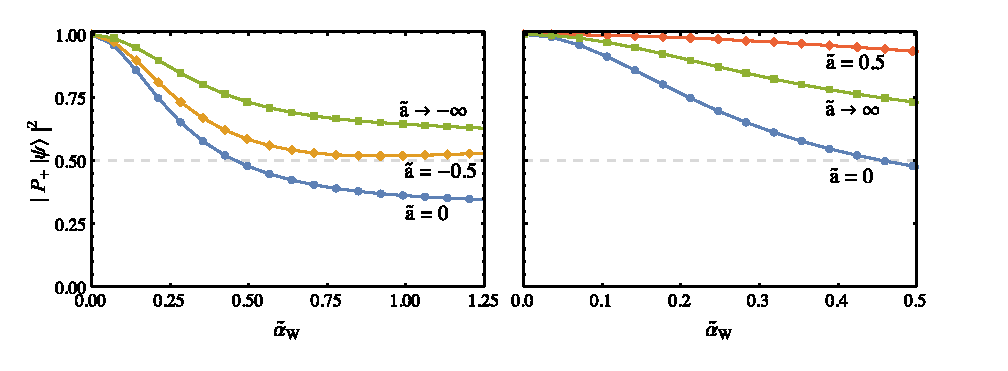
\includegraphics{SOC/Figures/Projections}
\caption[Parity projection of the Weyl spin-orbit coupling ground state]{\label{fig:Projections} For different values of the two-body coupling strength $\tilde{a}$, we show the magnitude of the ground state projected onto even parity basis states as a function of the SOC strength. This is given by $\big|  P_+\ket{\psi_{\text{GS}}}\big|^2=\big| (1- P_-)\ket{\psi_{\text{GS}}}\big|^2$, where $P_+$ ($P_-$) is the projection operator onto the positive\nobreak- (negative\nobreak-) parity basis states. The left figure shows negative $\tilde{a}$, while the right shows positive $\tilde{a}$. Note that the limits $\tilde{a}\rightarrow\pm\infty$ are physically identical.}
\end{figure}

One consequence of parity violation in this system is that the eigenstates are mixtures of the even- and odd-parity basis states described by Eq.~\eqref{eq:basisStates}. In Fig.~\ref{fig:Projections} we visualize how these subspaces are mixed in the ground state as the SOC strength increases. For the noninteracting system, $\tilde{a}=0$, more than half of the ground state projects onto negative-parity states even at fairly small values of $\tilde{\alpha}_W$. However, we see that the short-range interaction reduces this effect. With negative $\tilde{a}$, the mixing of the negative-parity states is suppressed as the strength of the two-body interaction increases. When $\tilde{a}$ is positive the effect is more striking. Mixing with negative-parity states is most strongly suppressed for small positive values of $\tilde{a}$, while the projection onto these states increases for larger positive values. The admixture is qualitatively the same when considering other forms of SOC as described in the following sections.

\section{\label{sec:Rashba}The Pure Rashba Coupling}

In order to find the matrix elements of the pure Rashba coupling given in~\eqref{eq:Rashba}, we first note that it can be written as a spherical tensor
\begin{equation}
V_{R}=i\sqrt{2}\:\alpha_R \left[ k \otimes \sigma \right]_{10}.
\end{equation}
We therefore have the two-body Hamiltonian
\begin{equation}\label{eq:RashbaHamiltonian}
\frac{1}{\hbar\omega}H=\left(h_{0,\text{rel}}+i \tilde{\alpha}_R  \left[ \vec{q} \otimes \vec{\sigma} \right]_{10} + \sqrt{2}\pi \tilde{a}(\Lambda) \delta^{(3)}(r)\right)+\left(h_{0,\text{c.m.}}+i \tilde{\alpha}_R [ \vec{Q}\otimes \vec{\Sigma} ]_{10} \right).
\end{equation}

Because the spin-orbit coupling is now a $k=1$ tensor rather than a scalar operator, the total angular momentum $J$ is no longer conserved. Additionally, the matrix elements now depend on the quantum number $J_z$ (which is conserved). For the relative-coordinate part of the SOC, some algebra gives
\begin{equation}\begin{split}
&\bra{n'(l's')j';N'L';(j'L')J'J'_z}  [ \vec{q} \otimes \vec{\sigma} ]_{10}  \ket{n(ls)j;NL;(jL)JJ_z} = \\
&\hspace{1.5cm} 6 i (-1)^{J+J'-J'_z+j'+L+1}\delta_{N,N'}\delta_{L,L'}\delta_{J_z,J'_z} \sqrt{(2J+1)(2J'+1)(2j+1)(2j'+1)} \\
 &\hspace{2.7cm} \times \threej{J'}{1}{J}{-J_z}{0}{J_z} \sixj{j'}{J'}{L}{J}{j}{1}
 \renewcommand{\arraystretch}{0.9}
 \ninej{\hphantom{l}l'\hphantom{l}}{\hphantom{l}l\hphantom{l}}{\hphantom{l}1\hphantom{l}}{s'}{s}{1}{j'}{j}{1} (s'-s) \braket{n'l' || q || n l}.
\end{split}
\end{equation}
For the center-of-mass part of the Hamiltonian we again expand the basis states in the alternate coupling scheme~\eqref{eq:basisStates2} to obtain the matrix elements
\begin{equation}\begin{split}
&\bra{n'(l's')j';N'L';(j'L')J'J'_z} [ \vec{Q} \otimes \vec{\Sigma} ]_{10}  \ket{n(ls)j;NL;(jL)JJ_z} = \delta_{n,n'}\delta_{l,l'}\delta_{J_z,J'_z}\delta_{s,1}\delta_{s',1} \\
 &\quad\times 6 i \sqrt{2}(-1)^{J+J'-J'_z+l} \sqrt{(2J+1)(2J'+1)(2j+1)(2j'+1)} \threej{J'}{1}{J}{-J_z}{0}{J_z}  \braket{N' L' || Q || N L} \\ 
 &\quad\times\sum_{\mathcal{J},\mathcal{J}'} (-1)^\mathcal{J}(2\mathcal{J}+1)(2\mathcal{J}'+1)\sixj{l}{1}{j'}{L'}{J'}{\mathcal{J}'}\sixj{l}{1}{j}{L}{J}{\mathcal{J}}\sixj{\mathcal{J}'}{J'}{l}{J}{\mathcal{J}}{1}
 \renewcommand{\arraystretch}{0.9}
 \ninej{\hphantom{l}L'\hphantom{l}}{\hphantom{l}L\hphantom{l}}{\hphantom{l}1\hphantom{l}}{1}{1}{1}{\mathcal{J}'}{\mathcal{J}}{1} .
\end{split}
\end{equation}

\begin{figure}
\centering
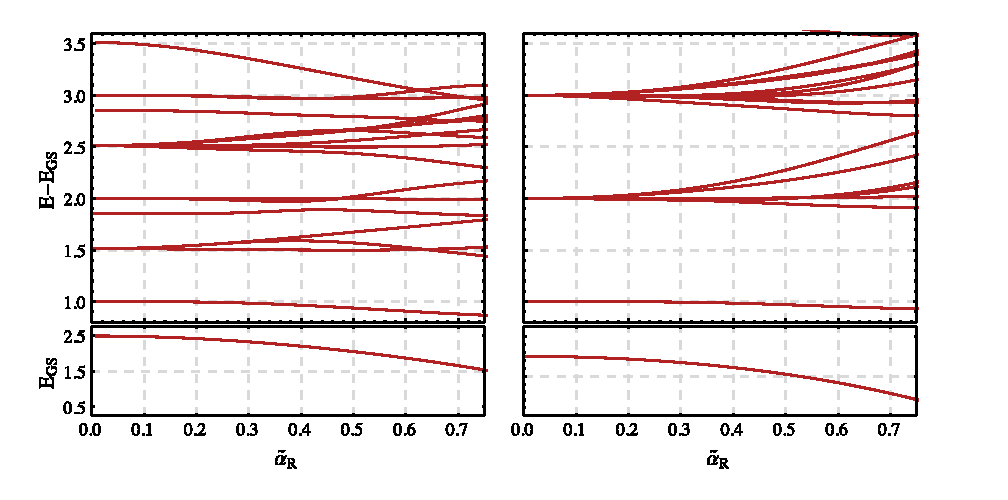
\includegraphics{SOC/Figures/RashbaSpectrum}
\caption[Spectrum of the Rashba spin-orbit coupling for $J_z=0$]{\label{fig:RashbaSpectrum}  Spectrum of states with total angular momentum quantum number $J_z=0$ for the Hamiltonian~\eqref{eq:RashbaHamiltonian}. The left figure shows the energies with negative scattering length $\tilde{a}=-1$. The right figure shows the results in the unitary limit $|\tilde{a}|\rightarrow\infty$. The spectrum is symmetric about $\tilde{\alpha}_R=0$.} 
\end{figure}


Our results for the Rashba SOC are shown in Fig.~\ref{fig:RashbaSpectrum}. Because the Rashba spin-orbit coupling is a vector operator, states of all possible $J$ must be included in any calculation and the size of the basis scales much more quickly with $E_{\text{max}}$. These spectra were computed with an $E_{\text{max}}$ of $24\hbar\omega$, for which there are approximately $36\,000$ basis states. All displayed eigenvalues of the Hamiltonian shift by less than $10^{-2}\hbar\omega$ if an additional shell of states is included.

\begin{figure}
\centering
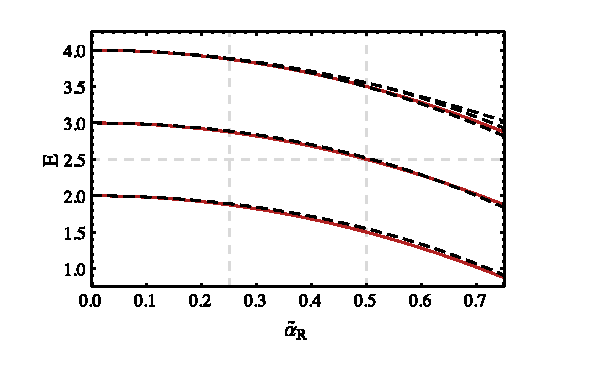
\includegraphics[scale=1.2]{SOC/Figures/PerturbativeComparison}
\caption[Comparison of the Rashba spectrum with perturbative predictions]{\label{fig:ComparisonSpectrum}Comparison of selected spectral lines (dashed black) with the perturbative predictions from \cite{PhysRevA.89.033606} (solid red) when $\tilde{a}=\infty$. }
\end{figure}

\begin{figure}
\centering
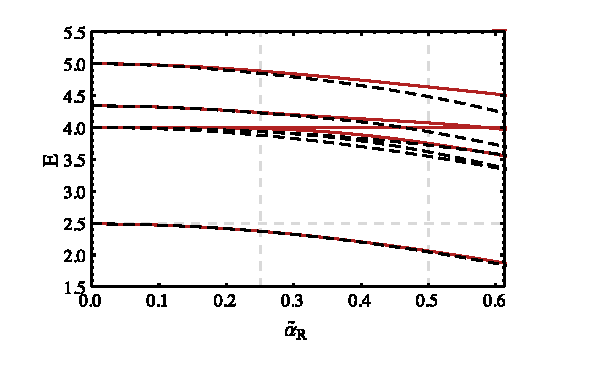
\includegraphics[scale=1.2]{SOC/Figures/ComparisonNoCM}
\caption[Effect of neglecting center of mass excitations for Rashba spin-orbit coupling]{\label{fig:ComparisonSpectrum2}  A comparison of the energy levels with (dashed black) and without (solid red) the inclusion of excitations in the c.m. coordinate for $\tilde{a}=-1$. The approximation of ignoring c.m. excitations provides very accurate results for the ground state, but not for excited states.} 
\end{figure}


This interaction was also studied perturbatively for small $\alpha_R$ in \cite{PhysRevA.89.033606}, including the possibility of a spin-dependent two-body interaction, under the assumption that center-of-mass excitations are unimportant. For the specific case of identical fermions with spin-independent scattering length considered here, they found that the first correction to the energies occurs at order $\alpha_R^2$ and is independent of the scattering length $a$. We compare their perturbative predictions, which are derived from the non-degenerate theory, with our numerical results in Fig.~\ref{fig:ComparisonSpectrum}. 

By setting all matrix elements with $N,L>0$ in the bra or ket to zero, we also explored the approximation of ignoring center-of-mass excitations. Fig.~\ref{fig:ComparisonSpectrum2} shows that this is very accurate for the ground state, but less accurate for excited states. Suppression of the c.m. coordinate has a similar effect for the SOCs considered in Secs.~\ref{sec:Weyl} and~\ref{sec:R=D}. We also note that in the case of small positive $a$, the landscape of low-lying excited states is dominated by center-of-mass excitations. When $a\rightarrow0^+$ in the absence of spin-orbit coupling, there are an infinite number of states with nonzero c.m. quantum numbers whose energies lie between the ground state and the first relative-coordinate excitation.


\section{\label{sec:R=D}Equal-Weight Rashba-Dresselhaus Spin-Orbit Coupling}

Experiments have thus far realized only the effective Hamiltonian with equal strength Rashba and Dresselhaus couplings in the form~\eqref{eq:R=D}. Energy levels of the two-body system in the one-dimensional equivalent of this Hamiltonian with the additional magnetic field couplings present in experimental realizations have been calculated in \cite{guan2014energy}. Here we treat the problem in three dimensions.

This is also the most computationally difficult of the three cases. When decomposed into spherical tensors, the interaction~\eqref{eq:Dresselhaus} becomes
\begin{equation}
V_D=i\,\alpha_D \left( \left[ k \otimes \sigma \right]_{2,-2}- \left[ k \otimes \sigma \right]_{2,2}\right),
\end{equation}
and the two-particle Hamiltonian in the presence of equal strength Rashba and Dresselhaus SOC is given by~\eqref{eq:RashbaHamiltonian} with $\alpha_R\rightarrow \alpha_{R=D}$ plus the additional spin-orbit terms
\begin{equation}\label{eq:DresselhausHamiltonian}
\Delta H= \frac{i \tilde{\alpha}_{R=D}}{\sqrt{2}}\left(  \left[ \vec{q} \otimes \vec{\sigma} \right]_{2,-2} -  \left[ \vec{q} \otimes \vec{\sigma} \right]_{2,2} +[ \vec{Q} \otimes \vec{\Sigma} ]_{2,-2} -  [ \vec{Q} \otimes \vec{\Sigma} ]_{2,2} \right).
\end{equation} 
Yet again the number of basis states with nonzero matrix elements has increased; no angular momentum quantum numbers are conserved. The only remaining selection rule will be that the interaction does not change the total magnetic quantum number $J_z$ between even and odd. 

Using the same approach as in the previous sections, the matrix elements of the relative Dresselhaus term are
\begin{equation}\begin{split}
&\bra{n'(l's')j';N'L';(j'L')J'J'_z} \frac{i \tilde{\alpha}_{R=D}}{\sqrt{2}}\left(  \left[ \vec{q} \otimes \vec{\sigma} \right]_{2,-2} -  \left[ \vec{q} \otimes \vec{\sigma} \right]_{2,2} \right)  \ket{n(ls)j;NL;(jL)JJ_z}  \\
 &\quad\hphantom{\times}= i \sqrt{30}(-1)^{J+J'-J'_z+j'+L}\delta_{N,N'}\delta_{L,L'} \sqrt{(2J+1)(2J'+1)(2j+1)(2j'+1)}  \braket{n'l' || q || n l}\\
 &\hspace{1cm}\quad \times(s'-s) \left[\threej{J'}{2}{J}{-J'_z}{-2}{J_z}-\threej{J'}{2}{J}{-J'_z}{2}{J_z}\right] \sixj{j'}{J'}{L}{J}{j}{2}
 \renewcommand{\arraystretch}{0.9} \ninej{\hphantom{l}l'\hphantom{l}}{\hphantom{l}l\hphantom{l}}{\hphantom{l}1\hphantom{l}}{s'}{s}{1}{j'}{j}{2},
\end{split}
\end{equation}
while the center-of-mass part is 

\begin{equation}\begin{split}
&\bra{n'(l's')j';N'L';(j'L')J'J'_z}  \frac{i \tilde{\alpha}_{R=D}}{\sqrt{2}}\left(  \left[ \vec{Q} \otimes \vec{\Sigma} \right]_{2,-2} -  \left[ \vec{Q} \otimes \vec{\Sigma} \right]_{2,2} \right)  \ket{n(ls)j;NL;(jL)JJ_z}   \\
&\quad=2 i \sqrt{15}(-1)^{J+J'-J'_z+l+1}\delta_{n,n'}\delta_{l,l'}\delta_{s,1}\delta_{s',1}  \\
 &\quad\hphantom{=}\times \sqrt{(2J+1)(2J'+1)(2j+1)(2j'+1)} \left[\threej{J'}{2}{J}{-J'_z}{-2}{J_z}-\threej{J'}{2}{J}{-J'_z}{2}{J_z}\right] \braket{N' L' || Q || N L} \\ 
 &\quad\hphantom{=}\times\sum_{\mathcal{J},\mathcal{J}'} (-1)^\mathcal{J}(2\mathcal{J}+1)(2\mathcal{J}'+1)\sixj{l}{1}{j'}{L'}{J'}{\mathcal{J}'}\sixj{l}{1}{j}{L}{J}{\mathcal{J}}\sixj{\mathcal{J}'}{J'}{l}{J}{\mathcal{J}}{2}
 \renewcommand{\arraystretch}{0.9}
 \ninej{\hphantom{l}L'\hphantom{l}}{\hphantom{l}L\hphantom{l}}{\hphantom{l}1\hphantom{l}}{1}{1}{1}{\mathcal{J}'}{\mathcal{J}}{2} .
\end{split}
\end{equation}

The richly structured excitation spectrum of low-lying states is shown in Fig.~\ref{fig:R=DExcitationSpectrum} for a cutoff of $E_{\text{max}}=17$. All displayed energies shift by less than .$02\hbar\omega$ when the final shell is added, giving a slightly faster convergence than in the pure Rashba case.

\begin{figure}
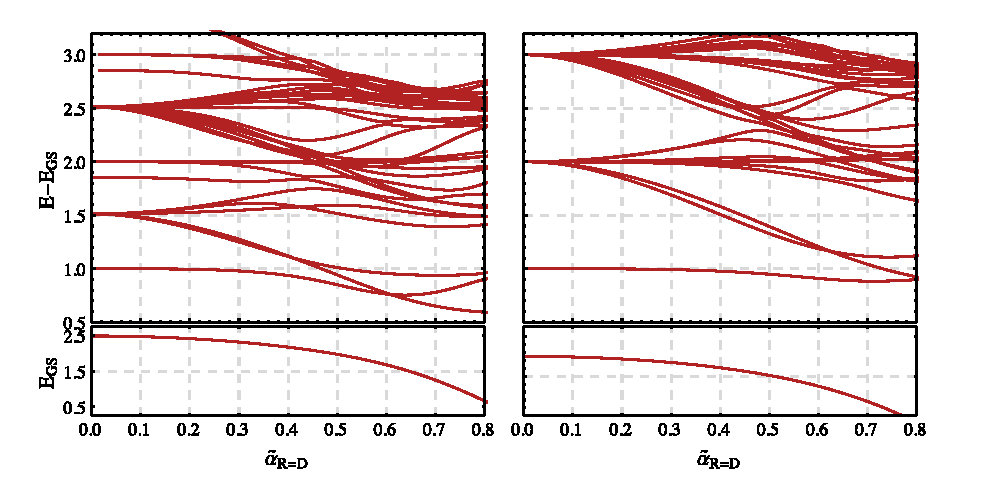
\includegraphics{SOC/Figures/RashbaDresselhausSpectrum}
\caption[Spectrum of states with even total angular momentum magnetic quantum number $J_z=0,2,\dots$ for the equal-weight Rashba-Dresselhaus coupling]{\label{fig:R=DExcitationSpectrum} 
Spectrum of states with even total angular momentum magnetic quantum number $J_z=0,2,\dots$ for the equal-weight Rashba-Dresselhaus SOC~\eqref{eq:R=D}. The left figure shows the energies with negative scattering length $\tilde{a}=-1$. The right figure shows the results in the unitary limit $|\tilde{a}|\rightarrow\infty$. The spectrum is symmetric about $\tilde{\alpha}_{R=D}=0$.} 
\end{figure}


\section{Conclusions}

In this chapter we have nonperturbatively calculated the spectrum of interacting two-particle systems with realistic spin-orbit couplings when the trapping potential cannot be ignored.  Matrix elements of a short-range pseudopotential and three types of spin-orbit coupling were determined analytically in a basis of the total angular momentum eigenstates of the interacting two-body problem without SOC. With the analytic matrix elements, exact diagonalization of the Hamiltonian within a finite basis was possible.

Our energy calculations were performed in a basis truncated in a consistent way by including all states below an energy cutoff. The resulting spectra show good convergence except in the case where the two-body interaction generates a small positive scattering length. In this regime coupling of the ground state to higher relative-coordinate excited states dominates and convergence in the cutoff parameter $E_{\text{max}}$ was numerically intractable. We are currently investigating alternative methods to deal with this issue. In the limit of weak SOC we have compared our results to the perturbative calculations of \cite{PhysRevA.89.033606} and found good agreement. We also observed that although the ground state does not couple strongly to center-of-mass excitations, their inclusion is crucial for the excited state spectrum.  The relatively weak center-of-mass coupling of the ground state, however, suggests that cold atoms with SOC can be used as a surrogate system to probe properties of two-body spin-orbit couplings, e.g., the parity-violating weak interaction in nuclear systems. 

We provided plots of a variety of spectra calculated with Weyl, Rashba, and equal weight Rashba-Dresselhaus couplings.  Although in this thesis we show spectra only within certain subspaces of conserved angular momentum quantum numbers, the approach presented is fully capable of generating results for all possible states. Larger SO-coupling constants are also accessible with larger basis sizes. The general method can easily be adapted to calculate energies for bosonic systems, or to new forms of SOC such as the recently proposed spin-orbital angular momentum coupling \cite{2014arXiv1411.1737S}.  

Using the eigenvectors of the truncated basis Hamiltonian, we also explored the effect of parity violation on the system. In particular we show how the SOC induces mixing of the positive- and negative-parity subspaces for the ground state. Without a two-body interaction, the ground state preferentially projects onto negative parity basis states even for modest SOC strength. The short-range interaction was seen to suppress this mixing, especially when the scattering length is positive.

A natural extension of this work is to consider three particles within a trap.  Because of the complex spectrum that is associated with three-body physics at the unitary limit (e.g., Efimov states, limit cycles, etc.), the spectrum under the influence of an external SOC is expected to be quite rich.  Couplings between the center-of-mass and relative motion due to the SOC present a potential challenge to traditional few-body techniques, such as the Faddeev equations, which work only within the relative coordinates.  However, in our two-body calculations we found that the coupling of the ground state to the c.m. motion is weak. If this is also true in the three-body case, then to a good approximation we can ignore the c.m. motion and utilize existing few-body techniques with little or no modification.  

%\chapter{\label{chap:SOC}Energy Spectra of Two Interacting Fermions with Spin-Orbit Coupling in a Harmonic Trap}

%\begin{abstract}
%We explore the two-body spectra of spin-$1/2$ fermions in isotropic harmonic traps with external spin-orbit potentials and short range two-body interactions. Using a truncated basis of total angular momentum eigenstates, nonperturbative results are presented for experimentally realistic forms of the spin-orbit coupling: a pure Rashba coupling, Rashba and Dresselhaus couplings in equal parts, and a Weyl-type coupling. The technique is easily adapted to bosonic systems and other forms of spin-orbit coupling.
%\end{abstract}

Cold atomic gases with parity-violating spin-orbit coupling (SOC) have recently been an area of intense interest because of the potential to simulate interesting physical systems with precisely tunable interactions \cite{nature11841}. In condensed-matter and atomic physics, spin-orbit couplings\footnote{In these fields, spin-orbit coupling conventionally refers to operators which couple spin with momentum, as opposed to the more restrictive use in nuclear and atomic physics where there term specifically refers to a parity-conserving $\vec{\ell}\cdot \vec{s}$ interaction.}\ are essential for many exotic systems such as topological insulators \cite{das2013engineering,PhysRevLett.105.255302}, the quantum spin Hall effect \cite{nature12185}, and spintronics \cite{RevModPhys.76.323}. The experimental setup which induces spin-orbit coupling is intimately related to simulation of synthetic gauge fields \cite{RevModPhys.83.1523,hamner2014dicke,Lin:2009zzb,Bermudez:2011db}. Because these couplings are parity violating, they potentially play similar roles within nuclear systems that undergo parity-violating transitions due to the nuclear weak force.  Atomic gases provide an excellent testing ground both to explore universal behavior of these real life systems and to create new types of spin-orbit coupling which are not yet known to exist (or have no solid-state analog) in other materials but are interesting in their own right. Further, these experiments can be performed in an environment with few or no defects and impurities.

Spin-orbit coupling was first realized in a Bose condensate of $^{87}$Rb \cite{nature09887} and extended shortly after to Fermi gases of $^{40}$K \cite{PhysRevLett.109.095301} and $^6$Li \cite{PhysRevLett.109.095302}. These spin-orbit interactions are `synthetic' in the sense that a subset of the hyperfine states stand in as virtual spin states. A particularly interesting consequence of this is the possibility of studying systems with synthetic spin-$1/2$ spin-orbit interactions but bosonic statistics \cite{PhysRevA.68.063612,nature09887}. From another point of view, the couplings are equivalent to applying external electromagnetic forces via synthetic gauge couplings on the physically uncharged particles in the gas \cite{Lin:2011,PhysRevLett.107.255301}. It has also been conjectured that these systems could be used to physically simulate lattice gauge theories \cite{Bermudez:2010da,Mazza:2011kf}.  Spin-orbit couplings in solid-state systems arise in two-dimensional (2D) systems (Rashba and Dresselhaus types, described in Sec.~\ref{sec:Hamiltonian}), but recently an experimental setup has been proposed that can simulate the Weyl-type SOC which is fundamentally three dimensional \cite{PhysRevLett.108.235301}.

Spin-orbit couplings are also of interest from the perspective of few-body physics where they arise in a variety of fields, e.g., the weak nuclear interactions governing proton-proton scattering \cite{Haxton:2013aca,deVries:2014vqa}. Because the spin-orbit coupling is long range, it can significantly modify both the threshold scattering behavior and the spectrum of two-body systems \cite{PhysRevA.86.042707}. For low-energy scattering, Duan \textit{et al.} \cite{PhysRevA.87.052708} showed analytically that parity-violating SOC leads to the the spontaneous emergence of handedness in outgoing states, a finding later confirmed in \cite{PhysRevA.91.022706}. Even in the presence of a repulsive two-body interaction, an arbitrarily weak SOC has been shown to bind dimers \cite{PhysRevB.83.094515}. For three-particle systems, a new type of universality is conjectured to occur for bound trimers with negative scattering length \cite{PhysRevLett.112.013201}. 

Few-atom systems undergoing SOC within trapping potentials have also been explored. For example, the spectrum of particles within a trap with an external SOC of the Weyl type (but no relative interaction) has been theoretically determined \cite{anderson2013}. The Rashba SOC with two-particle systems interacting via short-ranged interactions was investigated perturbatively in \cite{PhysRevA.89.033606}, where it was shown that the leading order corrections due to the SOC and short-range interaction are independent when the scattering length is equal for all channels.  In one dimension, the spectrum for this type of system has been calculated when the SOC consists of equal parts Rashba and Dresselhaus interactions \cite{guan2014energy}. Information learned from trapped systems augments that from scattering experiments while also being relevant to interesting phenomena in trapped many-body systems with SOC such as solitons \cite{DarkSolitons,PhysRevA.87.013614} or novel phase diagrams \cite{PhysRevLett.107.270401}.


In all these calculations, the emergent spectrum is rich and complex, offering new insights into few-body behavior.  Our objective is to provide some additional insight into two-body physics of Fermi gases with spin-orbit interactions in the presence of both three-dimensional trapping potentials and short-ranged two-body interactions, which are necessarily present in dilute cold-atom experiments. Our approach is to numerically diagonalize the Hamiltonian within a suitably truncated basis, and is thus nonperturbative in nature. Eigenstates of the interacting Hamiltonian without SOC are used for the basis. Section~\ref{sec:Hamiltonian} introduces the specific forms of spin-orbit coupling and two-body interactions which we consider. The general method is detailed in Sec.~\ref{sec:Weyl} for the simplest SOC.  In the remaining Secs.~\ref{sec:Rashba}-\ref{sec:R=D} we study the spectra of additional spin-orbit couplings in order of increasing computational complexity.

\section{\label{sec:Hamiltonian}Hamiltonian for Spin-orbit Couplings with Contact Interactions}

In this chapter we simply refer to our systems by their `spin' degrees of freedom and use the standard notation for spin quantum numbers. We consider three different types of spin-orbit coupling. The form of spin-orbit coupling realized in experiments is a linear combination of the Rashba \cite{0022-3719-17-33-015} and linear Dresselhaus \cite{PhysRev.100.580} types,
\begin{align}
V_{R}&\equiv\alpha_R (\sigma_x k_y-\sigma_y k_x) \label{eq:Rashba},\\
V_{D}&\equiv\alpha_D (\sigma_x k_y+\sigma_y k_x) \label{eq:Dresselhaus},
\end{align} 
which were originally recognized in two-dimensional solid-state systems. In a 2D system, these form a complete basis for spin-orbit couplings linear in momentum. Note that some references use the alternate definitions $V_R\propto  (\sigma_x k_x+\sigma_y k_y) $ and $V_D\propto  (\sigma_x k_x-\sigma_y k_y) $ which are equivalent up to a pseudospin rotation.  For solids, these parity-violating interactions are allowed only in the absence of inversion symmetries. Rashba-type SOC typically arises in the presence of applied electric fields or in 2D subspaces such as the surfaces of materials where the boundary breaks the symmetry. Dresselhaus couplings were first studied in the context of bulk inversion asymmetry, when the internal structure leads to gradients in the microscopic electric field. 

To date, experiments have produced only SOC potentials in which the Rashba and Dresselhaus terms appear with equal strength (also known as the ``persistent spin-helix symmetry point'' \cite{PhysRevLett.97.236601}), 
\begin{equation}
\label{eq:R=D}
V_{R=D}\equiv\alpha_{R=D}\sigma_x k_y.
\end{equation} 
After a pseudospin rotation, this potential can be seen as a unidirectional coupling of the pseudospin and momentum along a single axis. A proposal for tuning the ratio $\alpha_R/\alpha_D$ has been given in \cite{PhysRevA.84.025602}.  An experimental setup which gives the simple three-dimensional Weyl coupling,
\begin{equation}\label{eq:Weyl}
V_{W}\equiv\alpha_W \vec{k}\cdot\vec{\sigma},
\end{equation}
has also been proposed in \cite{PhysRevLett.108.235301} and \cite{PhysRevLett.111.125301}. 

In the following sections we calculate the spectra of two particles with a short-range two-body interaction, an isotropic harmonic trapping potential and spin-orbit coupling. The single particle Hamiltonian is 
\begin{equation}\label{eq:shortRangeInteraction}
H_1=\frac{\hbar^2 k^2}{2m}+\frac{1}{2}m\omega^2 r^2 + V_{\text{SO}}.
\end{equation}
For the spin-orbit term $V_{\text{SO}}$, we consider equal Rashba and Dresselhaus~\eqref{eq:R=D}, pure Rashba~\eqref{eq:Rashba}, and Weyl~\eqref{eq:Weyl} spin-orbit couplings  because these are generally considered to be experimentally feasible.

We assume that the range of interaction between particles is small compared to the size of the oscillator well.  The relative interaction between the particles can then be approximated as a regulated $s$-wave contact interaction, which in momentum space (as a function of relative momentum) is given by
\begin{equation}
\frac{4\pi \hbar^2}{m}a(\Lambda)\ .
\end{equation}
Here the argument $\Lambda$ refers to some cutoff scale and $a(\Lambda)$ is some function of the cutoff and physical scattering length $a_{\text{phys}}$.  The exact form of this function depends on the type of regulator used and is not relevant for this work; the only constraint is that $a(\Lambda)$ reproduce the physical scattering length given by the scattering $T$ matrix at threshold, $T(E=0)=4\pi\hbar^2 a_{\text{phys}}/m$ \cite{taylor2000}. In the limit $\Lambda\rightarrow \infty$ the spectrum of two particles in an oscillator well (without external spin-orbit interaction) was solved by Busch \textit{et al.} \cite{Busch} using the method of pseudopotentials.  In Ref.  \cite{Luu:2006xv} the solution for general $\Lambda$ was given using a Gaussian regulator, which in the limit $\Lambda\rightarrow\infty$ recovered the Busch \textit{et al.} solution.  For our work below we use the eigenstates and eigenvalues of this two-particle system given in Ref. \cite{Busch}.

\section{\label{sec:Weyl}Weyl Coupling}
We tackle the Weyl form first because of its mathematical and numerical simplicity. In the absence of the two-body interaction, this problem was treated in Ref. \cite{anderson2013}. Our approach is to determine the matrix elements of the SOC in an appropriate basis. The eigenvalue is then solved numerically at the desired precision by choosing an appropriately large truncated basis of harmonic oscillator (HO) eigenstates.

As usual, the two-body problem is best approached in the dimensionless Jacobi coordinates
\begin{equation}
R=\frac{r_1+r_2}{\sqrt{2}b}, \qquad r=\frac{r_1-r_2}{\sqrt{2}b}
\end{equation}
and the corresponding conjugate momenta $q,Q$ representing the relative and total momenta. For an isotropic harmonic oscillator, distances can be expressed in terms of the ground-state length scale $b=\sqrt{\hbar/m\omega}$ and energies will be similarly measured in units of $E_0=\hbar\omega$. We also define the spin operators
\begin{equation}
\vec{\sigma}\equiv\vec{\sigma}_1-\vec{\sigma}_2, \qquad \vec{\Sigma}\equiv\vec{\sigma}_1+\vec{\sigma}_2.
\end{equation}

With these definitions, the two-body Hamiltonian can be nondimensionalized and separated into relative and center-of-mass (c.m.) parts,
\begin{equation}\label{eq:WeylHamiltonian}
\frac{1}{\hbar\omega}H=\left(h_{0,\text{rel}}+\frac{\tilde{\alpha}_W}{\sqrt{2}} \vec{q}\cdot\vec{\sigma} + \sqrt{2}\pi \tilde{a}(\Lambda) \delta^{(3)}(r)\right)+\left(h_{0,\text{c.m.}}+\frac{\tilde{\alpha}_W}{\sqrt{2}} \vec{Q}\cdot\vec{\Sigma} \right),
\end{equation}
where $h_{0,\text{rel}}=r^2/2$ and $h_{0,\text{c.m.}}=R^2/2$. Notably, the spin-orbit coupling appears in both terms.  The tilde over the coupling constants indicates that they are dimensionless, related to the original coupling constants by e.g., $\tilde{\alpha}_W=\alpha_W/(\hbar\omega b)$. Similarly the scattering length is made dimensionless by dividing out the oscillator length, $\tilde{a}=a/b$. Throughout the remainder of this chapter we will refer to dimensionless eigenvalues of $H/\hbar\omega$ as the energies of the system.

%We point out that the relative-coordinate spin-orbit term in Eq.~\eqref{eq:WeylHamiltonian} is exactly of the form that appears in weak-interaction parity-violating proton-proton scattering \cite{Haxton:2013aca,deVries:2014vqa}.  Aside from Coulomb contributions, the $^1S_0$ channel of proton-proton scattering has a scattering length that is an order of magnitude larger than its effective range.  The parity-conserving part of the nuclear potential could therefore be represented by the contact interaction in Eq.~\eqref{eq:WeylHamiltonian}.  The CM spin-orbit term (i.e. the last term in Eq.~\eqref{eq:WeylHamiltonian}) spoils this analogy. However, we will show later that the effect of this term on the ground state is negligible. 

\begin{figure}
\centering
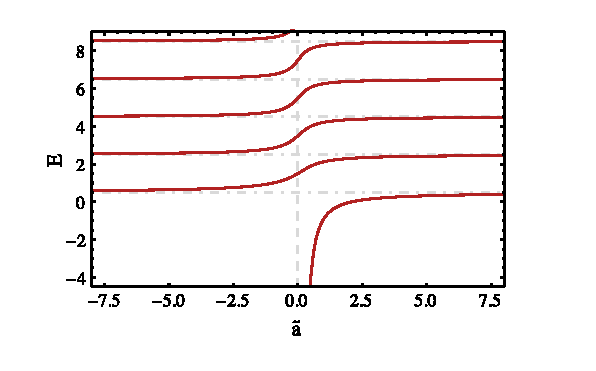
\includegraphics[scale=1.2]{SOC/Figures/BuschSpectrum}
\caption[Spectrum of the two-body contact interaction Hamiltonian as a function of $\tilde a$]{\label{fig:BuschSpectrum} Spectrum of the two-body contact interaction Hamiltonian as a function of $\tilde a$. The horizontal lines indicate the dimensionless energy eigenvalues in the unitary limit $|\tilde{a}|\rightarrow\infty$.} 
\end{figure}

Eigenstates of two particles with a short-range interaction in a harmonic oscillator trapping potential form a convenient basis for these calculations. These basis functions were first derived in \cite{Busch} for the isotropic case considered here, and the more general case of an anisotropic trap has been explored in \cite{PhysRevA.74.022712}. The dependence of the energy spectrum on the scattering length $a$ is shown in Fig.~\ref{fig:BuschSpectrum} for reference. Qualitatively, the effect of the short-range interaction is to shift the harmonic oscillator energies by $\pm \hbar\omega$ as the scattering length goes to $\pm \infty$. For positive scattering length, there is also an additional negative-energy dimer state.

We choose the particular coupling scheme of angular momentum eigenstates,
\begin{equation}\label{eq:basisStates}
\ket{n(ls)j;NL;(jL)J},
\end{equation}
which simplify the matrix elements for the relative-coordinate operators. Here $n$ and $l$ refer to the principal and orbital angular-momentum quantum numbers of the two-particle system in the relative coordinates. $N$ and $L$ refer to the analogous numbers in the center-of-mass frame. The total spin of the two spin-$1/2$ particles is denoted by $s = s_1 + s_2$ and may be either 0 or 1. First $s$ and $l$ to make angular momentum $j$, which is then recoupled with the c.m. angular momentum $L$ to make the state's total angular momentum $J$. Because all terms in the Hamiltonian~\eqref{eq:WeylHamiltonian} are scalars, the interaction is independent of $J_z$ and so we omit this quantum number for clarity. Due to Pauli exclusion, $l + s$ must be even to enforce antisymmetry under exchange of the particles.

For $l\neq0$ the states~\eqref{eq:basisStates} are identical to the well known harmonic oscillator, with $n$ and $l$ ($N$ and $L$) indicating the relative (center-of-mass) HO quantum numbers. We use the convention that $n,N=0,1,2,\dots$, and therefore $E=2n+l+2N+L+3$. The short range interaction~\eqref{eq:shortRangeInteraction} modifies the $l=0$ states and their spectrum. The principal relative quantum number $n$ for these states is obtained by solving the transcendental equation
\begin{equation}\label{eq:eigenvalueEqn}
\sqrt{2}\frac{\Gamma(-n)}{\Gamma(-n-1/2)}=\frac{1}{\tilde{a}}
\end{equation}
and is no longer integer valued. For the relative-coordinate part of the $l=0$ wave function,
\begin{align}
\phi(r)&=\frac{1}{2\pi^{3/2}}A(n)\Gamma(-n)U(-n,3/2,r^2)e^{-r^2/2}, \label{eq:BuschWF}\\
A(n)&=\left(\frac{\Gamma(-n)[\psi_0(-n)-\psi_0(-n-1/2)]}{8 \pi^2 \Gamma(-n-1/2)}\right)^{-1/2},
\end{align}
where $U(a,b,x)$ is Kummer's confluent hypergeometric function and $\psi_0(x)=\Gamma'(x)/\Gamma(x)$ is the digamma function. A derivation of the normalization factor $A(n)$ is given in the Appendix.

Standard angular momentum algebra can be used to determine the matrix elements of the two spin-orbit coupling terms; we follow the conventions of \cite{Edmonds}. For Weyl SOC of two spin-$1/2$ fermions, the matrix elements of the coupling in the relative momentum are
\begin{equation}\label{eq:WeylRel}\begin{split}
\bra{n'(l's')j';N'L';(j'L')J'}\vec{q}&\cdot\vec{\sigma} \ket{n(ls)j;NL;(jL)J}  \\
=&\delta_{N,N'}\delta_{L,L'}\delta_{j,j'}\delta_{J,J'}(-1)^{l+s'+j}\frac{3}{\sqrt{2}}\sixj{j}{s'}{l'}{1}{l}{s} (s'-s)\braket{n'l' || q || n l}.
\end{split}
\end{equation}
To preserve anti-symmetry of the two-particle system, the relative momentum term in the Weyl SOC must couple states with relative angular momentum $l$ to $l\pm 1$, leaving $l+s$ even but changing the parity.

For basis states with both $l,l'\neq0$, reduced matrix elements of the momentum operator are calculated between pure harmonic oscillator states,
% Could do away with some constants in favor of the 3-j coefficient
\begin{align}
\braket{n'l' || q || n l}=&(-1)^{l'}(-1)^{\frac{l+l'+1}{2}}\sqrt{\frac{2(2l+1)(2l'+1)}{(l+l'+1)}}\braket{n'l'0| (-i \nabla_0) | n l 0} \\
\begin{split} =& i(-1)^{l}\sqrt{\frac{l+l'+1}{2}}\sqrt{n!n'!\Gamma(n+l+3/2)\Gamma(n'+l'+3/2)} \\ 
&\times\sum_{m,m'=0}^{n,n'} \left\{
     \begin{array}{lr}
       \frac{(-1)^{m+m'}\left[2m\Gamma\left(m+m'+1+\frac{l+l'}{2}\right)-\Gamma\left(m+m'+1+\frac{l+l'}{2}\right)\right]}{m!m'!(n-m)!(n'-m')!\Gamma(m+l+3/2)\Gamma(m'+l'+3/2)} & \text{if}\: l'=l-1 \\
        \frac{(-1)^{m+m'+1}\left[(2m+2l+1)\Gamma\left(m+m'+1+\frac{l+l'}{2}\right)-\Gamma\left(m+m'+1+\frac{l+l'}{2}\right)\right]}{m!m'!(n-m)!(n'-m')!\Gamma(m+l+3/2)\Gamma(m'+l'+3/2)} & \text{if}\: l'=l+1 \\
       0 & \text{otherwise}
     \end{array}
   \right.
   \end{split}
\end{align}
If $l=1$ and $l'=0$ or vice versa, reduced matrix elements between one modified wave function of the form~\eqref{eq:BuschWF} and one pure harmonic oscillator state are needed. These are given by
\begin{align}
\braket{n l=0 || q || n' l'=1}=-i A(n) \sqrt{\frac{\Gamma(n'+5/2)}{2\pi^3 n'!}}\frac{2n-2n'-1}{2(n'-n)(1+n'-n)}
\end{align}
and its Hermitian conjugate.

Our choice of basis makes the relative matrix elements~\eqref{eq:WeylRel} simple at the cost of complicating the center-of-mass term. We take the approach of expanding the states~\eqref{eq:basisStates} in the alternate coupling scheme,
\begin{equation}\label{eq:basisStates2}
\ket{n(ls)j;NL;(jL)J}=(-1)^{l+s+L+J}\sqrt{2j+1}\sum_{\mathcal{J}}\sqrt{2\mathcal{J}+1}\sixj{l}{s}{j}{L}{J}{\mathcal{J}}\ket{nl;N(Ls)\mathcal{J};(l\mathcal{J})J}.
\end{equation}
Using this notation, the matrix elements can be written
\begin{equation}\begin{split}
\bra{n'(l's')j';N'L';(j'L')J'}&\vec{Q}\cdot\vec{\Sigma} \ket{n(ls)j;NL;(jL)J} = \delta_{n,n'}\delta_{l,l'}\delta_{J,J'}\delta_{s,1}\delta_{s1,1}   6 (-1)^{L} \\
&\hspace{-2cm}\times\braket{N'L'|| \vec{Q} || NL} \sum_{\mathcal{J}}(-1)^\mathcal{J} (2\mathcal{J}+1)\sixj{l}{1}{j'}{L'}{J}{\mathcal{J}}\sixj{l}{1}{j}{L}{J}{\mathcal{J}}\sixj{\mathcal{J}}{1}{L'}{1}{L}{1}.
\end{split}
\end{equation}
Again, the reduced matrix element of the center-of-mass momentum changes the parity by connecting states with $\Delta L=\pm1$. Matrix elements are nonzero only for $\Delta s=0$ because the antisymmetry of the spatial wave function depends only on $l$, which does not change. We also note that the c.m. term does not affect states with singlet spin wave functions ($s=0$).


\begin{figure}
\centering
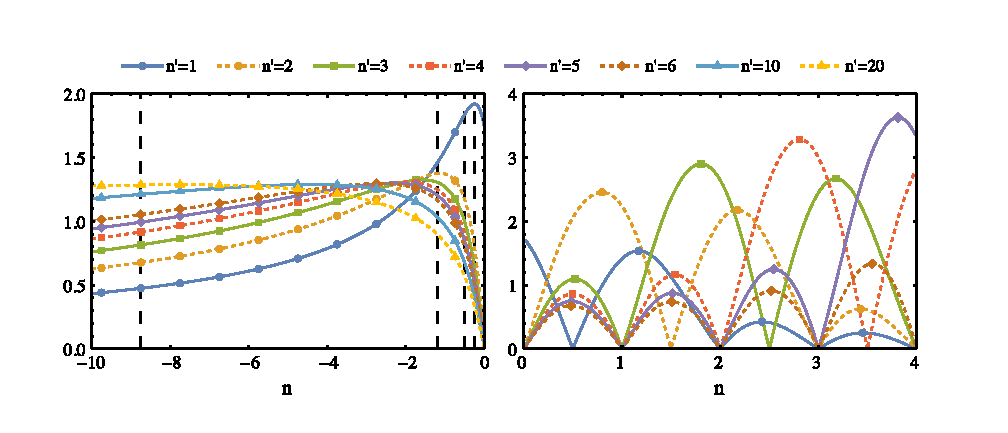
\includegraphics{SOC/Figures/MatrixElts}
\caption[Coupling of ground state to $l=1$ states for the Weyl spin-orbit Hamiltonian]{\label{fig:matrixElts}Absolute value of the matrix elements $|\bra{n'(11)0;00;(00)0}\vec{\sigma}\cdot\vec{q}\ket{n(00)0;00;(00)0}|$ between the ground state and $l=1$ excited states. The horizontal axis is the principal quantum number of the ground state obtained by solving~\eqref{eq:eigenvalueEqn}. From left to right, the vertical lines on the negative axis indicate the values obtained for $\tilde{a}=1/4$, $\tilde{a}=1$, $\tilde{a}=\pm\infty$, and $\tilde{a}=-1$, respectively.} 
\end{figure}

Using these matrix elements, we calculated the spectrum of the two interacting particles with Weyl spin-orbit coupling. Our calculations are performed by numerically diagonalizing in a truncated basis of the harmonic oscillator states~\eqref{eq:basisStates}, where a cutoff $2N+L+\nobreak 2n+\nobreak l+ \nobreak3\leq\nobreak E_{\text{max}}$ is set high enough that the eigenvalues of the matrix have converged to the desired accuracy.  

\begin{figure}
\centering
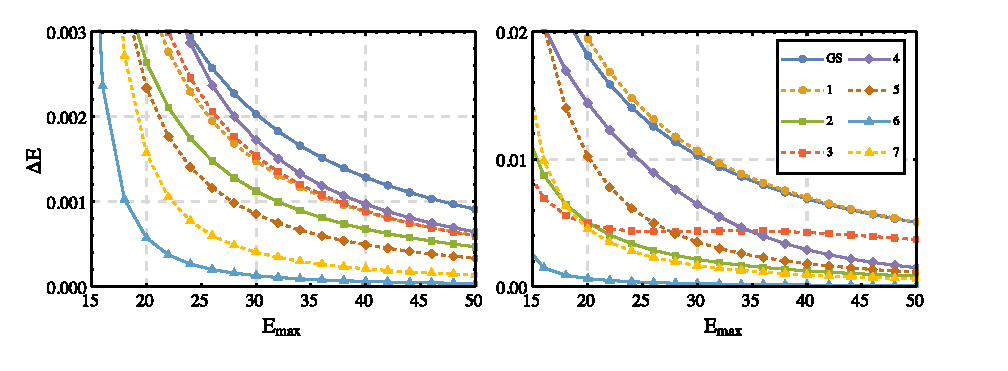
\includegraphics{SOC/Figures/WeylConvergence}
\caption[Convergence of the energy eigenvalues for the Weyl spin-orbit coupling]{\label{fig:WeylConvergence}  A convergence plot giving the change in energy eigenvalue, $\Delta E$, for the lowest eight energy levels when a shell is added as a function of $E_{\text{max}}$.  The left figure shows convergence for $\tilde{a}=-1$ and $\tilde{\alpha}_W=0.5$. In the right panel  we show $\tilde{a}=1$ and $\tilde{\alpha}_W=0.5$, demonstrating that convergence of the states with large negative $n$ is poor.} 
\end{figure}

This approach converges well only when the ground-state energy is not too low. In particular, for $a$ positive but very small the principal quantum number of the ground state is increasing from negative infinity as seen in Fig.~\ref{fig:BuschSpectrum}. From Fig.~\ref{fig:matrixElts}, we can see that as $n$ becomes more negative, the principal quantum number of the dominant matrix element is also increasing. Because convergence of any energy level requires a cutoff much larger than the energy of the most strongly coupled states, a sufficiently high $E_{\text{max}}$ to ensure an accurate ground-state energy becomes infeasible for small positive $a$. For excited states, $n$ is always positive and matrix elements with similar $n$ always dominate. The strength of the matrix elements follows a similar qualitative behavior for the spin-orbit couplings treated in the following sections where the same issues recur. 

\begin{figure}
\centering
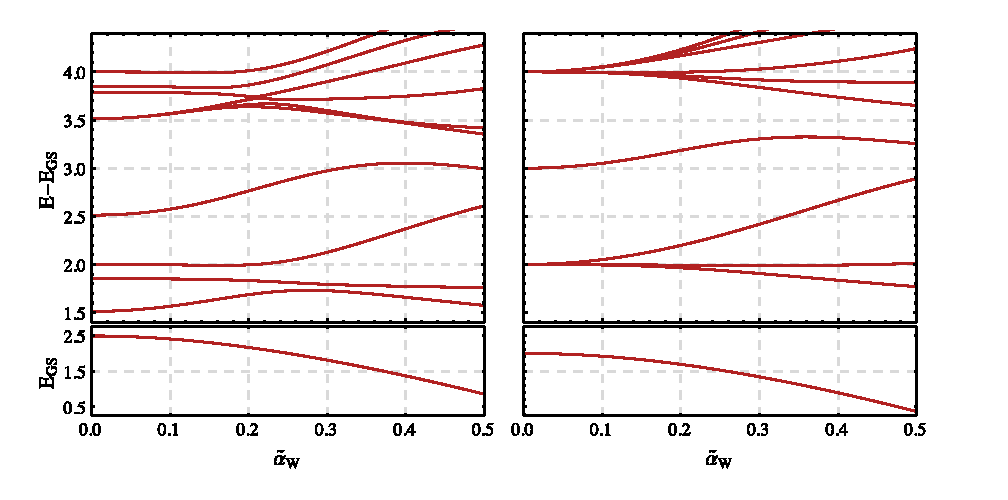
\includegraphics{SOC/Figures/WeylSpectrum}
\caption[Spectrum of states with $J=0$ for Weyl spin-orbit coupling]{\label{fig:WeylSpectrum}  Spectrum of states with total angular momentum $J=0$ for the dimensionless Hamiltonian~\eqref{eq:WeylHamiltonian}. The bottom left figure shows the ground-state energy for $\tilde{a}=-1$ as a function of $\tilde{\alpha}_W$; above are the first few excitation energies. The right figure shows the results in the unitary limit of the two-body interaction, $|\tilde{a}|\rightarrow\infty$. The spectrum is symmetric about $\tilde{\alpha}_W=0$.} 
\end{figure}

As a result, convergence of the ground state is actually slower than that for nearby excited states. Furthermore, our approach gives the fastest convergence when $a$ is not small and positive. We compare the rate of convergence of the $\tilde{a}=-1$ and $\tilde{a}=1$ spectra in Fig.~\ref{fig:WeylConvergence} to demonstrate the dependence of convergence on the matrix truncation. The actual energy spectrum is shown in Fig.~\ref{fig:WeylSpectrum}. 

\begin{figure}
\centering
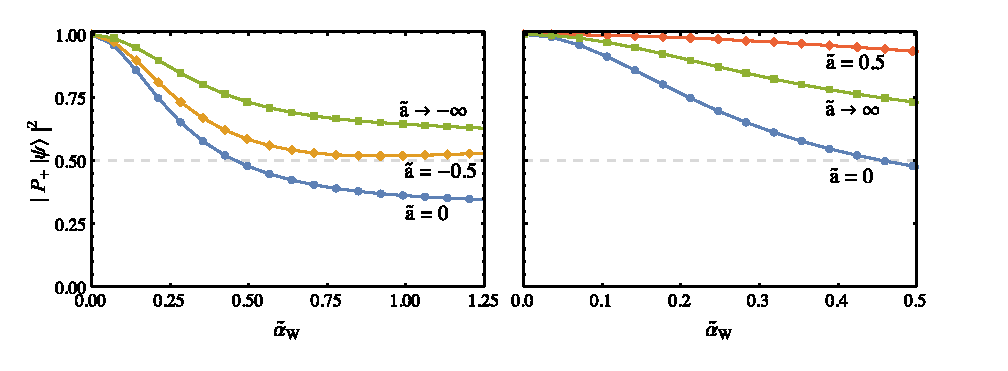
\includegraphics{SOC/Figures/Projections}
\caption[Parity projection of the Weyl spin-orbit coupling ground state]{\label{fig:Projections} For different values of the two-body coupling strength $\tilde{a}$, we show the magnitude of the ground state projected onto even parity basis states as a function of the SOC strength. This is given by $\big|  P_+\ket{\psi_{\text{GS}}}\big|^2=\big| (1- P_-)\ket{\psi_{\text{GS}}}\big|^2$, where $P_+$ ($P_-$) is the projection operator onto the positive\nobreak- (negative\nobreak-) parity basis states. The left figure shows negative $\tilde{a}$, while the right shows positive $\tilde{a}$. Note that the limits $\tilde{a}\rightarrow\pm\infty$ are physically identical.}
\end{figure}

One consequence of parity violation in this system is that the eigenstates are mixtures of the even- and odd-parity basis states described by Eq.~\eqref{eq:basisStates}. In Fig.~\ref{fig:Projections} we visualize how these subspaces are mixed in the ground state as the SOC strength increases. For the noninteracting system, $\tilde{a}=0$, more than half of the ground state projects onto negative-parity states even at fairly small values of $\tilde{\alpha}_W$. However, we see that the short-range interaction reduces this effect. With negative $\tilde{a}$, the mixing of the negative-parity states is suppressed as the strength of the two-body interaction increases. When $\tilde{a}$ is positive the effect is more striking. Mixing with negative-parity states is most strongly suppressed for small positive values of $\tilde{a}$, while the projection onto these states increases for larger positive values. The admixture is qualitatively the same when considering other forms of SOC as described in the following sections.

\section{\label{sec:Rashba}The Pure Rashba Coupling}

In order to find the matrix elements of the pure Rashba coupling given in~\eqref{eq:Rashba}, we first note that it can be written as a spherical tensor
\begin{equation}
V_{R}=i\sqrt{2}\:\alpha_R \left[ k \otimes \sigma \right]_{10}.
\end{equation}
We therefore have the two-body Hamiltonian
\begin{equation}\label{eq:RashbaHamiltonian}
\frac{1}{\hbar\omega}H=\left(h_{0,\text{rel}}+i \tilde{\alpha}_R  \left[ \vec{q} \otimes \vec{\sigma} \right]_{10} + \sqrt{2}\pi \tilde{a}(\Lambda) \delta^{(3)}(r)\right)+\left(h_{0,\text{c.m.}}+i \tilde{\alpha}_R [ \vec{Q}\otimes \vec{\Sigma} ]_{10} \right).
\end{equation}

Because the spin-orbit coupling is now a $k=1$ tensor rather than a scalar operator, the total angular momentum $J$ is no longer conserved. Additionally, the matrix elements now depend on the quantum number $J_z$ (which is conserved). For the relative-coordinate part of the SOC, some algebra gives
\begin{equation}\begin{split}
&\bra{n'(l's')j';N'L';(j'L')J'J'_z}  [ \vec{q} \otimes \vec{\sigma} ]_{10}  \ket{n(ls)j;NL;(jL)JJ_z} = \\
&\hspace{1.5cm} 6 i (-1)^{J+J'-J'_z+j'+L+1}\delta_{N,N'}\delta_{L,L'}\delta_{J_z,J'_z} \sqrt{(2J+1)(2J'+1)(2j+1)(2j'+1)} \\
 &\hspace{2.7cm} \times \threej{J'}{1}{J}{-J_z}{0}{J_z} \sixj{j'}{J'}{L}{J}{j}{1}
 \renewcommand{\arraystretch}{0.9}
 \ninej{\hphantom{l}l'\hphantom{l}}{\hphantom{l}l\hphantom{l}}{\hphantom{l}1\hphantom{l}}{s'}{s}{1}{j'}{j}{1} (s'-s) \braket{n'l' || q || n l}.
\end{split}
\end{equation}
For the center-of-mass part of the Hamiltonian we again expand the basis states in the alternate coupling scheme~\eqref{eq:basisStates2} to obtain the matrix elements
\begin{equation}\begin{split}
&\bra{n'(l's')j';N'L';(j'L')J'J'_z} [ \vec{Q} \otimes \vec{\Sigma} ]_{10}  \ket{n(ls)j;NL;(jL)JJ_z} = \delta_{n,n'}\delta_{l,l'}\delta_{J_z,J'_z}\delta_{s,1}\delta_{s',1} \\
 &\quad\times 6 i \sqrt{2}(-1)^{J+J'-J'_z+l} \sqrt{(2J+1)(2J'+1)(2j+1)(2j'+1)} \threej{J'}{1}{J}{-J_z}{0}{J_z}  \braket{N' L' || Q || N L} \\ 
 &\quad\times\sum_{\mathcal{J},\mathcal{J}'} (-1)^\mathcal{J}(2\mathcal{J}+1)(2\mathcal{J}'+1)\sixj{l}{1}{j'}{L'}{J'}{\mathcal{J}'}\sixj{l}{1}{j}{L}{J}{\mathcal{J}}\sixj{\mathcal{J}'}{J'}{l}{J}{\mathcal{J}}{1}
 \renewcommand{\arraystretch}{0.9}
 \ninej{\hphantom{l}L'\hphantom{l}}{\hphantom{l}L\hphantom{l}}{\hphantom{l}1\hphantom{l}}{1}{1}{1}{\mathcal{J}'}{\mathcal{J}}{1} .
\end{split}
\end{equation}

\begin{figure}
\centering
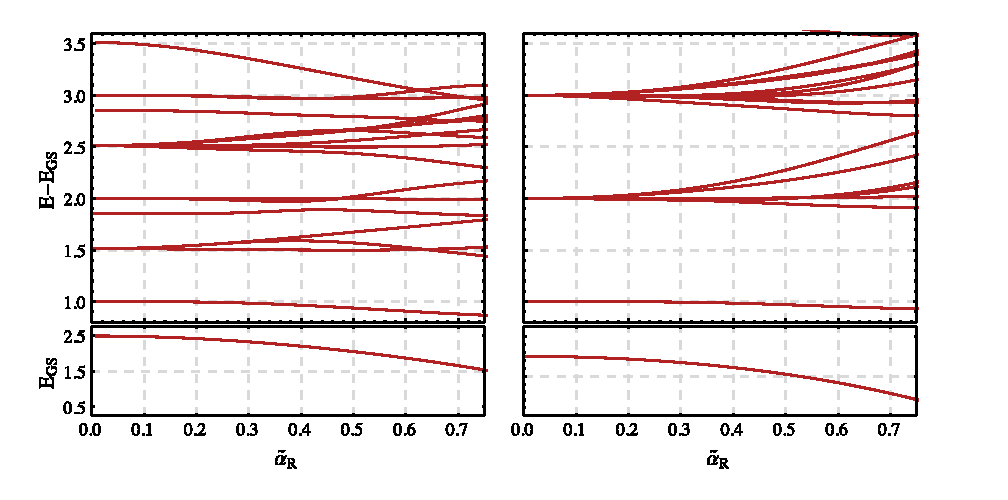
\includegraphics{SOC/Figures/RashbaSpectrum}
\caption[Spectrum of the Rashba spin-orbit coupling for $J_z=0$]{\label{fig:RashbaSpectrum}  Spectrum of states with total angular momentum quantum number $J_z=0$ for the Hamiltonian~\eqref{eq:RashbaHamiltonian}. The left figure shows the energies with negative scattering length $\tilde{a}=-1$. The right figure shows the results in the unitary limit $|\tilde{a}|\rightarrow\infty$. The spectrum is symmetric about $\tilde{\alpha}_R=0$.} 
\end{figure}


Our results for the Rashba SOC are shown in Fig.~\ref{fig:RashbaSpectrum}. Because the Rashba spin-orbit coupling is a vector operator, states of all possible $J$ must be included in any calculation and the size of the basis scales much more quickly with $E_{\text{max}}$. These spectra were computed with an $E_{\text{max}}$ of $24\hbar\omega$, for which there are approximately $36\,000$ basis states. All displayed eigenvalues of the Hamiltonian shift by less than $10^{-2}\hbar\omega$ if an additional shell of states is included.

\begin{figure}
\centering
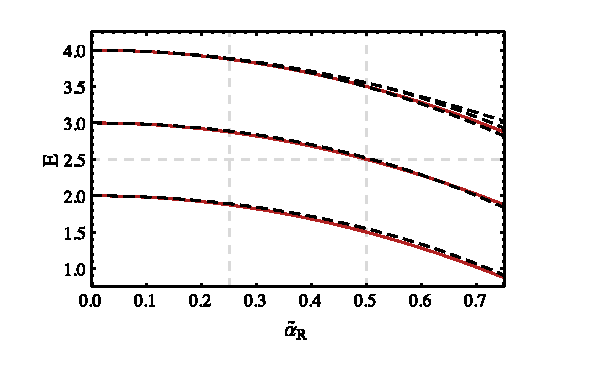
\includegraphics[scale=1.2]{SOC/Figures/PerturbativeComparison}
\caption[Comparison of the Rashba spectrum with perturbative predictions]{\label{fig:ComparisonSpectrum}Comparison of selected spectral lines (dashed black) with the perturbative predictions from \cite{PhysRevA.89.033606} (solid red) when $\tilde{a}=\infty$. }
\end{figure}

\begin{figure}
\centering
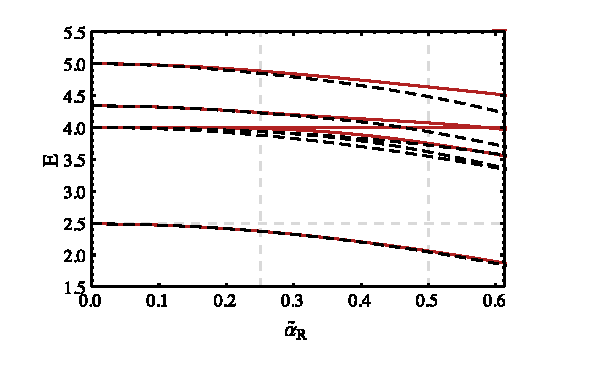
\includegraphics[scale=1.2]{SOC/Figures/ComparisonNoCM}
\caption[Effect of neglecting center of mass excitations for Rashba spin-orbit coupling]{\label{fig:ComparisonSpectrum2}  A comparison of the energy levels with (dashed black) and without (solid red) the inclusion of excitations in the c.m. coordinate for $\tilde{a}=-1$. The approximation of ignoring c.m. excitations provides very accurate results for the ground state, but not for excited states.} 
\end{figure}


This interaction was also studied perturbatively for small $\alpha_R$ in \cite{PhysRevA.89.033606}, including the possibility of a spin-dependent two-body interaction, under the assumption that center-of-mass excitations are unimportant. For the specific case of identical fermions with spin-independent scattering length considered here, they found that the first correction to the energies occurs at order $\alpha_R^2$ and is independent of the scattering length $a$. We compare their perturbative predictions, which are derived from the non-degenerate theory, with our numerical results in Fig.~\ref{fig:ComparisonSpectrum}. 

By setting all matrix elements with $N,L>0$ in the bra or ket to zero, we also explored the approximation of ignoring center-of-mass excitations. Fig.~\ref{fig:ComparisonSpectrum2} shows that this is very accurate for the ground state, but less accurate for excited states. Suppression of the c.m. coordinate has a similar effect for the SOCs considered in Secs.~\ref{sec:Weyl} and~\ref{sec:R=D}. We also note that in the case of small positive $a$, the landscape of low-lying excited states is dominated by center-of-mass excitations. When $a\rightarrow0^+$ in the absence of spin-orbit coupling, there are an infinite number of states with nonzero c.m. quantum numbers whose energies lie between the ground state and the first relative-coordinate excitation.


\section{\label{sec:R=D}Equal-Weight Rashba-Dresselhaus Spin-Orbit Coupling}

Experiments have thus far realized only the effective Hamiltonian with equal strength Rashba and Dresselhaus couplings in the form~\eqref{eq:R=D}. Energy levels of the two-body system in the one-dimensional equivalent of this Hamiltonian with the additional magnetic field couplings present in experimental realizations have been calculated in \cite{guan2014energy}. Here we treat the problem in three dimensions.

This is also the most computationally difficult of the three cases. When decomposed into spherical tensors, the interaction~\eqref{eq:Dresselhaus} becomes
\begin{equation}
V_D=i\,\alpha_D \left( \left[ k \otimes \sigma \right]_{2,-2}- \left[ k \otimes \sigma \right]_{2,2}\right),
\end{equation}
and the two-particle Hamiltonian in the presence of equal strength Rashba and Dresselhaus SOC is given by~\eqref{eq:RashbaHamiltonian} with $\alpha_R\rightarrow \alpha_{R=D}$ plus the additional spin-orbit terms
\begin{equation}\label{eq:DresselhausHamiltonian}
\Delta H= \frac{i \tilde{\alpha}_{R=D}}{\sqrt{2}}\left(  \left[ \vec{q} \otimes \vec{\sigma} \right]_{2,-2} -  \left[ \vec{q} \otimes \vec{\sigma} \right]_{2,2} +[ \vec{Q} \otimes \vec{\Sigma} ]_{2,-2} -  [ \vec{Q} \otimes \vec{\Sigma} ]_{2,2} \right).
\end{equation} 
Yet again the number of basis states with nonzero matrix elements has increased; no angular momentum quantum numbers are conserved. The only remaining selection rule will be that the interaction does not change the total magnetic quantum number $J_z$ between even and odd. 

Using the same approach as in the previous sections, the matrix elements of the relative Dresselhaus term are
\begin{equation}\begin{split}
&\bra{n'(l's')j';N'L';(j'L')J'J'_z} \frac{i \tilde{\alpha}_{R=D}}{\sqrt{2}}\left(  \left[ \vec{q} \otimes \vec{\sigma} \right]_{2,-2} -  \left[ \vec{q} \otimes \vec{\sigma} \right]_{2,2} \right)  \ket{n(ls)j;NL;(jL)JJ_z}  \\
 &\quad\hphantom{\times}= i \sqrt{30}(-1)^{J+J'-J'_z+j'+L}\delta_{N,N'}\delta_{L,L'} \sqrt{(2J+1)(2J'+1)(2j+1)(2j'+1)}  \braket{n'l' || q || n l}\\
 &\hspace{1cm}\quad \times(s'-s) \left[\threej{J'}{2}{J}{-J'_z}{-2}{J_z}-\threej{J'}{2}{J}{-J'_z}{2}{J_z}\right] \sixj{j'}{J'}{L}{J}{j}{2}
 \renewcommand{\arraystretch}{0.9} \ninej{\hphantom{l}l'\hphantom{l}}{\hphantom{l}l\hphantom{l}}{\hphantom{l}1\hphantom{l}}{s'}{s}{1}{j'}{j}{2},
\end{split}
\end{equation}
while the center-of-mass part is 

\begin{equation}\begin{split}
&\bra{n'(l's')j';N'L';(j'L')J'J'_z}  \frac{i \tilde{\alpha}_{R=D}}{\sqrt{2}}\left(  \left[ \vec{Q} \otimes \vec{\Sigma} \right]_{2,-2} -  \left[ \vec{Q} \otimes \vec{\Sigma} \right]_{2,2} \right)  \ket{n(ls)j;NL;(jL)JJ_z}   \\
&\quad=2 i \sqrt{15}(-1)^{J+J'-J'_z+l+1}\delta_{n,n'}\delta_{l,l'}\delta_{s,1}\delta_{s',1}  \\
 &\quad\hphantom{=}\times \sqrt{(2J+1)(2J'+1)(2j+1)(2j'+1)} \left[\threej{J'}{2}{J}{-J'_z}{-2}{J_z}-\threej{J'}{2}{J}{-J'_z}{2}{J_z}\right] \braket{N' L' || Q || N L} \\ 
 &\quad\hphantom{=}\times\sum_{\mathcal{J},\mathcal{J}'} (-1)^\mathcal{J}(2\mathcal{J}+1)(2\mathcal{J}'+1)\sixj{l}{1}{j'}{L'}{J'}{\mathcal{J}'}\sixj{l}{1}{j}{L}{J}{\mathcal{J}}\sixj{\mathcal{J}'}{J'}{l}{J}{\mathcal{J}}{2}
 \renewcommand{\arraystretch}{0.9}
 \ninej{\hphantom{l}L'\hphantom{l}}{\hphantom{l}L\hphantom{l}}{\hphantom{l}1\hphantom{l}}{1}{1}{1}{\mathcal{J}'}{\mathcal{J}}{2} .
\end{split}
\end{equation}

The richly structured excitation spectrum of low-lying states is shown in Fig.~\ref{fig:R=DExcitationSpectrum} for a cutoff of $E_{\text{max}}=17$. All displayed energies shift by less than .$02\hbar\omega$ when the final shell is added, giving a slightly faster convergence than in the pure Rashba case.

\begin{figure}
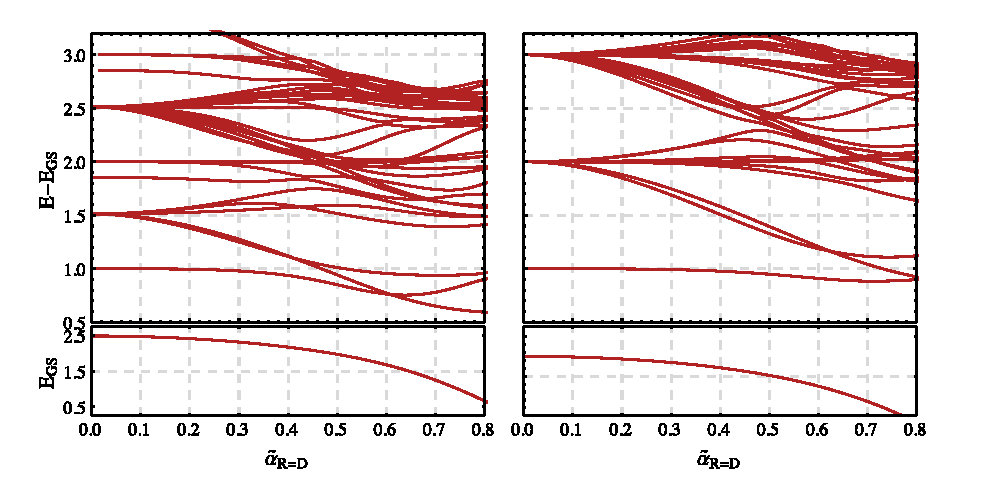
\includegraphics{SOC/Figures/RashbaDresselhausSpectrum}
\caption[Spectrum of states with even total angular momentum magnetic quantum number $J_z=0,2,\dots$ for the equal-weight Rashba-Dresselhaus coupling]{\label{fig:R=DExcitationSpectrum} 
Spectrum of states with even total angular momentum magnetic quantum number $J_z=0,2,\dots$ for the equal-weight Rashba-Dresselhaus SOC~\eqref{eq:R=D}. The left figure shows the energies with negative scattering length $\tilde{a}=-1$. The right figure shows the results in the unitary limit $|\tilde{a}|\rightarrow\infty$. The spectrum is symmetric about $\tilde{\alpha}_{R=D}=0$.} 
\end{figure}


\section{Conclusions}

In this chapter we have nonperturbatively calculated the spectrum of interacting two-particle systems with realistic spin-orbit couplings when the trapping potential cannot be ignored.  Matrix elements of a short-range pseudopotential and three types of spin-orbit coupling were determined analytically in a basis of the total angular momentum eigenstates of the interacting two-body problem without SOC. With the analytic matrix elements, exact diagonalization of the Hamiltonian within a finite basis was possible.

Our energy calculations were performed in a basis truncated in a consistent way by including all states below an energy cutoff. The resulting spectra show good convergence except in the case where the two-body interaction generates a small positive scattering length. In this regime coupling of the ground state to higher relative-coordinate excited states dominates and convergence in the cutoff parameter $E_{\text{max}}$ was numerically intractable. We are currently investigating alternative methods to deal with this issue. In the limit of weak SOC we have compared our results to the perturbative calculations of \cite{PhysRevA.89.033606} and found good agreement. We also observed that although the ground state does not couple strongly to center-of-mass excitations, their inclusion is crucial for the excited state spectrum.  The relatively weak center-of-mass coupling of the ground state, however, suggests that cold atoms with SOC can be used as a surrogate system to probe properties of two-body spin-orbit couplings, e.g., the parity-violating weak interaction in nuclear systems. 

We provided plots of a variety of spectra calculated with Weyl, Rashba, and equal weight Rashba-Dresselhaus couplings.  Although in this thesis we show spectra only within certain subspaces of conserved angular momentum quantum numbers, the approach presented is fully capable of generating results for all possible states. Larger SO-coupling constants are also accessible with larger basis sizes. The general method can easily be adapted to calculate energies for bosonic systems, or to new forms of SOC such as the recently proposed spin-orbital angular momentum coupling \cite{2014arXiv1411.1737S}.  

Using the eigenvectors of the truncated basis Hamiltonian, we also explored the effect of parity violation on the system. In particular we show how the SOC induces mixing of the positive- and negative-parity subspaces for the ground state. Without a two-body interaction, the ground state preferentially projects onto negative parity basis states even for modest SOC strength. The short-range interaction was seen to suppress this mixing, especially when the scattering length is positive.

A natural extension of this work is to consider three particles within a trap.  Because of the complex spectrum that is associated with three-body physics at the unitary limit (e.g., Efimov states, limit cycles, etc.), the spectrum under the influence of an external SOC is expected to be quite rich.  Couplings between the center-of-mass and relative motion due to the SOC present a potential challenge to traditional few-body techniques, such as the Faddeev equations, which work only within the relative coordinates.  However, in our two-body calculations we found that the coupling of the ground state to the c.m. motion is weak. If this is also true in the three-body case, then to a good approximation we can ignore the c.m. motion and utilize existing few-body techniques with little or no modification.  

%\chapter{\label{chap:SOC}Energy Spectra of Two Interacting Fermions with Spin-Orbit Coupling in a Harmonic Trap}

%\begin{abstract}
%We explore the two-body spectra of spin-$1/2$ fermions in isotropic harmonic traps with external spin-orbit potentials and short range two-body interactions. Using a truncated basis of total angular momentum eigenstates, nonperturbative results are presented for experimentally realistic forms of the spin-orbit coupling: a pure Rashba coupling, Rashba and Dresselhaus couplings in equal parts, and a Weyl-type coupling. The technique is easily adapted to bosonic systems and other forms of spin-orbit coupling.
%\end{abstract}

Cold atomic gases with parity-violating spin-orbit coupling (SOC) have recently been an area of intense interest because of the potential to simulate interesting physical systems with precisely tunable interactions \cite{nature11841}. In condensed-matter and atomic physics, spin-orbit couplings\footnote{In these fields, spin-orbit coupling conventionally refers to operators which couple spin with momentum, as opposed to the more restrictive use in nuclear and atomic physics where there term specifically refers to a parity-conserving $\vec{\ell}\cdot \vec{s}$ interaction.}\ are essential for many exotic systems such as topological insulators \cite{das2013engineering,PhysRevLett.105.255302}, the quantum spin Hall effect \cite{nature12185}, and spintronics \cite{RevModPhys.76.323}. The experimental setup which induces spin-orbit coupling is intimately related to simulation of synthetic gauge fields \cite{RevModPhys.83.1523,hamner2014dicke,Lin:2009zzb,Bermudez:2011db}. Because these couplings are parity violating, they potentially play similar roles within nuclear systems that undergo parity-violating transitions due to the nuclear weak force.  Atomic gases provide an excellent testing ground both to explore universal behavior of these real life systems and to create new types of spin-orbit coupling which are not yet known to exist (or have no solid-state analog) in other materials but are interesting in their own right. Further, these experiments can be performed in an environment with few or no defects and impurities.

Spin-orbit coupling was first realized in a Bose condensate of $^{87}$Rb \cite{nature09887} and extended shortly after to Fermi gases of $^{40}$K \cite{PhysRevLett.109.095301} and $^6$Li \cite{PhysRevLett.109.095302}. These spin-orbit interactions are `synthetic' in the sense that a subset of the hyperfine states stand in as virtual spin states. A particularly interesting consequence of this is the possibility of studying systems with synthetic spin-$1/2$ spin-orbit interactions but bosonic statistics \cite{PhysRevA.68.063612,nature09887}. From another point of view, the couplings are equivalent to applying external electromagnetic forces via synthetic gauge couplings on the physically uncharged particles in the gas \cite{Lin:2011,PhysRevLett.107.255301}. It has also been conjectured that these systems could be used to physically simulate lattice gauge theories \cite{Bermudez:2010da,Mazza:2011kf}.  Spin-orbit couplings in solid-state systems arise in two-dimensional (2D) systems (Rashba and Dresselhaus types, described in Sec.~\ref{sec:Hamiltonian}), but recently an experimental setup has been proposed that can simulate the Weyl-type SOC which is fundamentally three dimensional \cite{PhysRevLett.108.235301}.

Spin-orbit couplings are also of interest from the perspective of few-body physics where they arise in a variety of fields, e.g., the weak nuclear interactions governing proton-proton scattering \cite{Haxton:2013aca,deVries:2014vqa}. Because the spin-orbit coupling is long range, it can significantly modify both the threshold scattering behavior and the spectrum of two-body systems \cite{PhysRevA.86.042707}. For low-energy scattering, Duan \textit{et al.} \cite{PhysRevA.87.052708} showed analytically that parity-violating SOC leads to the the spontaneous emergence of handedness in outgoing states, a finding later confirmed in \cite{PhysRevA.91.022706}. Even in the presence of a repulsive two-body interaction, an arbitrarily weak SOC has been shown to bind dimers \cite{PhysRevB.83.094515}. For three-particle systems, a new type of universality is conjectured to occur for bound trimers with negative scattering length \cite{PhysRevLett.112.013201}. 

Few-atom systems undergoing SOC within trapping potentials have also been explored. For example, the spectrum of particles within a trap with an external SOC of the Weyl type (but no relative interaction) has been theoretically determined \cite{anderson2013}. The Rashba SOC with two-particle systems interacting via short-ranged interactions was investigated perturbatively in \cite{PhysRevA.89.033606}, where it was shown that the leading order corrections due to the SOC and short-range interaction are independent when the scattering length is equal for all channels.  In one dimension, the spectrum for this type of system has been calculated when the SOC consists of equal parts Rashba and Dresselhaus interactions \cite{guan2014energy}. Information learned from trapped systems augments that from scattering experiments while also being relevant to interesting phenomena in trapped many-body systems with SOC such as solitons \cite{DarkSolitons,PhysRevA.87.013614} or novel phase diagrams \cite{PhysRevLett.107.270401}.


In all these calculations, the emergent spectrum is rich and complex, offering new insights into few-body behavior.  Our objective is to provide some additional insight into two-body physics of Fermi gases with spin-orbit interactions in the presence of both three-dimensional trapping potentials and short-ranged two-body interactions, which are necessarily present in dilute cold-atom experiments. Our approach is to numerically diagonalize the Hamiltonian within a suitably truncated basis, and is thus nonperturbative in nature. Eigenstates of the interacting Hamiltonian without SOC are used for the basis. Section~\ref{sec:Hamiltonian} introduces the specific forms of spin-orbit coupling and two-body interactions which we consider. The general method is detailed in Sec.~\ref{sec:Weyl} for the simplest SOC.  In the remaining Secs.~\ref{sec:Rashba}-\ref{sec:R=D} we study the spectra of additional spin-orbit couplings in order of increasing computational complexity.

\section{\label{sec:Hamiltonian}Hamiltonian for Spin-orbit Couplings with Contact Interactions}

In this chapter we simply refer to our systems by their `spin' degrees of freedom and use the standard notation for spin quantum numbers. We consider three different types of spin-orbit coupling. The form of spin-orbit coupling realized in experiments is a linear combination of the Rashba \cite{0022-3719-17-33-015} and linear Dresselhaus \cite{PhysRev.100.580} types,
\begin{align}
V_{R}&\equiv\alpha_R (\sigma_x k_y-\sigma_y k_x) \label{eq:Rashba},\\
V_{D}&\equiv\alpha_D (\sigma_x k_y+\sigma_y k_x) \label{eq:Dresselhaus},
\end{align} 
which were originally recognized in two-dimensional solid-state systems. In a 2D system, these form a complete basis for spin-orbit couplings linear in momentum. Note that some references use the alternate definitions $V_R\propto  (\sigma_x k_x+\sigma_y k_y) $ and $V_D\propto  (\sigma_x k_x-\sigma_y k_y) $ which are equivalent up to a pseudospin rotation.  For solids, these parity-violating interactions are allowed only in the absence of inversion symmetries. Rashba-type SOC typically arises in the presence of applied electric fields or in 2D subspaces such as the surfaces of materials where the boundary breaks the symmetry. Dresselhaus couplings were first studied in the context of bulk inversion asymmetry, when the internal structure leads to gradients in the microscopic electric field. 

To date, experiments have produced only SOC potentials in which the Rashba and Dresselhaus terms appear with equal strength (also known as the ``persistent spin-helix symmetry point'' \cite{PhysRevLett.97.236601}), 
\begin{equation}
\label{eq:R=D}
V_{R=D}\equiv\alpha_{R=D}\sigma_x k_y.
\end{equation} 
After a pseudospin rotation, this potential can be seen as a unidirectional coupling of the pseudospin and momentum along a single axis. A proposal for tuning the ratio $\alpha_R/\alpha_D$ has been given in \cite{PhysRevA.84.025602}.  An experimental setup which gives the simple three-dimensional Weyl coupling,
\begin{equation}\label{eq:Weyl}
V_{W}\equiv\alpha_W \vec{k}\cdot\vec{\sigma},
\end{equation}
has also been proposed in \cite{PhysRevLett.108.235301} and \cite{PhysRevLett.111.125301}. 

In the following sections we calculate the spectra of two particles with a short-range two-body interaction, an isotropic harmonic trapping potential and spin-orbit coupling. The single particle Hamiltonian is 
\begin{equation}\label{eq:shortRangeInteraction}
H_1=\frac{\hbar^2 k^2}{2m}+\frac{1}{2}m\omega^2 r^2 + V_{\text{SO}}.
\end{equation}
For the spin-orbit term $V_{\text{SO}}$, we consider equal Rashba and Dresselhaus~\eqref{eq:R=D}, pure Rashba~\eqref{eq:Rashba}, and Weyl~\eqref{eq:Weyl} spin-orbit couplings  because these are generally considered to be experimentally feasible.

We assume that the range of interaction between particles is small compared to the size of the oscillator well.  The relative interaction between the particles can then be approximated as a regulated $s$-wave contact interaction, which in momentum space (as a function of relative momentum) is given by
\begin{equation}
\frac{4\pi \hbar^2}{m}a(\Lambda)\ .
\end{equation}
Here the argument $\Lambda$ refers to some cutoff scale and $a(\Lambda)$ is some function of the cutoff and physical scattering length $a_{\text{phys}}$.  The exact form of this function depends on the type of regulator used and is not relevant for this work; the only constraint is that $a(\Lambda)$ reproduce the physical scattering length given by the scattering $T$ matrix at threshold, $T(E=0)=4\pi\hbar^2 a_{\text{phys}}/m$ \cite{taylor2000}. In the limit $\Lambda\rightarrow \infty$ the spectrum of two particles in an oscillator well (without external spin-orbit interaction) was solved by Busch \textit{et al.} \cite{Busch} using the method of pseudopotentials.  In Ref.  \cite{Luu:2006xv} the solution for general $\Lambda$ was given using a Gaussian regulator, which in the limit $\Lambda\rightarrow\infty$ recovered the Busch \textit{et al.} solution.  For our work below we use the eigenstates and eigenvalues of this two-particle system given in Ref. \cite{Busch}.

\section{\label{sec:Weyl}Weyl Coupling}
We tackle the Weyl form first because of its mathematical and numerical simplicity. In the absence of the two-body interaction, this problem was treated in Ref. \cite{anderson2013}. Our approach is to determine the matrix elements of the SOC in an appropriate basis. The eigenvalue is then solved numerically at the desired precision by choosing an appropriately large truncated basis of harmonic oscillator (HO) eigenstates.

As usual, the two-body problem is best approached in the dimensionless Jacobi coordinates
\begin{equation}
R=\frac{r_1+r_2}{\sqrt{2}b}, \qquad r=\frac{r_1-r_2}{\sqrt{2}b}
\end{equation}
and the corresponding conjugate momenta $q,Q$ representing the relative and total momenta. For an isotropic harmonic oscillator, distances can be expressed in terms of the ground-state length scale $b=\sqrt{\hbar/m\omega}$ and energies will be similarly measured in units of $E_0=\hbar\omega$. We also define the spin operators
\begin{equation}
\vec{\sigma}\equiv\vec{\sigma}_1-\vec{\sigma}_2, \qquad \vec{\Sigma}\equiv\vec{\sigma}_1+\vec{\sigma}_2.
\end{equation}

With these definitions, the two-body Hamiltonian can be nondimensionalized and separated into relative and center-of-mass (c.m.) parts,
\begin{equation}\label{eq:WeylHamiltonian}
\frac{1}{\hbar\omega}H=\left(h_{0,\text{rel}}+\frac{\tilde{\alpha}_W}{\sqrt{2}} \vec{q}\cdot\vec{\sigma} + \sqrt{2}\pi \tilde{a}(\Lambda) \delta^{(3)}(r)\right)+\left(h_{0,\text{c.m.}}+\frac{\tilde{\alpha}_W}{\sqrt{2}} \vec{Q}\cdot\vec{\Sigma} \right),
\end{equation}
where $h_{0,\text{rel}}=r^2/2$ and $h_{0,\text{c.m.}}=R^2/2$. Notably, the spin-orbit coupling appears in both terms.  The tilde over the coupling constants indicates that they are dimensionless, related to the original coupling constants by e.g., $\tilde{\alpha}_W=\alpha_W/(\hbar\omega b)$. Similarly the scattering length is made dimensionless by dividing out the oscillator length, $\tilde{a}=a/b$. Throughout the remainder of this chapter we will refer to dimensionless eigenvalues of $H/\hbar\omega$ as the energies of the system.

%We point out that the relative-coordinate spin-orbit term in Eq.~\eqref{eq:WeylHamiltonian} is exactly of the form that appears in weak-interaction parity-violating proton-proton scattering \cite{Haxton:2013aca,deVries:2014vqa}.  Aside from Coulomb contributions, the $^1S_0$ channel of proton-proton scattering has a scattering length that is an order of magnitude larger than its effective range.  The parity-conserving part of the nuclear potential could therefore be represented by the contact interaction in Eq.~\eqref{eq:WeylHamiltonian}.  The CM spin-orbit term (i.e. the last term in Eq.~\eqref{eq:WeylHamiltonian}) spoils this analogy. However, we will show later that the effect of this term on the ground state is negligible. 

\begin{figure}
\centering
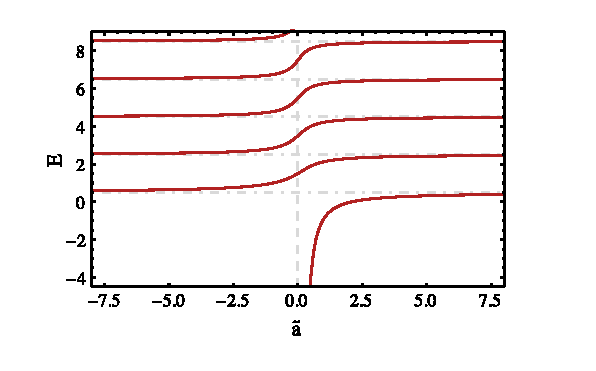
\includegraphics[scale=1.2]{SOC/Figures/BuschSpectrum}
\caption[Spectrum of the two-body contact interaction Hamiltonian as a function of $\tilde a$]{\label{fig:BuschSpectrum} Spectrum of the two-body contact interaction Hamiltonian as a function of $\tilde a$. The horizontal lines indicate the dimensionless energy eigenvalues in the unitary limit $|\tilde{a}|\rightarrow\infty$.} 
\end{figure}

Eigenstates of two particles with a short-range interaction in a harmonic oscillator trapping potential form a convenient basis for these calculations. These basis functions were first derived in \cite{Busch} for the isotropic case considered here, and the more general case of an anisotropic trap has been explored in \cite{PhysRevA.74.022712}. The dependence of the energy spectrum on the scattering length $a$ is shown in Fig.~\ref{fig:BuschSpectrum} for reference. Qualitatively, the effect of the short-range interaction is to shift the harmonic oscillator energies by $\pm \hbar\omega$ as the scattering length goes to $\pm \infty$. For positive scattering length, there is also an additional negative-energy dimer state.

We choose the particular coupling scheme of angular momentum eigenstates,
\begin{equation}\label{eq:basisStates}
\ket{n(ls)j;NL;(jL)J},
\end{equation}
which simplify the matrix elements for the relative-coordinate operators. Here $n$ and $l$ refer to the principal and orbital angular-momentum quantum numbers of the two-particle system in the relative coordinates. $N$ and $L$ refer to the analogous numbers in the center-of-mass frame. The total spin of the two spin-$1/2$ particles is denoted by $s = s_1 + s_2$ and may be either 0 or 1. First $s$ and $l$ to make angular momentum $j$, which is then recoupled with the c.m. angular momentum $L$ to make the state's total angular momentum $J$. Because all terms in the Hamiltonian~\eqref{eq:WeylHamiltonian} are scalars, the interaction is independent of $J_z$ and so we omit this quantum number for clarity. Due to Pauli exclusion, $l + s$ must be even to enforce antisymmetry under exchange of the particles.

For $l\neq0$ the states~\eqref{eq:basisStates} are identical to the well known harmonic oscillator, with $n$ and $l$ ($N$ and $L$) indicating the relative (center-of-mass) HO quantum numbers. We use the convention that $n,N=0,1,2,\dots$, and therefore $E=2n+l+2N+L+3$. The short range interaction~\eqref{eq:shortRangeInteraction} modifies the $l=0$ states and their spectrum. The principal relative quantum number $n$ for these states is obtained by solving the transcendental equation
\begin{equation}\label{eq:eigenvalueEqn}
\sqrt{2}\frac{\Gamma(-n)}{\Gamma(-n-1/2)}=\frac{1}{\tilde{a}}
\end{equation}
and is no longer integer valued. For the relative-coordinate part of the $l=0$ wave function,
\begin{align}
\phi(r)&=\frac{1}{2\pi^{3/2}}A(n)\Gamma(-n)U(-n,3/2,r^2)e^{-r^2/2}, \label{eq:BuschWF}\\
A(n)&=\left(\frac{\Gamma(-n)[\psi_0(-n)-\psi_0(-n-1/2)]}{8 \pi^2 \Gamma(-n-1/2)}\right)^{-1/2},
\end{align}
where $U(a,b,x)$ is Kummer's confluent hypergeometric function and $\psi_0(x)=\Gamma'(x)/\Gamma(x)$ is the digamma function. A derivation of the normalization factor $A(n)$ is given in the Appendix.

Standard angular momentum algebra can be used to determine the matrix elements of the two spin-orbit coupling terms; we follow the conventions of \cite{Edmonds}. For Weyl SOC of two spin-$1/2$ fermions, the matrix elements of the coupling in the relative momentum are
\begin{equation}\label{eq:WeylRel}\begin{split}
\bra{n'(l's')j';N'L';(j'L')J'}\vec{q}&\cdot\vec{\sigma} \ket{n(ls)j;NL;(jL)J}  \\
=&\delta_{N,N'}\delta_{L,L'}\delta_{j,j'}\delta_{J,J'}(-1)^{l+s'+j}\frac{3}{\sqrt{2}}\sixj{j}{s'}{l'}{1}{l}{s} (s'-s)\braket{n'l' || q || n l}.
\end{split}
\end{equation}
To preserve anti-symmetry of the two-particle system, the relative momentum term in the Weyl SOC must couple states with relative angular momentum $l$ to $l\pm 1$, leaving $l+s$ even but changing the parity.

For basis states with both $l,l'\neq0$, reduced matrix elements of the momentum operator are calculated between pure harmonic oscillator states,
% Could do away with some constants in favor of the 3-j coefficient
\begin{align}
\braket{n'l' || q || n l}=&(-1)^{l'}(-1)^{\frac{l+l'+1}{2}}\sqrt{\frac{2(2l+1)(2l'+1)}{(l+l'+1)}}\braket{n'l'0| (-i \nabla_0) | n l 0} \\
\begin{split} =& i(-1)^{l}\sqrt{\frac{l+l'+1}{2}}\sqrt{n!n'!\Gamma(n+l+3/2)\Gamma(n'+l'+3/2)} \\ 
&\times\sum_{m,m'=0}^{n,n'} \left\{
     \begin{array}{lr}
       \frac{(-1)^{m+m'}\left[2m\Gamma\left(m+m'+1+\frac{l+l'}{2}\right)-\Gamma\left(m+m'+1+\frac{l+l'}{2}\right)\right]}{m!m'!(n-m)!(n'-m')!\Gamma(m+l+3/2)\Gamma(m'+l'+3/2)} & \text{if}\: l'=l-1 \\
        \frac{(-1)^{m+m'+1}\left[(2m+2l+1)\Gamma\left(m+m'+1+\frac{l+l'}{2}\right)-\Gamma\left(m+m'+1+\frac{l+l'}{2}\right)\right]}{m!m'!(n-m)!(n'-m')!\Gamma(m+l+3/2)\Gamma(m'+l'+3/2)} & \text{if}\: l'=l+1 \\
       0 & \text{otherwise}
     \end{array}
   \right.
   \end{split}
\end{align}
If $l=1$ and $l'=0$ or vice versa, reduced matrix elements between one modified wave function of the form~\eqref{eq:BuschWF} and one pure harmonic oscillator state are needed. These are given by
\begin{align}
\braket{n l=0 || q || n' l'=1}=-i A(n) \sqrt{\frac{\Gamma(n'+5/2)}{2\pi^3 n'!}}\frac{2n-2n'-1}{2(n'-n)(1+n'-n)}
\end{align}
and its Hermitian conjugate.

Our choice of basis makes the relative matrix elements~\eqref{eq:WeylRel} simple at the cost of complicating the center-of-mass term. We take the approach of expanding the states~\eqref{eq:basisStates} in the alternate coupling scheme,
\begin{equation}\label{eq:basisStates2}
\ket{n(ls)j;NL;(jL)J}=(-1)^{l+s+L+J}\sqrt{2j+1}\sum_{\mathcal{J}}\sqrt{2\mathcal{J}+1}\sixj{l}{s}{j}{L}{J}{\mathcal{J}}\ket{nl;N(Ls)\mathcal{J};(l\mathcal{J})J}.
\end{equation}
Using this notation, the matrix elements can be written
\begin{equation}\begin{split}
\bra{n'(l's')j';N'L';(j'L')J'}&\vec{Q}\cdot\vec{\Sigma} \ket{n(ls)j;NL;(jL)J} = \delta_{n,n'}\delta_{l,l'}\delta_{J,J'}\delta_{s,1}\delta_{s1,1}   6 (-1)^{L} \\
&\hspace{-2cm}\times\braket{N'L'|| \vec{Q} || NL} \sum_{\mathcal{J}}(-1)^\mathcal{J} (2\mathcal{J}+1)\sixj{l}{1}{j'}{L'}{J}{\mathcal{J}}\sixj{l}{1}{j}{L}{J}{\mathcal{J}}\sixj{\mathcal{J}}{1}{L'}{1}{L}{1}.
\end{split}
\end{equation}
Again, the reduced matrix element of the center-of-mass momentum changes the parity by connecting states with $\Delta L=\pm1$. Matrix elements are nonzero only for $\Delta s=0$ because the antisymmetry of the spatial wave function depends only on $l$, which does not change. We also note that the c.m. term does not affect states with singlet spin wave functions ($s=0$).


\begin{figure}
\centering
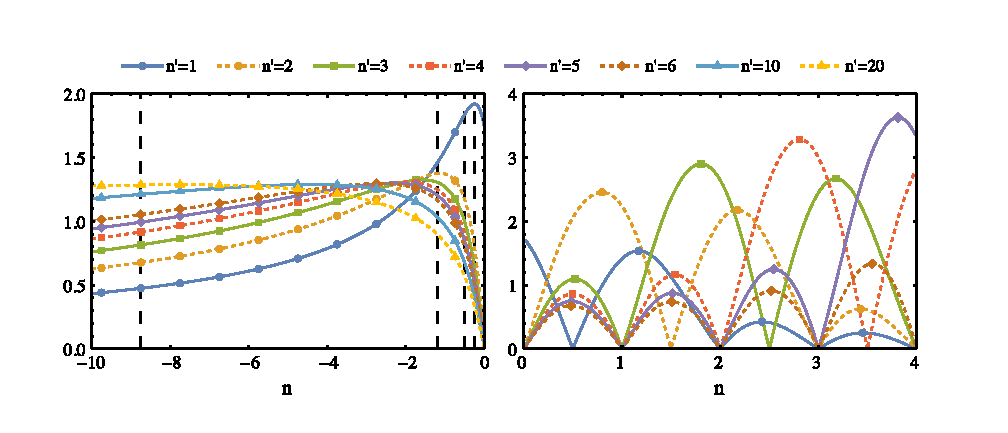
\includegraphics{SOC/Figures/MatrixElts}
\caption[Coupling of ground state to $l=1$ states for the Weyl spin-orbit Hamiltonian]{\label{fig:matrixElts}Absolute value of the matrix elements $|\bra{n'(11)0;00;(00)0}\vec{\sigma}\cdot\vec{q}\ket{n(00)0;00;(00)0}|$ between the ground state and $l=1$ excited states. The horizontal axis is the principal quantum number of the ground state obtained by solving~\eqref{eq:eigenvalueEqn}. From left to right, the vertical lines on the negative axis indicate the values obtained for $\tilde{a}=1/4$, $\tilde{a}=1$, $\tilde{a}=\pm\infty$, and $\tilde{a}=-1$, respectively.} 
\end{figure}

Using these matrix elements, we calculated the spectrum of the two interacting particles with Weyl spin-orbit coupling. Our calculations are performed by numerically diagonalizing in a truncated basis of the harmonic oscillator states~\eqref{eq:basisStates}, where a cutoff $2N+L+\nobreak 2n+\nobreak l+ \nobreak3\leq\nobreak E_{\text{max}}$ is set high enough that the eigenvalues of the matrix have converged to the desired accuracy.  

\begin{figure}
\centering
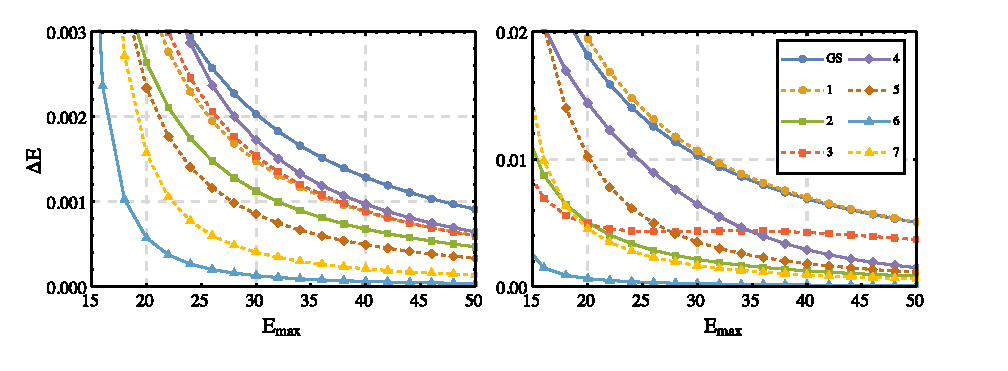
\includegraphics{SOC/Figures/WeylConvergence}
\caption[Convergence of the energy eigenvalues for the Weyl spin-orbit coupling]{\label{fig:WeylConvergence}  A convergence plot giving the change in energy eigenvalue, $\Delta E$, for the lowest eight energy levels when a shell is added as a function of $E_{\text{max}}$.  The left figure shows convergence for $\tilde{a}=-1$ and $\tilde{\alpha}_W=0.5$. In the right panel  we show $\tilde{a}=1$ and $\tilde{\alpha}_W=0.5$, demonstrating that convergence of the states with large negative $n$ is poor.} 
\end{figure}

This approach converges well only when the ground-state energy is not too low. In particular, for $a$ positive but very small the principal quantum number of the ground state is increasing from negative infinity as seen in Fig.~\ref{fig:BuschSpectrum}. From Fig.~\ref{fig:matrixElts}, we can see that as $n$ becomes more negative, the principal quantum number of the dominant matrix element is also increasing. Because convergence of any energy level requires a cutoff much larger than the energy of the most strongly coupled states, a sufficiently high $E_{\text{max}}$ to ensure an accurate ground-state energy becomes infeasible for small positive $a$. For excited states, $n$ is always positive and matrix elements with similar $n$ always dominate. The strength of the matrix elements follows a similar qualitative behavior for the spin-orbit couplings treated in the following sections where the same issues recur. 

\begin{figure}
\centering
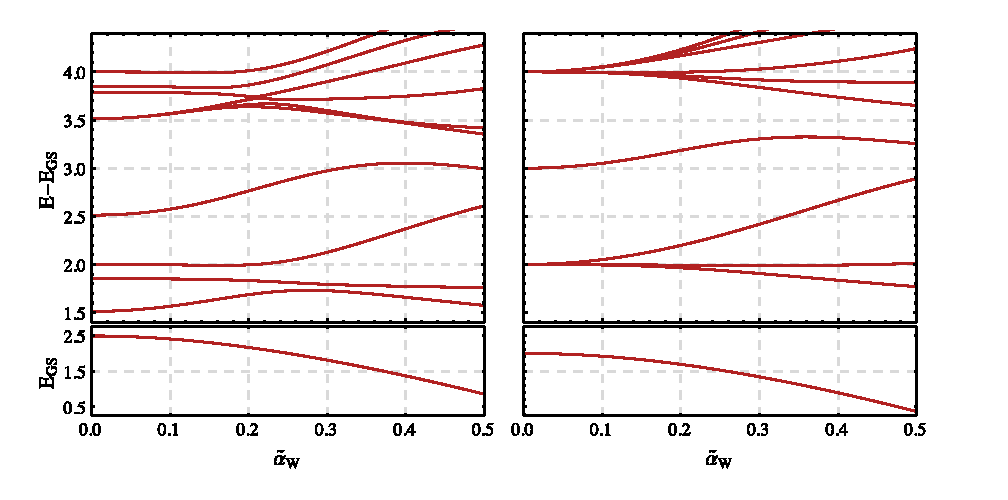
\includegraphics{SOC/Figures/WeylSpectrum}
\caption[Spectrum of states with $J=0$ for Weyl spin-orbit coupling]{\label{fig:WeylSpectrum}  Spectrum of states with total angular momentum $J=0$ for the dimensionless Hamiltonian~\eqref{eq:WeylHamiltonian}. The bottom left figure shows the ground-state energy for $\tilde{a}=-1$ as a function of $\tilde{\alpha}_W$; above are the first few excitation energies. The right figure shows the results in the unitary limit of the two-body interaction, $|\tilde{a}|\rightarrow\infty$. The spectrum is symmetric about $\tilde{\alpha}_W=0$.} 
\end{figure}

As a result, convergence of the ground state is actually slower than that for nearby excited states. Furthermore, our approach gives the fastest convergence when $a$ is not small and positive. We compare the rate of convergence of the $\tilde{a}=-1$ and $\tilde{a}=1$ spectra in Fig.~\ref{fig:WeylConvergence} to demonstrate the dependence of convergence on the matrix truncation. The actual energy spectrum is shown in Fig.~\ref{fig:WeylSpectrum}. 

\begin{figure}
\centering
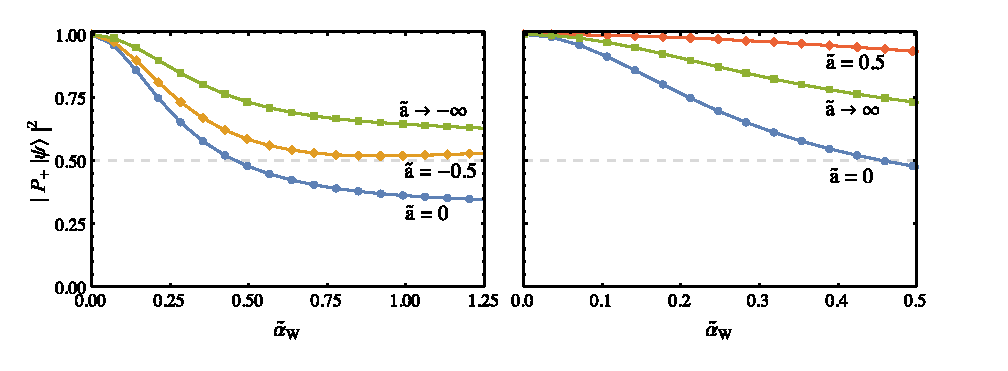
\includegraphics{SOC/Figures/Projections}
\caption[Parity projection of the Weyl spin-orbit coupling ground state]{\label{fig:Projections} For different values of the two-body coupling strength $\tilde{a}$, we show the magnitude of the ground state projected onto even parity basis states as a function of the SOC strength. This is given by $\big|  P_+\ket{\psi_{\text{GS}}}\big|^2=\big| (1- P_-)\ket{\psi_{\text{GS}}}\big|^2$, where $P_+$ ($P_-$) is the projection operator onto the positive\nobreak- (negative\nobreak-) parity basis states. The left figure shows negative $\tilde{a}$, while the right shows positive $\tilde{a}$. Note that the limits $\tilde{a}\rightarrow\pm\infty$ are physically identical.}
\end{figure}

One consequence of parity violation in this system is that the eigenstates are mixtures of the even- and odd-parity basis states described by Eq.~\eqref{eq:basisStates}. In Fig.~\ref{fig:Projections} we visualize how these subspaces are mixed in the ground state as the SOC strength increases. For the noninteracting system, $\tilde{a}=0$, more than half of the ground state projects onto negative-parity states even at fairly small values of $\tilde{\alpha}_W$. However, we see that the short-range interaction reduces this effect. With negative $\tilde{a}$, the mixing of the negative-parity states is suppressed as the strength of the two-body interaction increases. When $\tilde{a}$ is positive the effect is more striking. Mixing with negative-parity states is most strongly suppressed for small positive values of $\tilde{a}$, while the projection onto these states increases for larger positive values. The admixture is qualitatively the same when considering other forms of SOC as described in the following sections.

\section{\label{sec:Rashba}The Pure Rashba Coupling}

In order to find the matrix elements of the pure Rashba coupling given in~\eqref{eq:Rashba}, we first note that it can be written as a spherical tensor
\begin{equation}
V_{R}=i\sqrt{2}\:\alpha_R \left[ k \otimes \sigma \right]_{10}.
\end{equation}
We therefore have the two-body Hamiltonian
\begin{equation}\label{eq:RashbaHamiltonian}
\frac{1}{\hbar\omega}H=\left(h_{0,\text{rel}}+i \tilde{\alpha}_R  \left[ \vec{q} \otimes \vec{\sigma} \right]_{10} + \sqrt{2}\pi \tilde{a}(\Lambda) \delta^{(3)}(r)\right)+\left(h_{0,\text{c.m.}}+i \tilde{\alpha}_R [ \vec{Q}\otimes \vec{\Sigma} ]_{10} \right).
\end{equation}

Because the spin-orbit coupling is now a $k=1$ tensor rather than a scalar operator, the total angular momentum $J$ is no longer conserved. Additionally, the matrix elements now depend on the quantum number $J_z$ (which is conserved). For the relative-coordinate part of the SOC, some algebra gives
\begin{equation}\begin{split}
&\bra{n'(l's')j';N'L';(j'L')J'J'_z}  [ \vec{q} \otimes \vec{\sigma} ]_{10}  \ket{n(ls)j;NL;(jL)JJ_z} = \\
&\hspace{1.5cm} 6 i (-1)^{J+J'-J'_z+j'+L+1}\delta_{N,N'}\delta_{L,L'}\delta_{J_z,J'_z} \sqrt{(2J+1)(2J'+1)(2j+1)(2j'+1)} \\
 &\hspace{2.7cm} \times \threej{J'}{1}{J}{-J_z}{0}{J_z} \sixj{j'}{J'}{L}{J}{j}{1}
 \renewcommand{\arraystretch}{0.9}
 \ninej{\hphantom{l}l'\hphantom{l}}{\hphantom{l}l\hphantom{l}}{\hphantom{l}1\hphantom{l}}{s'}{s}{1}{j'}{j}{1} (s'-s) \braket{n'l' || q || n l}.
\end{split}
\end{equation}
For the center-of-mass part of the Hamiltonian we again expand the basis states in the alternate coupling scheme~\eqref{eq:basisStates2} to obtain the matrix elements
\begin{equation}\begin{split}
&\bra{n'(l's')j';N'L';(j'L')J'J'_z} [ \vec{Q} \otimes \vec{\Sigma} ]_{10}  \ket{n(ls)j;NL;(jL)JJ_z} = \delta_{n,n'}\delta_{l,l'}\delta_{J_z,J'_z}\delta_{s,1}\delta_{s',1} \\
 &\quad\times 6 i \sqrt{2}(-1)^{J+J'-J'_z+l} \sqrt{(2J+1)(2J'+1)(2j+1)(2j'+1)} \threej{J'}{1}{J}{-J_z}{0}{J_z}  \braket{N' L' || Q || N L} \\ 
 &\quad\times\sum_{\mathcal{J},\mathcal{J}'} (-1)^\mathcal{J}(2\mathcal{J}+1)(2\mathcal{J}'+1)\sixj{l}{1}{j'}{L'}{J'}{\mathcal{J}'}\sixj{l}{1}{j}{L}{J}{\mathcal{J}}\sixj{\mathcal{J}'}{J'}{l}{J}{\mathcal{J}}{1}
 \renewcommand{\arraystretch}{0.9}
 \ninej{\hphantom{l}L'\hphantom{l}}{\hphantom{l}L\hphantom{l}}{\hphantom{l}1\hphantom{l}}{1}{1}{1}{\mathcal{J}'}{\mathcal{J}}{1} .
\end{split}
\end{equation}

\begin{figure}
\centering
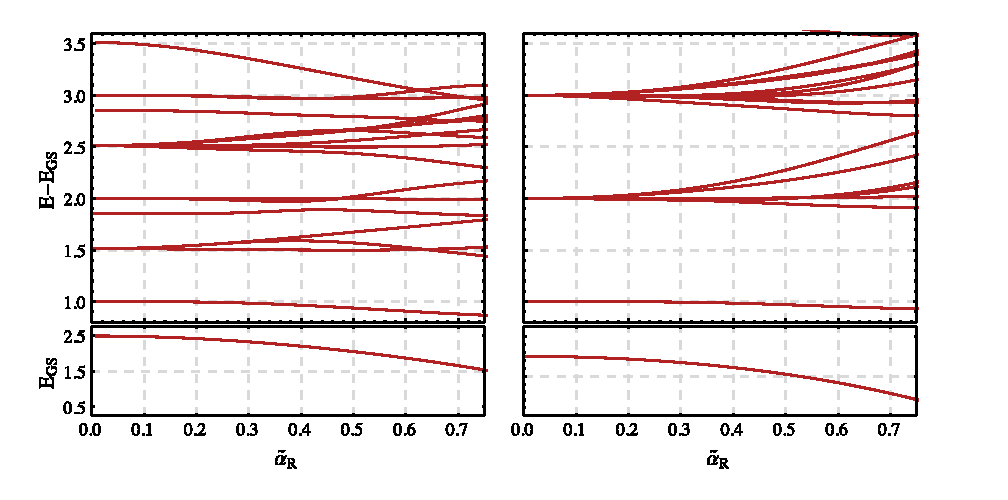
\includegraphics{SOC/Figures/RashbaSpectrum}
\caption[Spectrum of the Rashba spin-orbit coupling for $J_z=0$]{\label{fig:RashbaSpectrum}  Spectrum of states with total angular momentum quantum number $J_z=0$ for the Hamiltonian~\eqref{eq:RashbaHamiltonian}. The left figure shows the energies with negative scattering length $\tilde{a}=-1$. The right figure shows the results in the unitary limit $|\tilde{a}|\rightarrow\infty$. The spectrum is symmetric about $\tilde{\alpha}_R=0$.} 
\end{figure}


Our results for the Rashba SOC are shown in Fig.~\ref{fig:RashbaSpectrum}. Because the Rashba spin-orbit coupling is a vector operator, states of all possible $J$ must be included in any calculation and the size of the basis scales much more quickly with $E_{\text{max}}$. These spectra were computed with an $E_{\text{max}}$ of $24\hbar\omega$, for which there are approximately $36\,000$ basis states. All displayed eigenvalues of the Hamiltonian shift by less than $10^{-2}\hbar\omega$ if an additional shell of states is included.

\begin{figure}
\centering
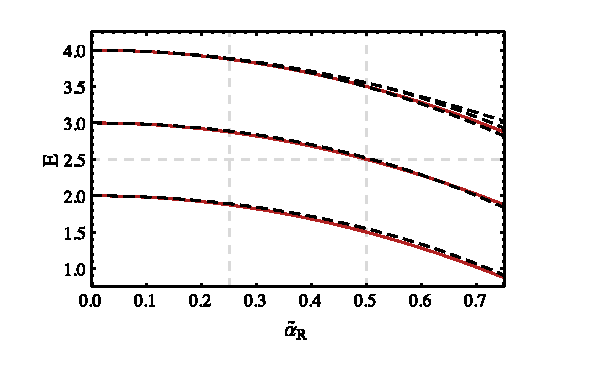
\includegraphics[scale=1.2]{SOC/Figures/PerturbativeComparison}
\caption[Comparison of the Rashba spectrum with perturbative predictions]{\label{fig:ComparisonSpectrum}Comparison of selected spectral lines (dashed black) with the perturbative predictions from \cite{PhysRevA.89.033606} (solid red) when $\tilde{a}=\infty$. }
\end{figure}

\begin{figure}
\centering
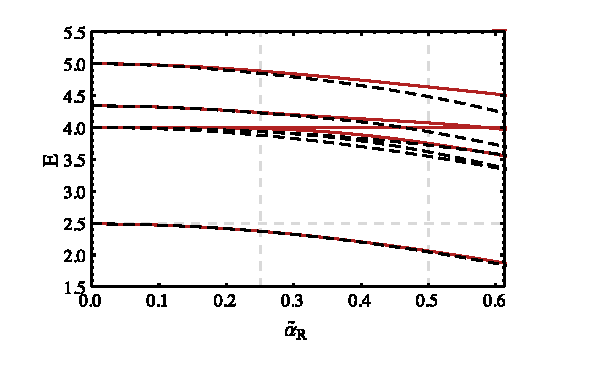
\includegraphics[scale=1.2]{SOC/Figures/ComparisonNoCM}
\caption[Effect of neglecting center of mass excitations for Rashba spin-orbit coupling]{\label{fig:ComparisonSpectrum2}  A comparison of the energy levels with (dashed black) and without (solid red) the inclusion of excitations in the c.m. coordinate for $\tilde{a}=-1$. The approximation of ignoring c.m. excitations provides very accurate results for the ground state, but not for excited states.} 
\end{figure}


This interaction was also studied perturbatively for small $\alpha_R$ in \cite{PhysRevA.89.033606}, including the possibility of a spin-dependent two-body interaction, under the assumption that center-of-mass excitations are unimportant. For the specific case of identical fermions with spin-independent scattering length considered here, they found that the first correction to the energies occurs at order $\alpha_R^2$ and is independent of the scattering length $a$. We compare their perturbative predictions, which are derived from the non-degenerate theory, with our numerical results in Fig.~\ref{fig:ComparisonSpectrum}. 

By setting all matrix elements with $N,L>0$ in the bra or ket to zero, we also explored the approximation of ignoring center-of-mass excitations. Fig.~\ref{fig:ComparisonSpectrum2} shows that this is very accurate for the ground state, but less accurate for excited states. Suppression of the c.m. coordinate has a similar effect for the SOCs considered in Secs.~\ref{sec:Weyl} and~\ref{sec:R=D}. We also note that in the case of small positive $a$, the landscape of low-lying excited states is dominated by center-of-mass excitations. When $a\rightarrow0^+$ in the absence of spin-orbit coupling, there are an infinite number of states with nonzero c.m. quantum numbers whose energies lie between the ground state and the first relative-coordinate excitation.


\section{\label{sec:R=D}Equal-Weight Rashba-Dresselhaus Spin-Orbit Coupling}

Experiments have thus far realized only the effective Hamiltonian with equal strength Rashba and Dresselhaus couplings in the form~\eqref{eq:R=D}. Energy levels of the two-body system in the one-dimensional equivalent of this Hamiltonian with the additional magnetic field couplings present in experimental realizations have been calculated in \cite{guan2014energy}. Here we treat the problem in three dimensions.

This is also the most computationally difficult of the three cases. When decomposed into spherical tensors, the interaction~\eqref{eq:Dresselhaus} becomes
\begin{equation}
V_D=i\,\alpha_D \left( \left[ k \otimes \sigma \right]_{2,-2}- \left[ k \otimes \sigma \right]_{2,2}\right),
\end{equation}
and the two-particle Hamiltonian in the presence of equal strength Rashba and Dresselhaus SOC is given by~\eqref{eq:RashbaHamiltonian} with $\alpha_R\rightarrow \alpha_{R=D}$ plus the additional spin-orbit terms
\begin{equation}\label{eq:DresselhausHamiltonian}
\Delta H= \frac{i \tilde{\alpha}_{R=D}}{\sqrt{2}}\left(  \left[ \vec{q} \otimes \vec{\sigma} \right]_{2,-2} -  \left[ \vec{q} \otimes \vec{\sigma} \right]_{2,2} +[ \vec{Q} \otimes \vec{\Sigma} ]_{2,-2} -  [ \vec{Q} \otimes \vec{\Sigma} ]_{2,2} \right).
\end{equation} 
Yet again the number of basis states with nonzero matrix elements has increased; no angular momentum quantum numbers are conserved. The only remaining selection rule will be that the interaction does not change the total magnetic quantum number $J_z$ between even and odd. 

Using the same approach as in the previous sections, the matrix elements of the relative Dresselhaus term are
\begin{equation}\begin{split}
&\bra{n'(l's')j';N'L';(j'L')J'J'_z} \frac{i \tilde{\alpha}_{R=D}}{\sqrt{2}}\left(  \left[ \vec{q} \otimes \vec{\sigma} \right]_{2,-2} -  \left[ \vec{q} \otimes \vec{\sigma} \right]_{2,2} \right)  \ket{n(ls)j;NL;(jL)JJ_z}  \\
 &\quad\hphantom{\times}= i \sqrt{30}(-1)^{J+J'-J'_z+j'+L}\delta_{N,N'}\delta_{L,L'} \sqrt{(2J+1)(2J'+1)(2j+1)(2j'+1)}  \braket{n'l' || q || n l}\\
 &\hspace{1cm}\quad \times(s'-s) \left[\threej{J'}{2}{J}{-J'_z}{-2}{J_z}-\threej{J'}{2}{J}{-J'_z}{2}{J_z}\right] \sixj{j'}{J'}{L}{J}{j}{2}
 \renewcommand{\arraystretch}{0.9} \ninej{\hphantom{l}l'\hphantom{l}}{\hphantom{l}l\hphantom{l}}{\hphantom{l}1\hphantom{l}}{s'}{s}{1}{j'}{j}{2},
\end{split}
\end{equation}
while the center-of-mass part is 

\begin{equation}\begin{split}
&\bra{n'(l's')j';N'L';(j'L')J'J'_z}  \frac{i \tilde{\alpha}_{R=D}}{\sqrt{2}}\left(  \left[ \vec{Q} \otimes \vec{\Sigma} \right]_{2,-2} -  \left[ \vec{Q} \otimes \vec{\Sigma} \right]_{2,2} \right)  \ket{n(ls)j;NL;(jL)JJ_z}   \\
&\quad=2 i \sqrt{15}(-1)^{J+J'-J'_z+l+1}\delta_{n,n'}\delta_{l,l'}\delta_{s,1}\delta_{s',1}  \\
 &\quad\hphantom{=}\times \sqrt{(2J+1)(2J'+1)(2j+1)(2j'+1)} \left[\threej{J'}{2}{J}{-J'_z}{-2}{J_z}-\threej{J'}{2}{J}{-J'_z}{2}{J_z}\right] \braket{N' L' || Q || N L} \\ 
 &\quad\hphantom{=}\times\sum_{\mathcal{J},\mathcal{J}'} (-1)^\mathcal{J}(2\mathcal{J}+1)(2\mathcal{J}'+1)\sixj{l}{1}{j'}{L'}{J'}{\mathcal{J}'}\sixj{l}{1}{j}{L}{J}{\mathcal{J}}\sixj{\mathcal{J}'}{J'}{l}{J}{\mathcal{J}}{2}
 \renewcommand{\arraystretch}{0.9}
 \ninej{\hphantom{l}L'\hphantom{l}}{\hphantom{l}L\hphantom{l}}{\hphantom{l}1\hphantom{l}}{1}{1}{1}{\mathcal{J}'}{\mathcal{J}}{2} .
\end{split}
\end{equation}

The richly structured excitation spectrum of low-lying states is shown in Fig.~\ref{fig:R=DExcitationSpectrum} for a cutoff of $E_{\text{max}}=17$. All displayed energies shift by less than .$02\hbar\omega$ when the final shell is added, giving a slightly faster convergence than in the pure Rashba case.

\begin{figure}
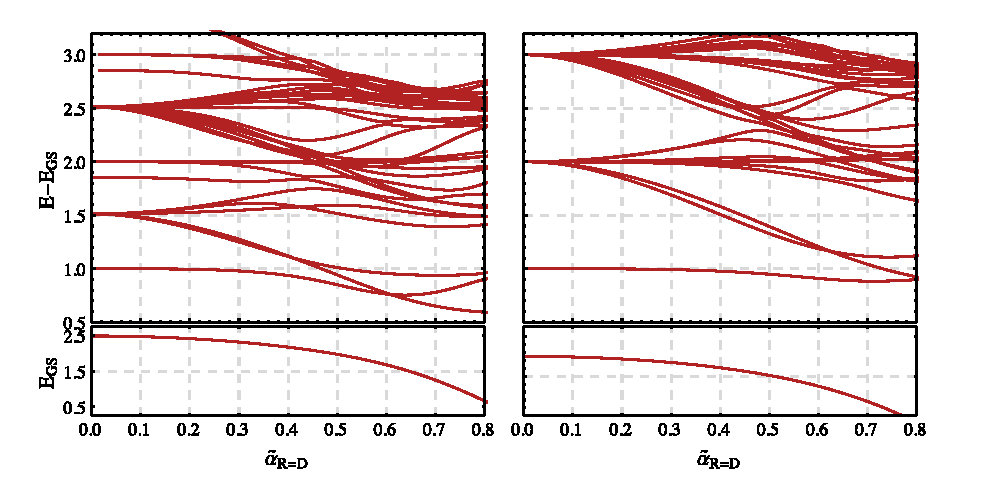
\includegraphics{SOC/Figures/RashbaDresselhausSpectrum}
\caption[Spectrum of states with even total angular momentum magnetic quantum number $J_z=0,2,\dots$ for the equal-weight Rashba-Dresselhaus coupling]{\label{fig:R=DExcitationSpectrum} 
Spectrum of states with even total angular momentum magnetic quantum number $J_z=0,2,\dots$ for the equal-weight Rashba-Dresselhaus SOC~\eqref{eq:R=D}. The left figure shows the energies with negative scattering length $\tilde{a}=-1$. The right figure shows the results in the unitary limit $|\tilde{a}|\rightarrow\infty$. The spectrum is symmetric about $\tilde{\alpha}_{R=D}=0$.} 
\end{figure}


\section{Conclusions}

In this chapter we have nonperturbatively calculated the spectrum of interacting two-particle systems with realistic spin-orbit couplings when the trapping potential cannot be ignored.  Matrix elements of a short-range pseudopotential and three types of spin-orbit coupling were determined analytically in a basis of the total angular momentum eigenstates of the interacting two-body problem without SOC. With the analytic matrix elements, exact diagonalization of the Hamiltonian within a finite basis was possible.

Our energy calculations were performed in a basis truncated in a consistent way by including all states below an energy cutoff. The resulting spectra show good convergence except in the case where the two-body interaction generates a small positive scattering length. In this regime coupling of the ground state to higher relative-coordinate excited states dominates and convergence in the cutoff parameter $E_{\text{max}}$ was numerically intractable. We are currently investigating alternative methods to deal with this issue. In the limit of weak SOC we have compared our results to the perturbative calculations of \cite{PhysRevA.89.033606} and found good agreement. We also observed that although the ground state does not couple strongly to center-of-mass excitations, their inclusion is crucial for the excited state spectrum.  The relatively weak center-of-mass coupling of the ground state, however, suggests that cold atoms with SOC can be used as a surrogate system to probe properties of two-body spin-orbit couplings, e.g., the parity-violating weak interaction in nuclear systems. 

We provided plots of a variety of spectra calculated with Weyl, Rashba, and equal weight Rashba-Dresselhaus couplings.  Although in this thesis we show spectra only within certain subspaces of conserved angular momentum quantum numbers, the approach presented is fully capable of generating results for all possible states. Larger SO-coupling constants are also accessible with larger basis sizes. The general method can easily be adapted to calculate energies for bosonic systems, or to new forms of SOC such as the recently proposed spin-orbital angular momentum coupling \cite{2014arXiv1411.1737S}.  

Using the eigenvectors of the truncated basis Hamiltonian, we also explored the effect of parity violation on the system. In particular we show how the SOC induces mixing of the positive- and negative-parity subspaces for the ground state. Without a two-body interaction, the ground state preferentially projects onto negative parity basis states even for modest SOC strength. The short-range interaction was seen to suppress this mixing, especially when the scattering length is positive.

A natural extension of this work is to consider three particles within a trap.  Because of the complex spectrum that is associated with three-body physics at the unitary limit (e.g., Efimov states, limit cycles, etc.), the spectrum under the influence of an external SOC is expected to be quite rich.  Couplings between the center-of-mass and relative motion due to the SOC present a potential challenge to traditional few-body techniques, such as the Faddeev equations, which work only within the relative coordinates.  However, in our two-body calculations we found that the coupling of the ground state to the c.m. motion is weak. If this is also true in the three-body case, then to a good approximation we can ignore the c.m. motion and utilize existing few-body techniques with little or no modification.  

%\input{SOCoupling.bbl}
%\bibliography{SOCoupling}



%\bibliography{SOCoupling}



%\bibliography{SOCoupling}




\appendix

\chapter{\label{app:sums}Spectator Sums}

In the derivation of a two-body effective potential for the 3N interaction, we encounter sums over the spin, isospin, and momentum quantum numbers for the Fermi gas of spectator particles. In this appendix, we show how to perform these sums.

\section{Spin Sums}
Recall that the Fermi gas is assumed to be spin symmetric. The spin operators occur either in the form $\sigma_1^i\sigma_2^j$ or $\sigma_1^i\sigma_2^j\sigma_3^k$. We begin with the two-operator product. Altogether there are thirty-six antisymmetrized diagrams. Of these, permutation of $\alpha_1\leftrightarrow \alpha_2$ and $\beta_1\leftrightarrow \beta_2$ reduces the number of unique calculations by a factor of four. Using Cartesian indices, we need to perform five unique sums over Pauli matrix products
\begin{align}
&\sum_{m_{s_\gamma}=\pm1/2} \bra{\alpha_1,\alpha_2, \gamma } \sigma_1^i\sigma_2^j \ket{\beta_1, \beta_2, \gamma} \label{eq:2sigma33}\\
&\sum_{m_{s_\gamma}=\pm1/2} \bra{\alpha_1,\alpha_2, \gamma } \sigma_1^i\sigma_2^j \ket{\beta_1,  \gamma, \beta_2 } \label{eq:2sigma32}\\
 %&\sum_{m_{s_\gamma}=\pm1/2} \bra{\alpha_1, \gamma, \alpha_2 } \sigma_1^i\sigma_2^j \ket{\beta_1, \beta_2, \gamma } \\
 &\sum_{m_{s_\gamma}=\pm1/2} \bra{\alpha_1, \gamma, \alpha_2 } \sigma_1^i\sigma_2^j \ket{\gamma, \beta_1, \beta_2 } \label{eq:2sigma21}\\
 &\sum_{m_{s_\gamma}=\pm1/2} \bra{\alpha_1, \gamma, \alpha_2 } \sigma_1^i\sigma_2^j \ket{\beta_1, \gamma, \beta_2 }. \label{eq:2sigma22}
\end{align}
All other permutations of initial and final indices may be found by using permutations of the operator indices, 
\begin{equation}
\sum_{m_{s_\gamma}=\pm1/2} \bra{ \gamma, \alpha_1, \alpha_2 } \sigma_1^i\sigma_2^j \ket{\beta_1, \gamma, \beta_2 } = \sum_{m_{s_\gamma}=\pm1/2} \bra{\alpha_1, \gamma, \alpha_2 } \sigma_1^j\sigma_2^i \ket{\gamma, \beta_1, \beta_2 },
\end{equation}
which generates four  of the remaining five summations; and by requiring hermiticity,
\begin{equation}
\sum_{m_{s_\gamma}=\pm1/2} \bra{\alpha_1, \gamma,\alpha_2, } \sigma_1^i\sigma_2^j \ket{\beta_1,  \beta_2, \gamma }=
\bigg(\sum_{m_{s_\gamma}=\pm1/2} \bra{\beta_1, \beta_2, \gamma } \sigma_1^i\sigma_2^j \ket{\alpha_1, \gamma, \alpha_2 }\bigg)^*
\end{equation}
which generates the final unique term.

The diagonal terms are the simplest. When the spin operator does not act on the Fermi gas state the summation produces a factor of two,
\begin{equation}\label{eq:2sigma33summed}
\sum_{m_{s_\gamma}=\pm1/2} \bra{\alpha_1,\alpha_2, \gamma } \sigma_1^i\sigma_2^j \ket{\beta_1, \beta_2, \gamma} = \bra{\alpha_1,\alpha_2 } 2 \sigma_1^i\sigma_2^j \ket{\beta_1, \beta_2}.
\end{equation}
Because the Pauli matrices are traceless, $\sum_\gamma\braket{\gamma| \sigma^i |\gamma}=0$ which implies that the sum \eqref{eq:2sigma22} vanishes,
\begin{equation}\label{eq:2sigma22summed}
\sum_{m_{s_\gamma}=\pm1/2} \bra{\alpha_1, \gamma, \alpha_2 } \sigma_1^i\sigma_2^j \ket{\beta_1, \gamma, \beta_2 }=0.
\end{equation}

In evaluating \eqref{eq:2sigma32} we see that, since no spin operator acts on particle three, we generate a Kronecker delta which selects one term out of the sum,
\begin{equation}
\begin{split}
\sum_{m_{s_\gamma}=\pm1/2} \bra{\alpha_1,\alpha_2, \gamma } \sigma_1^i\sigma_2^j \ket{\beta_1,  \gamma, \beta_2 }
& = \sum_{m_{s_\gamma}=\pm1/2}  \delta_{m_{s_\gamma},m_{s_{\beta_1}}} \bra{\alpha_1,\alpha_2 } \sigma_1^i\sigma_2^j \ket{\beta_1,  \gamma } \\
& =  \bra{\alpha_1,\alpha_2 } \sigma_1^i\sigma_2^j \ket{\beta_1,  \beta_2 }.
\end{split}
\end{equation}

The final term  \eqref{eq:2sigma21} will generate a two body interaction with spin operators acting only on a single particle. 
\begin{equation}\begin{split}
\sum_{m_{s_\gamma}=\pm1/2} \bra{\alpha_1, \gamma, \alpha_2 } \sigma_1^i\sigma_2^j \ket{\gamma, \beta_1, \beta_2 }
&= \sum_{m_{s_\gamma}=\pm1/2} \bra{\alpha_1} \sigma^i \ket{\gamma}\bra{\gamma}\sigma^j\ket{\beta_1}\braket{\alpha_2 | \beta_2} \\
&=\bra{\alpha_1, \alpha_2} \sigma_1^i \sigma_1^j\ket{\beta_1,\beta_2} \\
&=\bra{\alpha_1, \alpha_2} \delta^{ij}+i \epsilon^{ijk}\sigma_1^k \ket{\beta_1,\beta_2}
\end{split}
\end{equation}

We also evaluate the analogs of these sums for case of three spin operators which arises in the $V_4$ term. We can reduce our evaluation to two forms, as the spin operator structure is invariant under permutations of any two particles. First, the traceless property implies that all terms with diagonal spectator quantum numbers are zero, 
\begin{align}\label{eq:3sigma33summed}
&\sum_{m_{s_\gamma}=\pm1/2} \bra{\alpha_1,\alpha_2, \gamma } \sigma_1^i\sigma_2^j\sigma_3^k \ket{\beta_1, \beta_2, \gamma} =0
\end{align}
in analogy to \eqref{eq:2sigma22summed}. The only remaining unique term is
\begin{equation}\begin{split}\label{eq:3sigma32summed}
\sum_{m_{s_\gamma}=\pm1/2} \bra{\alpha_1, \alpha_2,  \gamma } \sigma_1^i\sigma_2^j\sigma_3^k \ket{ \beta_1, \gamma, \beta_2 }
&= \sum_{m_{s_\gamma}=\pm1/2} \bra{\alpha_1} \sigma^i \ket{\beta_1}\bra{\alpha_2}\sigma^j\ket{\gamma}\bra{\gamma}\sigma^k\ket{ \beta_2} \\
&=\bra{\alpha_1, \alpha_2} \sigma_1^i \sigma_2^j\sigma_2^k \ket{\beta_1,\beta_2} \\
&=\bra{\alpha_1, \alpha_2} \sigma_1^i(\delta^{jk}+i \epsilon^{jkl}\sigma_2^l) \ket{\beta_1,\beta_2}
\end{split}
\end{equation}
This arises only for one diagram in the two-pion exchange. Using the results of \eqref{eq:3sigma32summed} and standard identities for the permutation symbol $\epsilon$, we can simplify the resulting expression further,
\begin{multline}
\sum_{m_{s_\gamma}=\pm1/2} \bra{\alpha_1, \alpha_2,  \gamma }\vec{\sigma}_1\cdot \vec{q}_1\,\vec{\sigma}_2\cdot \vec{q}_2 \,\vec{\sigma}_3\cdot(\vec{q}_1\times\vec{q}_2) \ket{ \beta_1, \gamma, \beta_2 } = \\
 \bra{\alpha_1, \alpha_2 }i\Big[\vec{\sigma}_1\cdot \vec{q}_1\,\vec{\sigma}_2\cdot \vec{q}_1 \,(\vec{k}'-\vec{k}_\gamma)^2-\vec{\sigma}_1\cdot \vec{q}_1\,\vec{\sigma}_2\cdot (\vec{k}'-\vec{k}_\gamma) \,\vec{q}_1\cdot(\vec{k}'-\vec{k}_\gamma) \Big] \ket{ \beta_1, \beta_2 } .
\end{multline}
Once coupled to the momentum operators, we also find a somewhat different looking expression for
\begin{multline}
\sum_{m_{s_\gamma}=\pm1/2} \bra{\gamma, \alpha_1, \alpha_2 }\vec{\sigma}_1\cdot \vec{q}_1\,\vec{\sigma}_2\cdot \vec{q}_2 \,\vec{\sigma}_3\cdot(\vec{q}_1\times\vec{q}_2) \ket{ \beta_1, \gamma, \beta_2 } = \\
 \bra{\alpha_1, \alpha_2 } \Big(
\vec{\sigma}_2\cdot \left[(\vec{k}_\gamma-\vec{k})\times(\vec{k}'-\vec{k}_\gamma)\right] \,(\vec{k}_\gamma-\vec{k})\cdot(\vec{k}'-\vec{k}_\gamma) \hspace{2cm}\\
-i \vec{\sigma}_1\cdot \left[(\vec{k}_\gamma-\vec{k})\times(\vec{k}'-\vec{k}_\gamma)\right] \vec{\sigma}_2\cdot \left[(\vec{k}_\gamma-\vec{k})\times(\vec{k}'-\vec{k}_\gamma)\right]
\Big) \ket{ \beta_1, \beta_2 }.
\end{multline}

\section{Isospin Projections}
We allow the Fermi gas to be asymmetric in isospin via the inclusion of different momentum-dependent density of states. In practice, this means that we project different linear combinations of the momentum integrals described in Section~\ref{app:momSums} according to \eqref{eq:fullSum}. These projections are dependent on the two-body isospin quantum numbers, and we derive these dependences here by expanding the spectator state as 
\begin{equation}
\ket{\gamma}=\delta_{m_{\tau_\gamma},\nicefrac{1}{2}}\ket{\tfrac{1}{2}}+\delta_{m_{\tau_\gamma},\nicefrac{-1}{2}}\ket{-\tfrac{1}{2}}.
\end{equation}
This implies that we can write the outer product in terms of projection operators as,
\begin{equation}\label{eq:tauProjections}
\ket{\gamma}\bra{\gamma} = \delta_{m_{\tau_\gamma},\nicefrac{1}{2}}\dfrac{1+\tau^3}{2}+\delta_{m_{\tau_\gamma},\nicefrac{-1}{2}}\frac{1-\tau^3}{2}.
\end{equation}

Compared to the spin sums, the isospin operators are never coupled to other operators and in fact take only two forms, $\vec{\tau}_1\cdot\vec{\tau}_2$ and $\vec{\tau_3}\cdot[\vec{\tau}_1\times\vec{\tau}_2]$. For the first form, the case where the spectator momentum is diagonal in the third particle mirrors \eqref{eq:2sigma33summed}:
\begin{equation}\begin{split}
\bra{\alpha_1,\alpha_2, \gamma } \vec{\tau}_1\cdot \vec{\tau}_2 \ket{\beta_1, \beta_2, \gamma} 
&= \bra{\alpha_1,\alpha_2 } \vec{\tau}_1\cdot \vec{\tau}_2 \ket{\beta_1, \beta_2} \braket{\gamma|\gamma} \\
&= \bra{\alpha_1,\alpha_2 } \vec{\tau}_1\cdot \vec{\tau}_2 \ket{\beta_1, \beta_2} \left(\delta_{m_{\tau_\gamma},\nicefrac{1}{2}}+\delta_{m_{\tau_\gamma},\nicefrac{-1}{2}} \right) 
\end{split}
\end{equation}
The other diagonal terms do not contribute due to the spin sums \eqref{eq:2sigma22summed} and \label{eq:3sigma32summed} and need not be calculated. For the remaining terms, we make use of \eqref{eq:tauProjections}. First,
\begin{equation}\begin{split}
\bra{\alpha_1, \alpha_2, \gamma } \vec{\tau}_1\cdot \vec{\tau}_2 \ket{\beta_1,\gamma,  \beta_2} 
&= \bra{\alpha_1}\tau^i\ket{\beta_1}\braket{\alpha_2 | \tau^i | \gamma} \braket{\gamma | \beta_2} \\
&= \bra{\alpha_1}\tau^i\ket{\beta_1}\braket{\alpha_2 | \tau^i  \left(\delta_{m_{\tau_\gamma},\nicefrac{1}{2}}\dfrac{1+\tau^3}{2}+\delta_{m_{\tau_\gamma},\nicefrac{-1}{2}}\frac{1-\tau^3}{2}\right) | \beta_2} \\
&=\frac{1}{2} \bra{\alpha_1}\tau^i\ket{\beta_1}\bra{\alpha_2} \tau^i  \Delta_+ +\tau^i \tau^3 \Delta_-\ket{\beta_2}\\
&=\bra{\alpha_1,\alpha_2} \frac{\taudot\Delta_+ + \big(\tau_1^3-i\taucrossthree\big)\Delta_-}{2}\ket{\beta_1,\beta_2}
\end{split}
\end{equation}
where we define the isovector and isocalar projections $\Delta_\pm=\left(\delta_{m_{\tau_\gamma},\nicefrac{1}{2}}\pm\delta_{m_{\tau_\gamma},\nicefrac{-1}{2}} \right)$ for convenience. The other remaining projection of $\taudot$ is
\begin{equation}\begin{split}
\bra{\gamma, \alpha_1, \alpha_2 } \vec{\tau}_1\cdot \vec{\tau}_2 \ket{\beta_1,\gamma,  \beta_2} 
&= \bra{\alpha_1}\tau^i\ket{\gamma}\bra{\gamma}\tau^i\ket{\beta_1}\braket{\alpha_2|\beta_2} \\
&= \bra{\alpha_1}\tau^i\left(\frac{\Delta_+ + \tau^3\Delta_-}{2}\right)\tau^i\ket{\beta_1}\braket{\alpha_2|\beta_2} \\
&= \bra{\alpha_1,\alpha_2}\frac{3\Delta_+-\tau_1^3\Delta_-}{2}\ket{\beta_1,\beta_2}.
\end{split}
\end{equation}
For the $V_4$ term with the three coupled isospin operators, we know that the diagonal terms all vanish from the spin sums. The other terms are easy to evaluate from particle permutations of one example, which involves some tedious algebra to obtain:
\begin{equation}
\bra{ \alpha_1, \alpha_2, \gamma }\epsilon^{ijk}\tau_1^i\tau_2^j\tau_3^k \ket{\beta_1, \gamma, \beta_2}  
= \bra{\alpha_1 \alpha_2} i \left(\taudot\Delta_+-\tau_1^3\Delta_- \right) \ket{\beta_1 \beta_2}
\end{equation}


\section{\label{app:momSums}Momentum Space}

In this section we give explicit expressions for the sum over spectator momentum $\vec{k}_\gamma$ in the momentum space expressions of Section~\ref{sec:momentum} assuming the zero-temperature Fermi-Dirac density of states. For terms where only a single pion's momentum transfer depends on $\vec{k}_\gamma$ we have three distinct integrals of the form 
\begin{equation}
\Gamma_{\alpha}(k) = \frac{k^{2-\alpha}}{m_\pi^3}\int^{k_\gamma<k_F}\frac{d^3\vec{k}_\gamma}{(2\pi)^3}  \frac{\left\{1,\vec{k}_\gamma\cdot\hat{k},k_\gamma^2\right\}_\alpha}{(\vec{k}-\vec{k}_\gamma)^2+m_\pi^2}
\end{equation}
where $\left\{1,k_\gamma\cos\theta,k_\gamma^2\right\}_\alpha$ indicates that the numerator is $1$ for $\alpha=0$, $k_\gamma\cos\theta$ when $\alpha=1$, etc. We have suppressed the $n,p$ index on the Fermi momenta in this appendix, but remind the reader that these integrals appear in linear combinations of the isospin components.

The results of analytically integrating over the Fermi sphere are 
 \begin{align}
 \begin{split}
 \Gamma_{0}(k)&=\frac{k^2}{m_\pi^3}\int^{k_\gamma<k_F}\frac{d^3\vec{k}_\gamma}{(2\pi)^3} \frac{1}{(\vec{k}-\vec{k}_\gamma)^2+m_\pi^2} \\
 &=\frac{3}{4}\frac{\rho}{m_\pi^3}\left[  \tilde{k}^2 -\tilde{m}_\pi\tilde{k}^2\left(\arctan\frac{1-\tilde{k}}{\tilde{m}_\pi}+\arctan\frac{1+\tilde{k}}{\tilde{m}_\pi}\right)\right. \\
 &\left.\qquad\qquad\qquad\qquad\qquad+\frac{1}{4}\left(1-\tilde{k}^2+\tilde{m}_\pi^2\right)\log\frac{\tilde{m}_\pi^2+(\tilde{k}+1)^2}{\tilde{m}_\pi^2+(\tilde{k}-1)^2} \right],
 \end{split} \\
 %
  \begin{split}
 \Gamma_{1}(k)&=\frac{k}{m_\pi^3}\int^{k_\gamma<k_F}\frac{d^3\vec{k}_\gamma}{(2\pi)^3} \frac{\vec{k}_\gamma\cdot\hat{k}}{(\vec{k}-\vec{k}_\gamma)^2+m_\pi^2} \\
 &=\frac{3}{4}\frac{\rho}{m_\pi^3}\left[  (3\tilde{k}^2-\tilde{m}_\pi^2-1)-4\tilde{k}^2\tilde{m}_\pi\left(\arctan\frac{1-\tilde{k}}{\tilde{m}_\pi}+\arctan\frac{1+\tilde{k}}{\tilde{m}_\pi}\right)\right. \\
 &\left.\qquad\qquad\qquad\qquad\qquad+\frac{(1+\tilde{m}_\pi^2)^2-3\tilde{k}^4+2\tilde{k}^2(1+3\tilde{m}_\pi^2)}{4\tilde{k}}\log\frac{\tilde{m}_\pi^2+(\tilde{k}+1)^2}{\tilde{m}_\pi^2+(\tilde{k}-1)^2} \right],
 \end{split} \\
 %
  \begin{split}
 \Gamma_{2}(k)&=\frac{k}{m_\pi^3}\int^{k_\gamma<k_F}\frac{d^3\vec{k}_\gamma}{(2\pi)^3} \frac{k_\gamma^2}{(\vec{k}-\vec{k}_\gamma)^2+m_\pi^2} \\
 &=\frac{1}{2}\frac{\rho}{m_\pi^3}\left[  (3\tilde{k}^2-9\tilde{m}_\pi^2-1)-6\tilde{m}_\pi(\tilde{k}^2-\tilde{m}_\pi^2)\left(\arctan\frac{1-\tilde{k}}{\tilde{m}_\pi}+\arctan\frac{1+\tilde{k}}{\tilde{m}_\pi}\right)\right. \\
 &\left.\qquad\qquad\qquad\qquad\qquad+\frac{3\left(\tilde{k}^4+\tilde{m}_\pi^4-6\tilde{k}^2\tilde{m}_\pi^2-1\right)}{4\tilde{k}}\log\frac{\tilde{m}_\pi^2+(\tilde{k}+1)^2}{\tilde{m}_\pi^2+(\tilde{k}-1)^2} \right].
 \end{split} 
  \end{align}
All variables appear in the dimensionless combinations $\tilde{m}_\pi=m_\pi/k_F^{n,p}$ and $\tilde{k}=k/k_F^{n,p}$. For actual calculations, one can replace $k_F$ with the observable densities using \eqref{eq:kF}.

\section{\label{app:rhohat}Coordinate Space}

Dealing with the Fermi gas momentum is much simpler in coordinate space. After Fourier transforming the summed diagrams back into a configuration space potential, in all cases the dependence on the spectator momentum appears through the integral
\begin{equation}
\hat{\rho}(|\rot-\rotp|) = \frac{1}{m_\pi^3}\int \frac{d^3k_\gamma}{(2\pi)^3}n(k_\gamma)e^{i\vec{k}_\gamma \cdot(\rot-\rotp)}
\end{equation}
Using our standard choice $n(k_\gamma)=\theta(k_\gamma-k_F)$ this integral can be performed analytically,
\begin{equation}\begin{split}
\hat{\rho}(r) &= \frac{1}{(2\pi)^2}\frac{1}{m_\pi^3}\int_{-1}^{-1}du \int_0^{k_F} k_\gamma^2dk_\gamma \;e^{i \vec{k}_\gamma r u} \\
&= \frac{1}{(2\pi)^2}\frac{1}{m_\pi^3} \int_0^{k_F} k_\gamma^2 dk_\gamma \;\frac{e^{i\vec{k}_\gamma r}-e^{-i\vec{k}_\gamma r}}{ik_\gamma r} \\
&= \frac{1}{(2\pi)^2}\frac{1}{m_\pi^3} \int_0^{k_F} k_\gamma^2 dk_\gamma \;\frac{2 \sin(k_\gamma r)}{k_\gamma r} \\
&= \frac{k_F^2}{2\pi^2}\frac{1}{m_\pi^3} \frac{j_1(k_\gamma r)}{r}.
\end{split}
\end{equation}
We can replace the Fermi momentum with the density using \eqref{eq:kF} to obtain
\begin{equation}
\hat{\rho}(r) = \frac{1}{2}\left(\frac{3\rho}{\pi^2 m_\pi^3}\right)^{2/3} \frac{j_1( [3\pi^2\rho]^{1/3} r)}{m_\pi r}.
\end{equation}
Note that the factor of $1/2$ is not included in \eqref{eq:hatdensities} which means that
\begin{equation}
\int \frac{d^3k_\gamma}{(2\pi)^3}\big[ n(k_\gamma)\pm n(k_\gamma)\big]e^{i\vec{k}_\gamma \cdot(\rot-\rotp)} =m_\pi^3 \frac{ \rhohat{0,1}{|\rot-\rotp)|}}{2}.
\end{equation}

\chapter{\label{app:wNotation} Fourier Integrals}

In an attempt at organizing the terms in the coordinate space effective potential, we introduce the following notation for the dimensionless radial functions $\w{\alpha}{\beta}{\ell}{ m r }$:

\begin{align}
i^\ell \, Y_\ell(\hat{r}) \, \w{\alpha}{\beta}{\ell}{ m r}  &= \frac{4 \pi}{m^{3+\alpha-2\beta} }  \int \frac{d^3 q}{(2\pi)^3} \frac{q^\alpha}{(q^2+m^2)^\beta} Y_\ell(\hat{q}) \, e^{i \vec{q} \cdot \vec{r}  },
\end{align}
which implies that
\begin{align}\label{eq:wDef}
\w{\alpha}{\beta}{\ell}{z} =  \frac{2}{\pi} \int dk \, k^2 \, \frac{k^\alpha}{(1+k^2)^\beta} j_\ell(k z)
\end{align}
with $\vec{z} \equiv m \vec{r}$ and $k$ both dimensionless. In Table~\ref{table:wTable} we give the integrated results for selected values of $\alpha, \beta, \ell$. The first function we recover, for the case of $(\alpha, \beta, \ell ) = (0,1,0)$, is nothing but a Yukawa potential.

\begin{table}
\begin{center}
\renewcommand*{\arraystretch}{1.5}
\begin{tabular}{| c c c | c |}
\hline
$\alpha$ & $\beta$ & $\ell$ & $ \w{\alpha}{\beta}{\ell}{z}$ \\
\hline
0 & 0 & 0 & $ 4\pi \delta^{(3)}(\vec{z}) $ \\
0 & 1 & 0 & $ \frac{\displaystyle e^{-z}}{\displaystyle z} $ \\
2 & 1 & 0 & $ -\frac{\displaystyle e^{-z}}{\displaystyle z} + 4\pi \delta^{(3)}(\vec{z}) $ \\
1 & 1 & 1 &  $\frac{\displaystyle e^{-z}}{\displaystyle z} (1 + \tfrac{1}{z})  $ \\
2 & 1 & 2 & $ \frac{\displaystyle e^{-z}}{\displaystyle z} (1+ \tfrac{3}{z} + \tfrac{3}{z^2} )$ \\
0 & 2 & 0 & $ \frac{\displaystyle e^{-z}}{2} $ \\
2 & 2 & 0 & $ \frac{\displaystyle e^{-z}}{\displaystyle z} (-\tfrac{z}{2} + 1 ) $ \\
2 & 2 & 2 & $  \frac{\displaystyle e^{-z}}{\displaystyle z} (\tfrac{z}{2} + \tfrac{1}{2} ) $ \\
4 & 2 & 0 & $  \frac{\displaystyle e^{-z}}{\displaystyle z} (\tfrac{z}{2} - 2 ) + 4 \pi \delta^3( \vec{z} )  $ \\
4 & 2 & 2 & $  \frac{\displaystyle e^{-z}}{\displaystyle z} ( - \tfrac{z}{2} + \tfrac{1}{2} + \tfrac{3}{z} + \tfrac{3}{z^2} ) $ \\
\hline
\end{tabular}
\end{center}
\caption[Selected expressions for the scalar functions $\w{\alpha}{\beta}{l}{z}$]{\label{table:wTable}Table of selected values for $\w{\alpha}{\beta}{\ell}{z}$ found by integrating equation \eqref{eq:wDef}.}
\end{table}

To further demonstrate the use of this integral, we now derive the familiar tensor force resulting from one pion exchange. This amplitude is related to the integral
\begin{equation} 
V_\pi( \vec{r}) =  -\frac{g_A^2 }{4 F_\pi^2} \:\taudot \int \frac{d^3 q } {(2 \pi)^3 } \frac{(\vec{\sigma}_1 \cdot \vec{q} ) (\vec{\sigma}_2 \cdot \vec{q} ) } {q^2+m_\pi^2} e^{i \vec{q} \cdot \vec{r} }. 
\end{equation}
We can rewrite the numerator in the integral as
\begin{equation} (\vec{\sigma}_1 \cdot \vec{q}) ( \vec{\sigma}_2 \cdot \vec{q} )= q^2 \left(\sqrt{\frac{8\pi}{15}} [\vec{\sigma}_1 \otimes \vec{\sigma}_2]_2 \cdot Y_2(\hat{q}) + \tfrac{1}{3} \vec{\sigma}_1 \cdot \vec{\sigma}_2  Y_0(\hat{q}) \right),\end{equation}
which then gives
\begin{equation} 
V_\pi( \vec{r}) = - \frac{g_A^2 }{4 F_\pi^2} \taudot \left(\frac{m_\pi^3}{4 \pi}\right) \left\{ - \sqrt{\frac{8\pi}{15}} [\vec{\sigma}_1 \otimes \vec{\sigma}_2]_2 \cdot Y_2(\hat{r}) \w{2}{1}{2}{m_\pi r} + \frac{1}{3} \sigma_1 \cdot \sigma_2 \w{2}{1}{0}{m_\pi r } \right\},  \end{equation}
or, plugging in explicit values for the $w$'s from Table \ref{table:wTable} and recalling that the tensor operator $S_{12}$ is conventionally defined
\begin{equation}
S_{12} \equiv   3\vec{\sigma}_1\cdot \hat{r}\vec{\sigma}_2\cdot \hat{r} -\sigmadot = 3\:\sqrt{\frac{8\pi}{15}} \:[\sigma_1 \otimes \sigma_2]_2 \cdot Y_2(\hat{r}) , 
\end{equation}
we have
\begin{equation} V_\pi( \vec{r})= \frac{g_A^2 }{4 F_\pi^2}  \left(\frac{m_\pi^3}{12 \pi}\right) \left\{ \frac{e^{-m_\pi r}}{m_\pi r} \left[ S_{12}\left(1+\frac{3}{m_\pi r}+ \frac{3}{m_\pi^2 r^2} \right) +  \sigma_1 \cdot \sigma_2 \right] - 4\pi  \sigma_1 \cdot \sigma_2 \delta^3(m_\pi \vec{r}) \right\}, 
\end{equation}
which is the familiar result.

Representations in terms of these functions are not unique. When $\alpha=2\beta$, one may rewrite the numerator in \eqref{eq:wDef} using only powers of $q$ less than $\alpha$. As a concrete example, consider the case for $\w{2}{1}{0}{z}$. Because
\begin{equation}
\frac{q^2}{q^2+m^2}=1-\frac{m^2}{q^2+m^2}
\end{equation}
we immediately see that $\w{2}{1}{0}{z}=\w{0}{0}{0}{z}-\w{0}{1}{0}{z}$, a result which can be confirmed by inspection from Table~\ref{table:wTable}. This rewriting also makes clear the origin of the short-range delta function terms in the Fourier transforms of the form $\w{2\beta}{\beta}{0}{z}$. Other relationships include,
\begin{align}
\w{4}{2}{0}{z}&=\w{0}{0}{0}{z}-2 \w{2}{2}{0}{z}-\w{0}{2}{0}{z} \\
\w{4}{2}{2}{z}&=\w{2}{1}{2}{z}-\w{2}{2}{2}{z}
\end{align}
When $\alpha < 2\beta$ similar relationships exist, but require introducing terms with higher powers of $q$ than occur in the original Fourier transform. The transform does not exist when $\alpha>2\beta$. In general, we have attempted to minimize the number of $w$ functions which appear in the expressions throughout this paper rather than expand them in this way.


\chapter{Derivation of the Normalization Factor for Busch Wave Functions}
In the original paper by Busch \textit{et al.} \cite{Busch}, the normalization factor of the wave functions is not given. The closed form expression for this normalization does not seem to be widely known. It was originally presented in \cite{PhysRevA.85.053614} without derivation, which we provide here. To find the norm of the wave function~\eqref{eq:BuschWF}, one must integrate (using a change of variables to $z=r^2$)
\begin{equation}\label{eq:NormIntegral}
A^{-2}=\frac{\Gamma(-n)^2}{8\pi^3}  \int_0^\infty \frac{1}{z}\left[U(-n,3/2,z)e^{-z/2} z^{3/4} \right]^2  dz.
\end{equation}
The term in brackets is equal to a Whittaker function \cite{DLMF} and so this can be rewritten,
\begin{equation}
A^{-2}=\frac{\Gamma(-n)^2}{8\pi^3}  \int_0^\infty \frac{1}{z}\left[W_{n+3/4,1/4}(z) \right]^2  dz.
\end{equation}
This integral can be found in \cite{GradshteynRyzhik}
\begin{equation}
\int_0^\infty \frac{1}{z}\left[W_{\kappa,\mu}(z) \right]^2  dz=\frac{\pi}{\sin (2\pi \mu)}\frac{\psi_0(\frac{1}{2}+\mu-\kappa)-\psi_0(\frac{1}{2}+\mu-\kappa)}{\Gamma(\frac{1}{2}+\mu-\kappa)\Gamma(\frac{1}{2}-\mu-\kappa)}.
\end{equation}
Applying this to~\eqref{eq:NormIntegral} with $\kappa=n+3/4$ and $\mu=1/4$ gives the desired result,
\begin{equation}
A^{-2}=\frac{1}{8\pi^3}  \frac{\Gamma (-n)}{\Gamma(-n-1/2)}\left[\psi_0(-n)-\psi_0(-n-1/2)\right].
\end{equation}

\printbibliography

\end{document}
